\باب{اینٹینا اور شعاعی اخراج}

\حصہ{تعارف}
\begin{figure}
\centering
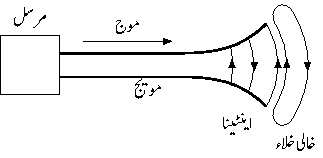
\includegraphics{emtAntennasAndRadiationAntennaDefined}
\caption{اینٹینا وہ عبوری خطہ ہے جہاں منضبط موج ترسیلی نظام سے نکل کر خلاء میں بطور آزاد موج خارج ہوتی ہے۔}
\label{شکل_اینٹینا_تعارف}
\end{figure}

\begin{figure}
\centering
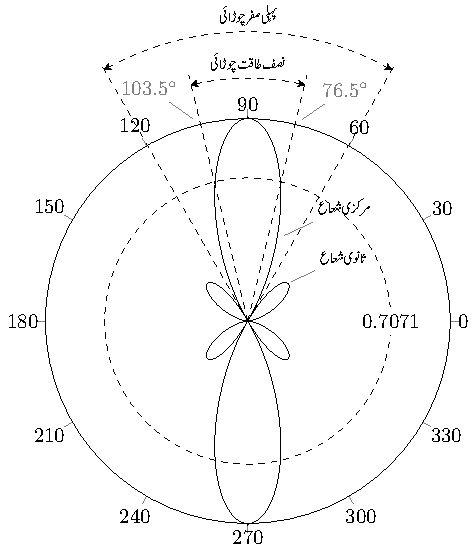
\includegraphics{emtAntennasAndRadiationAntennaLobes}
\caption{اینٹینا کے شعاع کا نقش}
\label{شکل_اینٹینا_شعاع_نقش}
\end{figure}

\حصہ{تاخیری دباو}
کسی بھی اخراجِ شعاع کے نظام میں موج کے ترسیل کے لئے درکار دورانیہ اہمیت رکھتا ہے۔یوں شکل \حوالہ{شکل_اینٹینا_تاخیری_رو} میں دکھائے تار میں برقی رو سے پیدا میدان کا اثر نقطہ \عددیء{N} پر کچھ وقفے سے ہو گا۔خالی خلاء میں یہ وقفہ موج کو تار سے نقطے تک پہنچنے کا دورانیہ \عددیء{\frac{r}{c}} ہے جہاں
 \عددیء{c=\SI{3e8}{\meter/\second}} خالی خلاء میں  شعاع کی رفتار ہے۔یوں \عددیء{N} کے نقطہ نظر سے تار میں برقی رو
\begin{align}
I=I_0 \cos \omega t
\end{align} 
کی بجائے
\begin{align}\label{مساوات_اینٹینا_تاخیری_رو}
[I]=I_0 \cos \omega  \left (t-\frac{r}{c} \right)
\end{align} 
لکھی جا سکتی ہے جہاں \عددیء{[I]} \اصطلاح{تاخیری برقی رو}\فرہنگ{تاخیری!برقی رو}\حاشیہب{retarded current}\فرہنگ{retarded!current} کہلاتی ہے۔تاخیری تفاعل کو چکور قوسین میں بند لکھا جاتا ہے۔تاخیری برقی رو لکھتے ہوئے وقت \عددیء{t} کی جگہ تاخیری وقت \عددیء{(t-\tfrac{r}{c})} استعمال کیا جاتا ہے۔

\begin{figure}
\centering
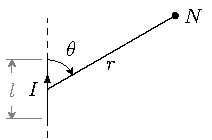
\includegraphics{figAntennaRetardedCurrent}
\caption{برقی رو گزارتی تار کی چھوٹی لمبائی}
\label{شکل_اینٹینا_تاخیری_رو}
\end{figure}

مساوات \حوالہ{مساوات_اینٹینا_تاخیری_رو} کہتا ہے کہ نقطہ \عددیء{N} پر لمحہ \عددیء{t}  پر پیدا اثر،  گزرے  لمحے \عددیء{(t-\tfrac{r}{c})} پر تار میں برقی رو کا اثر ہے جہاں تار سے \عددیء{N} تک فاصلہ \عددیء{r} ہے۔تار سے \عددیء{N} تک شعاع پہنچنے کا دورانیہ \عددیء{\tfrac{r}{c}} ہے۔

گزشتہ بابوں میں امواج کی بات کرتے ہوئے \عددیء{\cos (\omega t -\beta x)} استعمال کیا گیا جس میں \عددیء{\tfrac{\omega}{\beta}=c} کے استعمال سے
\begin{align}
\cos (\omega t -\beta x)=\cos \omega\left( t- \frac{x}{c}\right)
\end{align}
لکھا جا سکتا ہے  جو تاخیری تفاعل کو ظاہر کرتی ہے۔

مساوات \حوالہ{مساوات_اینٹینا_تاخیری_رو} کی دوری سمتیہ شکل
\begin{align}
[I]=I_0 e^{j \omega (t-r/c)}=I_0 e^{j(\omega t-\beta r)}
\end{align}
ہے۔اسی طرح کثافت برقی رو کی تاخیری دوری سمتیہ شکل
\begin{align}
[\kvec{J}]=\kvec{J}_0 e^{j \omega (t-r/c)}=\kvec{J}_0 e^{j(\omega  t -\beta r)}
\end{align}
ہو گی جسے استعمال کرتے ہوئے تاخیری مقناطیسی دباو
\begin{align}\label{مساوات_اینٹینا_تاخیری_سمتی_دباو}
[\kvec{A}]=\frac{\mu}{4\pi}\int_h \frac{[\kvec{J}]}{r}\dif h=\frac{\mu}{4\pi}\int_h \frac{\kvec{J}_0 e^{j\omega(t-r/c)}}{r} \dif h
\end{align}
لکھا جائے گا۔اسی طرح تاخیری حجمی کثافت بار
\begin{align}
[\rho_h]= \rho_0 e^{j\omega \left(t-r/c \right)}
\end{align}
لکھتے ہوئے تاخیری برقی دباو
\begin{align}\label{مساوات_اینٹینا_تاخیری_مقداری_دباو}
[V]=\frac{1}{4\pi \epsilon}\int_h \frac{[\rho_h]}{ r} \dif h
\end{align}
لکھا جائے گا۔ باب-\حوالہ{باب_میکس_ویل} کے آخر میں مساوات \حوالہ{مساوات_میکس_ویل_تاخیری_سمتی_دباو} اور مساوات \حوالہ{مساوات_میکس_ویل_تاخیری_غیر_سمتی_دباو} کے بائیں ہاتھ کے تفاعل کو چکور قوسین میں لکھ کر موج کی رفتار \عددیء{c} لیتے ہوئے اور فاصلے  کو کروی محدد کے رداس \عددیء{r} سے ظاہر کرنے سے  یہی مساوات حاصل ہوتے ہیں۔

ہم یہاں اصل موضوع سے ہٹ کر ایک تکمل پر غور کرتے ہیں جو اس باب میں بار بار استعمال کیا جائے گا۔
%====================
\حصہ{تکمل}\شناخت{حصہ_اینٹینا_تکمل}
شکل \حوالہ{شکل_اینٹینا_تفاعل_کا_تکمل} میں تفاعل \عددیء{f(x)} دکھایا گیا ہے جس کا \عددیء{x_1} تا \عددیء{x_2} تکمل خط کے نیچے دو عمودی نقطہ دار لکیروں کے مابین رقبے کے برابر ہے۔اس رقبے کو \عددیء{K} کہتے ہوئے
\begin{align}
\int_{x_1}^{x_2} f(x) \dif x =K
\end{align}
لکھا جا سکتا ہے۔شکل میں ہلکی سیاہی میں \عددیء{\tfrac{f(x)}{2}} بھی دکھایا گیا ہے جسے \عددیء{\epsilon f(x)} لکھا گیا ہے جہاں \عددیء{\epsilon=0.5} ہے۔چونکہ  \عددیء{x_1} تا \عددیء{x_2} کے ہر نقطے پر تفاعل کی قیمت آدھی ہے لہٰذا ہلکی سیاہی کے خط کے نیچے رقبہ \عددیء{\tfrac{K}{2}} ہو گا لہٰذا
\begin{align}
\int_{x_1}^{x_2} \epsilon f(x) \dif x =\frac{K}{2}=\epsilon K
\end{align}
لکھا جائے گا۔اب فرض کریں کہ \عددیء{\epsilon(x)} مستقل نہیں ہے بلکہ اس کی قیمت \عددیء{x} پر منحصر ہے۔مزید یہ کہ \عددیء{\epsilon(x)} کی قیمت \عددیء{0} تا \عددیء{\epsilon} ممکن ہے۔ایسی صورت میں \عددیء{x_1} تا \عددیء{x_2} پر \عددیء{\epsilon(x) f(x)} کی قیمت \عددیء{0} تا \عددیء{\epsilon f(x)} ممکن ہے لہٰذا \عددیء{\epsilon(x) f(x)} کا تکمل  \عددیء{\epsilon K} سے  کم ہو گا یعنی
\begin{align}
\int_{x_1}^{x_2} \epsilon(x) f(x) \dif x  \le \epsilon  K
\end{align}
جہاں ہر جگہ \عددیء{\epsilon(x)=1} کو بھی مد نظر رکھا گیا ہے۔ اگر \عددیء{\epsilon \to 0} ہو تب تکمل قابل نظر انداز
\begin{align}\label{مساوات_اینٹینا_تکمل_صفر}
\int_{x_1}^{x_2} \epsilon(x) f(x) \dif x  \to 0 \quad \quad (\epsilon \to 0)
\end{align}
 ہو گا۔
\begin{figure}
\centering
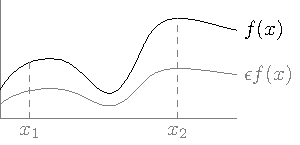
\includegraphics{emtAntennasAndRadiationIntegral}
\caption{تفاعل کا تکمل}
\label{شکل_اینٹینا_تفاعل_کا_تکمل}
\end{figure}

آئیں اب \عددیء{\tfrac{f(x)}{1+\epsilon}} کے تکمل
\begin{align}
\int_{x_1}^{x_2} \frac{f(x)}{1+\epsilon} \dif x
\end{align}
 پر غور کریں جہاں \عددیء{\epsilon \to 0} کے برابر ہے۔ہم
\begin{align}
\frac{1}{1+\epsilon}=(1+\epsilon)^{-1}=1-\frac{\epsilon}{1!}+\frac{\epsilon^2}{2!}-\frac{\epsilon^3}{3!}+\cdots
\end{align}
لکھ سکتے ہیں لہٰذا تکمل
\begin{align}
\int_{x_1}^{x_2} \big(1-\frac{\epsilon}{1!}+\frac{\epsilon^2}{2!}-\frac{\epsilon^3}{3!}+\cdots \big) f(x) \dif x
\end{align}
صورت اختیار کر لے گا۔مساوات \حوالہ{مساوات_اینٹینا_تکمل_صفر} کو استعمال کرتے ہوئے \عددیء{\epsilon \to 0} کی صورت میں اسے
\begin{align}\label{مساوات_اینٹینا_تکمل_رقبہ}
\int_{x_1}^{x_2} \frac{f(x)}{1+\epsilon} \dif x=\int_{x_1}^{x_2} \big(1-\frac{\epsilon}{1!}+\frac{\epsilon^2}{2!}-\frac{\epsilon^3}{3!}+\cdots \big) f(x) \dif x \approx \int_{x_1}^{x_2} f(x) \dif x
\end{align}
لکھا جا سکتا ہے جو \عددیء{K} کے برابر ہے۔

%====================

\حصہ{مختصر جفت قطبی اینٹینا}
مختصر لمبائی کے سیدھے موصل تار کو عموماً مختصر \اصطلاح{ جفت قطب}\فرہنگ{جفت قطب!مختصر}\حاشیہب{short dipole}\فرہنگ{dipole!short} کہا جاتا ہے۔مندرجہ ذیل گفتگو میں مختصر جفت قطب کی لمبائی محدود ہو گی۔لامحدود حد تک کم لمبائی کی صورت میں اسے صغاری جفت قطب\فرہنگ{صغاری جفت قطب}\حاشیہب{infinitesimal} کہا جائے گا۔

خطی نوعیت کے کسی بھی اینٹینا کو متعدد تعداد کے سلسلہ وار جڑے مختصر جفت قطبوں کا مجموعہ تصور کیا جا سکتا ہے لہٰذا مختصر جفت قطب کی خاصیت جانتے ہوئے زیادہ لمبے جفت قطب یا مختلف انداز میں جڑے موصل  تاروں کی خاصیت جاننے میں مدد ملے گی۔ 

\begin{figure}
\centering
\begin{subfigure}{0.4\textwidth}
\centering
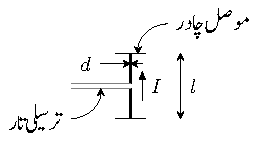
\includegraphics{figAntennaShortDipole}
\caption*{الف: متوازن ترسیلی تار سے جفت قطب کو طاقت مہیا کی گئی ہے۔}
\end{subfigure}%
%
\begin{subfigure}{0.4\textwidth}
\centering
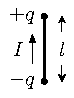
\includegraphics{figAntennaShortDipoleAsShortWire}
\caption*{ب: جفت قطب بطور چھوٹی تار}
\end{subfigure}%
\caption{جفت قطب}
\label{شکل_اینٹینا_جفت_قطب}
\end{figure}



آئیں شکل \حوالہ{شکل_اینٹینا_جفت_قطب}-الف میں دکھائے مختصر جفت قطب پر غور کریں جس کی لمبائی \عددیء{l} طول موج سے بہت کم \عددیء{l\ll \lambda} ہے۔جفت قطب کے سروں پر موصل چادر بطور  کپیسٹر  بوجھ کردار ادا کرتے ہیں۔جفت قطب کی مختصر لمبائی اور اس کے سروں پر موصل چادر مل کر جفت قطب  کی پوری لمبائی پر تقریباً برابر برقی رو رکھنے میں مدد دیتے ہیں۔جیسے شکل-الف میں دکھایا گیا ہے، جفت قطب کو متوازن ترسیلی تار سے طاقت مہیا کی جا سکتی ہے۔یہ فرض کرتے ہوئے کہ ترسیلی تار سے شعاعی اخراج نہیں ہوتی، اس کے موجودگی کو نظر انداز کیا جائے گا۔جفت قطب کے سروں پر نسب موصل چادروں کے شعاعی اخراج کو بھی نظر انداز کیا جائے گا۔جفت قطب کی موٹائی \عددیء{d} اس کے لمبائی سے بہت کم \عددیء{d\ll \lambda} ہے۔ان حقائق کو مد نظر رکھتے ہوئے تحلیلی تجزیے کی خاطر جفت قطب کو شکل \حوالہ{شکل_اینٹینا_جفت_قطب}-ب کی طرح تصور کیا جا سکتا ہے۔ایسا جفت قطب یکساں برقی رو \عددیء{I} گزارتا، \عددیء{l} لمبائی کا تار معلوم ہو گا جس کے دونوں سروں پر برابر مگر الٹ قطب کے بار \عددیء{\mp q} ہوں۔کپیسٹر پر بار \عددیء{q} اور برقی رو \عددیء{I} کا تعلق
\begin{align}\label{مساوات_اینٹینا_رو_اور_بار}
I=\frac{\partial q}{\partial t}
\end{align}
ہے۔ 

\begin{figure}
\centering
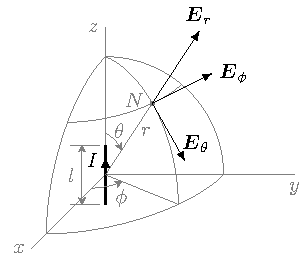
\includegraphics{figAntennaDipoleAtOriginWithFarField}
\caption{جفت قطب محدد کے مرکز پر ہے۔مرکز سے دور نقطہ \عددی{N} پر دور میدان کے اجزاء بھی دکھائے گئے ہیں۔}
\label{شکل_اینٹینا_جفت_قطب_اور_اس_کے_دور_میدان}
\end{figure}

آئیں لامحدود وسعت کی خالی خلاء میں جفت قطب کے میدان حاصل کریں۔جیسے شکل \حوالہ{شکل_اینٹینا_جفت_قطب_اور_اس_کے_دور_میدان} میں دکھایا گیا ہے، جفت قطب کے وسط کو کروی محدد کے مرکز اور لمبائی کو \عددیء{z} محدد پر رکھتے ہوئے آگے بڑھتے ہیں۔کسی بھی نقطہ \عددیء{N} پر عموماً آپس میں عمودی تین میدان \عددیء{E_r}، \عددیء{E_{\theta}} اور \عددیء{E{\phi}} پائے جائیں گے۔


کسی بھی نقطہ \عددیء{N} پر مساوات \حوالہ{مساوات_میکس_ویل_تاخیری_مقناطیسی_میدان}  اور مساوات \حوالہ{مساوات_میکس_ویل_تاخیری_برقی_میدان} بالترتیب مقناطیسی میدان اور برقی میدان دیتے ہیں
\begin{align}
\kvec{H}=\frac{1}{\mu_0}\nabla \times \kvec{A} \\
\kvec{E}=-\nabla V-\frac{\partial \kvec{A}}{\partial t}
\end{align}
جہاں
\begin{description}
\جزو{$V$} نقطہ \عددیء{N} پر مقداری برقی دباو
\جزو{$\kvec{A}$} نقطہ \عددیء{N} پر سمتی دباو
\end{description}
ہیں۔اگر ہمیں کسی بھی نقطے پر مقداری دباو \عددیء{V} اور سمتی دباو \عددیء{\kvec{A}} معلوم ہوں تب مندرجہ بالا دو مساوات سے اس نقطے پر برقی اور مقناطیسی میدان حاصل کئے جا سکتے ہیں۔چونکہ ہمیں  جفت قطب سے دور میدان درکار ہیں لہٰذا ایسی صورت میں مساوات \حوالہ{مساوات_اینٹینا_تاخیری_سمتی_دباو} اور مساوات \حوالہ{مساوات_اینٹینا_تاخیری_مقداری_دباو} میں دئے تاخیری دباو قابل استعمال ہوں گے۔یوں ان مساوات کو
\begin{align}
\kvec{H}&=\frac{1}{\mu_0}\nabla \times [\kvec{A}] \label{مساوات_اینٹینا_عمومی_مقناطیسی}\\
\kvec{E}&=-\nabla [V]-\frac{\partial [\kvec{A}]}{\partial t}=-\nabla [V]-j \omega [\kvec{A}]\label{مساوات_اینٹینا_عمومی_برقی}
\end{align}
لکھا جا سکتا ہے جہاں مساوات \حوالہ{مساوات_میکس_ویل_بدلتا_میدان_غیر_سمتی_دباو} اور مساوات \حوالہ{مساوات_میکس_ویل_بدلتا_میدان_سمتی_دباو} سے تاخیری دباو
\begin{align}
[\kvec{A}]&=\frac{\mu_0}{4\pi} \int_h \frac{\kvec{J}_0 e^{j \omega(t-r/c)}}{r} \dif h \label{مساوات_اینٹینا_عمومی_سمتی_دباو}\\
[V]&=\frac{1}{4\pi\epsilon_0}\int_h \frac{\rho_0 e^{j\omega(t-r/c)}}{r} \dif h\label{مساوات_اینٹینا_عمومی_مقداری_دباو}
\end{align}
لکھے جا سکتے ہیں۔

کسی بھی برقی بار اور برقی رو سے پیدا میدان مساوات \حوالہ{مساوات_اینٹینا_عمومی_مقناطیسی} اور مساوات \حوالہ{مساوات_اینٹینا_عمومی_برقی} سے حاصل کئے جا سکتے ہیں۔مساوات \حوالہ{مساوات_اینٹینا_عمومی_مقداری_دباو} کے تحت تاخیری مقداری دباو \عددیء{[V]} صرف ساکن باروں پر منحصر ہے جبکہ مساوات \حوالہ{مساوات_اینٹینا_عمومی_سمتی_دباو} کے تحت  تاخیری سمتی دباو \عددیء{[\kvec{A}]} صرف برقی رو یعنی حرکت کرتے باروں پر منحصر ہے۔مساوات \حوالہ{مساوات_اینٹینا_عمومی_مقناطیسی} کے تحت مقناطیسی میدان \عددیء{\kvec{H}} صرف برقی رو یعنی حرکت کرتے باروں پر منحصر ہے جبکہ مساوات \حوالہ{مساوات_اینٹینا_عمومی_برقی} کے تحت برقی میدان \عددیء{\kvec{E}} ساکن بار اور برقی رو دونوں پر منحصر ہے۔ہم جلد مساوات \حوالہ{مساوات_اینٹینا_دور_میدان_برقی_رو_سے_حصول} میں دیکھیں گے کہ کسی بھی بار اور برقی رو سے  دور پیدا مقناطیسی اور برقی میدانوں کا دارومدار صرف برقی رو پر ہوتا ہے۔ چونکہ اس باب میں تاخیری دباو ہی استعمال کئے جائیں گے لہٰذا انہیں چکور قوسین میں لکھنے سے گریز کیا جائے گا۔اس باب میں یہاں سے آگے بغیر چکور قوسین کے دباو کو تاخیری دباو ہی سمجھا جائے۔

\begin{figure}
\centering
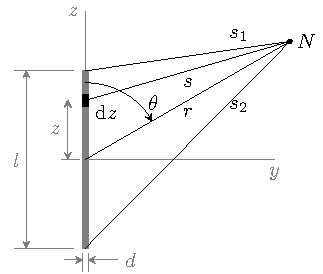
\includegraphics{figAntennaDipoleGeometry}
\caption{جفت قطب اور دور میدان۔}
\label{شکل_اینٹینا_جفت_قطب_اور_دور_میدان}
\end{figure}
شکل \حوالہ{شکل_اینٹینا_جفت_قطب_اور_اس_کے_دور_میدان} یا شکل \حوالہ{شکل_اینٹینا_جفت_قطب_اور_دور_میدان} سے ظاہر ہے کہ سمتی دباو کا صرف \عددیء{\az} جزو
\begin{align}\label{مساوات_اینٹینا_جفت_قطب_سمتی_دباو_حصول}
\kvec{A}=\frac{\az \mu_0 }{4\pi} \int_{-l/2}^{l/2} \frac{I_0 e^{j(\omega t -\beta s)}}{s} \dif z
\end{align}
 پایا جاتا ہے۔اگر جفت قطب کی لمبائی \عددیء{l}، نقطہ \عددیء{N} سے جفت قطب تک فاصلہ \عددیء{r} سے نہایت کم \عددیء{l\ll r} اور طول موج \عددیء{\lambda} سے بھی نہایت کم \عددیء{l \ll \lambda} ہو تب مندرجہ بالا مساوات میں متغیر فاصلہ \عددیء{s} کی جگہ مستقل فاصلہ \عددیء{r} پر کیا جا سکتا ہے\حاشیہد{جیسے حصہ \حوالہ{حصہ_اینٹینا_تکمل} میں دکھایا گیا ہے۔} اور ساتھ ہی ساتھ \عددیء{l} پر مختلف نقطوں سے  \عددیء{N} پر پیدا دباو میں زاویائی فرق کو نظر انداز کیا جا سکتا ہے۔اس طرح ان تمام کو تکمل کے باہر لے جایا جا سکتا ہے۔جفت قطب کی پوری لمبائی پر یک برابر برقی رو \عددیء{I_0} کی صورت میں \عددیء{I_0} کو بھی تکمل کے باہر لے جایا جا سکتا ہے۔یوں مندرجہ بالا مساوات سے
\begin{align}\label{مساوات_اینٹینا_جفت_قطب_سمتی_دباو_حاصل}
\kvec{A} =\frac{\az \mu_0 I_0 l e^{j(\omega t -\beta r)}}{4\pi r}
\end{align}
حاصل ہوتا ہے۔ اس مساوات کو کروی محدد میں یوں
\begin{align*}
\kvec{A}=A_r \ar +A_{\theta} \atheta +A_{\phi} \aphi
\end{align*}
لکھا جائے گا جہاں
\begin{gather}
\begin{aligned}\label{مساوات_اینٹینا_کروی_سمتی_دباو}
A_r&=\ar \cdot \kvec{A}= \frac{ \mu_0 I_0 l e^{j(\omega t -\beta r)}}{4\pi r} \ar \cdot \az= \frac{ \mu_0 I_0 l e^{j(\omega t -\beta r)}}{4\pi r} \cos \theta\\
A_{\theta}&=\atheta \cdot \kvec{A}=\frac{ \mu_0 I_0 l e^{j(\omega t -\beta r)}}{4\pi r} \atheta \cdot \az =-\frac{ \mu_0 I_0 l e^{j(\omega t -\beta r)}}{4\pi r} \sin \theta \\
A_{\phi}&=\aphi \cdot \kvec{A}=\frac{ \mu_0 I_0 l e^{j(\omega t -\beta r)}}{4\pi r} \aphi \cdot \az =0
\end{aligned}
\end{gather}
ہوں گے جہاں اکائی سمتیات کے مقداری ضرب صفحہ \حوالہصفحہ{جدول_سمتیہ_کروی_نلکی_اکائی_غیر-سمتی_ضرب} پر جدول \حوالہ{جدول_سمتیہ_کروی_نلکی_اکائی_غیر-سمتی_ضرب} سے حاصل کئے گئے۔اس طرح 
\begin{align}\label{مساوات_اینٹینا_جفت_قطب_سمتی_دباو}
\kvec{A}=\frac{ \mu_0 I_0 l e^{j(\omega t -\beta r)}}{4\pi r}\left(\cos \theta \ar-\sin \theta \atheta \right)
\end{align}
لکھا جائے گا۔

ساکن بار جفت قطب کے سروں پر پایا جاتا ہے لہٰذا مقداری دباو
\begin{align}\label{مساوات_اینٹینا_مقداری_دباو_الف}
V=\frac{q_0}{4\pi \epsilon_0} \left[\frac{e^{j(\omega t -\beta s_1)}}{s_1} -\frac{e^{j(\omega t -\beta s_2)}}{s_2}\right]
\end{align}
ہو گا جہاں مساوات \حوالہ{مساوات_اینٹینا_رو_اور_بار} کے تحت
\begin{align}\label{مساوات_اینٹینا_رو_اور_بار_ب}
q=\int I \dif t=\frac{I}{j\omega }
\end{align}
کے برابر ہے جہاں
\begin{align*}
I&=I_0 e^{j(\omega t -\beta s)}\\
q&=q_0  e^{j(\omega t -\beta s)}
\end{align*}
ہیں۔مساوات \حوالہ{مساوات_اینٹینا_رو_اور_بار_ب} سے \عددیء{q_0=\tfrac{I_0}{j\omega}} حاصل کرتے ہوئے مساوات \حوالہ{مساوات_اینٹینا_مقداری_دباو_الف} میں پر کرتے ہیں۔ 
\begin{align}\label{مساوات_اینٹینا_مقداری_دباو_ب}
V=\frac{I_0}{4\pi \epsilon_0 j \omega } \left[\frac{e^{j(\omega t -\beta s_1)}}{s_1} -\frac{e^{j(\omega t -\beta s_2)}}{s_2}\right]
\end{align}
%
\begin{figure}
\centering
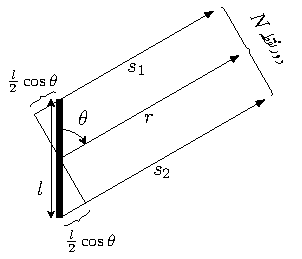
\includegraphics{figAntennaDipoleGeometryFarAway}
\caption{جفت قطب اور دور نقطے کے تعلق۔}
\label{شکل_اینٹینا_جفت_قطب_تعلق}
\end{figure}
شکل \حوالہ{شکل_اینٹینا_جفت_قطب_تعلق} کو دیکھ کر
\begin{align*}
s_1&=r-\frac{l}{2}\cos \theta\\
s_2&=r+\frac{l}{2}\cos \theta
\end{align*}
لکھے جا سکتے ہیں جنہیں مساوات \حوالہ{مساوات_اینٹینا_مقداری_دباو_ب} میں پر کرتے
\begin{align}
V=\frac{I_0 e^{j(\omega t -\beta r)}}{4\pi \epsilon_0 j \omega}\left[\frac{(r+\frac{l}{2}\cos \theta) e^{j\frac{\beta l}{2}\cos \theta}-(r-\frac{l}{2}\cos \theta) e^{-j\frac{\beta l}{2}\cos \theta}}{r^2-\frac{l^2}{4}\cos^2 \theta} \right]
\end{align}
ملتا ہے۔چکور قوسین میں شرح کے نچلے حصے میں \عددیء{r \gg l} کی وجہ سے  \عددیء{\tfrac{l^2}{4}\cos^2 \theta} کو نظر انداز کرتے ہیں۔\اصطلاح{مسئلہ ڈی موے ور}\فرہنگ{مسئلہ!ڈی موے ور}\فرہنگ{ڈی موے ور!مسئلہ}\حاشیہب{$(e^{j\alpha}=\cos \alpha + j \sin \alpha)$ de Moivre's theorem}\فرہنگ{de Moivre} کے استعمال سے
\begin{multline}\label{مساوات_اینٹینا_مقداری_دباو_پ}
V=\frac{I_0 e^{j(\omega t -\beta r)}}{4\pi \epsilon_0 j \omega r^2} \left[\left(r+\frac{l}{2}\cos \theta\right) \left(\cos \frac{\beta l \cos \theta}{2} +j \sin \frac{\beta l \cos \theta}{2}\right)\right.\\
-\left.\left(r-\frac{l}{2}\cos \theta\right) \left(\cos \frac{\beta l \cos \theta}{2} -j \sin \frac{\beta l \cos \theta}{2}\right) \right]
\end{multline}  
لکھا جائے گا۔چونکہ \عددیء{l \ll \lambda} ہے لہٰذا 
\begin{align*}
\cos \frac{\beta l \cos \theta}{2}&=\cos \frac{\pi l \cos \theta}{\lambda}\approx l\\
\sin \frac{\beta l \cos \theta}{2}&\approx \frac{\beta l \cos \theta}{2}
\end{align*}
ہوں گے، جنہیں مساوات \حوالہ{مساوات_اینٹینا_مقداری_دباو_پ} میں پر کرنے سے
\begin{align}\label{مساوات_اینٹینا_مقداری_دباو_ت}
V=\frac{I_0 l e^{j(\omega t -\beta r)} \cos \theta}{4\pi \epsilon_0 c}\left(\frac{1}{r}+\frac{c}{j\omega r^2} \right)
\end{align}
حاصل ہوتا ہے جہاں
\begin{description}
\جزو{$I_0$} برقی رو کا حیطہ یعنی اس کی زیادہ سے زیادہ قیمت، \عددیء{\si{\ampere}}
\جزو{$l$} جفت قطب کی لمبائی، \عددیء{\si{\meter}}
\جزو{$\omega$}  زاویائی تعدد \عددیء{(\omega=2\pi f)} ، اکائی \عددیء{\si{\radian / \second}}۔ جہاں ہرٹز \عددیء{\si{\hertz}}میں تعدد \عددیء{f} ہے
\جزو{$\beta$} زاویائی مستقل \عددیء{(\beta=\tfrac{2\pi}{\lambda})}، اکائی \عددیء{\si{\radian /\meter}}
\جزو{$t$}وقت،\عددیء{\si{\second}} 
\جزو{$\theta$}جفت قطب اور جفت قطب سے نقطہ \عددیء{N} تک سمتیہ کے مابین زاویہ
\جزو{$\epsilon_0$}خالی خلاء کا برقی مستقل، \عددیء{\SI{8.854}{\pico\farad/\meter}}
\جزو{$c$}خالی خلاء میں شعاع کی رفتار، \عددیء{\SI{3e8}{\meter/\second}}
\جزو{$j$}خیالی عدد \عددیء{\sqrt{-1}}
\جزو{$r$}جفت قطب کے وسط سے نقطہ \عددیء{N} تک فاصلہ،\عددیء{\si{\meter}}
\end{description}
ہیں۔

مختصر جفت قطب کے وسط سے، \عددیء{l \ll \lambda} اور \عددیء{l \ll r} کی صورت میں، \عددیء{r} فاصلے اور \عددیء{\theta} زاویے پر مساوات \حوالہ{مساوات_اینٹینا_جفت_قطب_سمتی_دباو} سمتی دباو اور مساوات \حوالہ{مساوات_اینٹینا_مقداری_دباو_ت} مقداری دباو دیتے ہیں۔کروی محدد میں مقداری دباو کی ڈھلوان
\begin{gather}
\begin{aligned}
\nabla V&=\frac{\partial V}{\partial r}\ar+\frac{1}{r}\frac{\partial V}{\partial \theta}\atheta+\frac{1}{r\sin \theta} \frac{\partial V}{\partial \phi}\aphi\\
&=\frac{I_0 l e^{j(\omega t -\beta r)}}{4\pi \epsilon_0 c}\left[-\left(\frac{ \cos \theta}{r^2}+\frac{2 c  \cos \theta}{j\omega r^3} \right)\ar -\left(\frac{\sin \theta}{r^2}+\frac{c \sin \theta}{j\omega r^3} \right) \atheta\right]
\end{aligned}
\end{gather}
کے برابر ہے۔برقی میدان \عددیء{\kvec{E}=E_r \ar +E_{\theta} \atheta+E_{\phi}\aphi} کے اجزاء مساوات \حوالہ{مساوات_اینٹینا_عمومی_برقی} کی مدد سے 
\begin{align*}
E_r&=-j \omega A_r-\frac{\partial V}{\partial r}\\
E_{\theta}&=-j \omega A_{\theta}-\frac{1}{r}\frac{\partial V}{\partial \theta}\\
E_{\phi}&=-j \omega A_{\phi}-\frac{1}{r\sin \theta}\frac{\partial V}{\partial \phi}
\end{align*}
لکھے جا سکتے ہیں جن میں مطلوبہ تفاعل پر کرنے سے برقی میدان کے عمومی مساوات
\begin{gather}
\begin{aligned}\label{مساوات_اینٹینا_جفت_قطب_برقی_اجزاء}
E_r&=\frac{I_0 l \cos \theta e^{j(\omega t -\beta r)}}{2\pi \epsilon_0}\left(\frac{1}{c r^2}+\frac{1}{j \omega r^3} \right)\\
E_{\theta}&=\frac{I_0 l \sin \theta e^{j(\omega t -\beta r)}}{4\pi \epsilon_0}\left(\frac{j \omega}{c^2 r}+\frac{1}{c r^2}+\frac{1}{j \omega r^3} \right)\quad \quad \text{\RL{عمومی میدان}}\\
E_{\phi}&=0 
\end{aligned}
\end{gather}
حاصل ہوتے ہیں۔

مقناطیسی میدان مساوات \حوالہ{مساوات_اینٹینا_عمومی_مقناطیسی} سے حاصل ہو گی۔کروی محدد میں سمتی دباو کی گردش
\begin{multline}
\kvec{B}=\nabla \times \kvec{A}=\frac{1}{r \sin \theta}\left[\frac{\partial (A_{\theta}  \sin \theta)}{\partial \theta}-\frac{\partial A_{\theta} }{\partial \phi} \right]\ar+\frac{1}{r }\left[\frac{1}{\sin \theta}\frac{\partial A_r }{\partial \phi}-\frac{\partial (r A_{\phi} )}{\partial r} \right]\atheta
\\
 +\frac{1}{r}\left[\frac{\partial (r A_\theta )}{\partial r}-\frac{\partial A_r }{\partial \theta} \right]\aphi
\end{multline}
میں مساوات \حوالہ{مساوات_اینٹینا_کروی_سمتی_دباو} پر کرنے سے مقناطیسی میدان کی عمومی مساوات
\begin{gather}
\begin{aligned}\label{مساوات_اینٹینا_جفت_قطب_مقناطیسی_اجزاء}
H_{\phi}&=\frac{I_0 l \sin \theta e^{j(\omega t -\beta r)}}{4\pi} \left(\frac{j \omega}{c r}+\frac{1}{r^2} \right)\quad \quad\text{\RL{عمومی میدان}}\\
H_r&=0\\
H_{\theta}&=0 
\end{aligned}
\end{gather}
حاصل ہوتے ہیں جہاں \عددیء{\kvec{B}=\mu_0 \kvec{H}} کا استعمال کیا گیا۔

مساوات \حوالہ{مساوات_اینٹینا_جفت_قطب_برقی_اجزاء} اور مساوات \حوالہ{مساوات_اینٹینا_جفت_قطب_مقناطیسی_اجزاء} کے تحت جفت قطب سے پیدا  میدان کے صرف تین اجزاء \عددیء{E_r}، \عددیء{E_{\theta}} اور \عددیء{H_{\phi}} پائے جاتے ہیں۔جفت قطب سے زیادہ فاصلے پر میدان کی مساوات میں ایسے اجزاء جن میں \عددیء{\tfrac{1}{r^2}} یا \عددیء{\tfrac{1}{r^3}} پایا جاتا ہو کو نظر انداز کیا جا سکتا ہے۔یوں \عددیء{E_r} قابل نظر انداز ہو گا لہٰذا \عددیء{E_r \approx 0} تصور کیا جائے گا جبکہ
\begin{gather}
\begin{aligned}\label{مساوات_اینٹینا_جفت_قطب_دور_میدان}
E_{\theta}&=\frac{I_0 l \sin \theta e^{j(\omega t -\beta r)}}{4\pi \epsilon_0 }\frac{j \omega}{c^2 r}=j \frac{30 I_0 \beta l}{r} \sin \theta e^{j(\omega t-\beta r)}\\
H_{\phi}&=\frac{ I_0 l \sin \theta e^{j(\omega t -\beta r)}}{4\pi }\frac{j \omega}{c r}=j\frac{I_0 \beta l}{4\pi r} \sin \theta e^{j(\omega t -\beta r)}\quad \quad \text{\RL{دور میدان}}
\end{aligned}
\end{gather} 
ہوں گے۔مساوات \حوالہ{مساوات_اینٹینا_جفت_قطب_دور_میدان} استعمال کرتے ہوئے برقی اور مقناطیسی میدان کی شرح
\begin{align}
\frac{E_{\theta}}{H_{\phi}}=\frac{1}{\epsilon_0 c}=\sqrt{\frac{\mu_0}{\epsilon_0}}=\SI{376.7}{\ohm}
\end{align}
حاصل ہوتی ہے جو خالی خلاء کی قدرتی رکاوٹ \عددی{Z_0} ہے۔

یہاں اس حقیقت پر توجہ دیں کہ خالی خلاء میں \عددیء{\TEM} موج کی طرح، جفت قطب سے دور \عددیء{E_{\theta}} اور \عددیء{H_{\phi}}  آپس میں ہم قدم ہیں۔اس کے علاوہ دونوں میدان  \عددیء{\sin \theta} کے راست تناسب ہیں یعنی جفت قطب کے محوری سمت \عددیء{\theta=0^{\circ}} پر ان کی قیمت صفر جبکہ \عددیء{\theta=90^{\circ}} پر ان کی قیمت زیادہ سے زیادہ ہے۔اندرسہ\فرہنگ{اندرسہ}\حاشیہب{doughnut}\فرہنگ{doughnut} شکل کی ان میدان کو شکل \حوالہ{شکل_اینٹینا_اندرسہ_دور_میدان}-الف میں دکھایا گیا ہے جبکہ شکل-ب میں  کارتیسی  محدد کی سطح \عددی{x=0} پر دور میدان کا عمودی تراش دکھایا گیا ہے۔شکل-الف میں اندرسے کے محور پر جفت قطب پایا جاتا ہے جسے شکل-ب میں \عددی{z} محدد پر موٹی لکیر سے ظاہر کیا گیا ہے۔ 

\begin{figure}
\centering
\begin{subfigure}{0.4\textwidth}
\centering
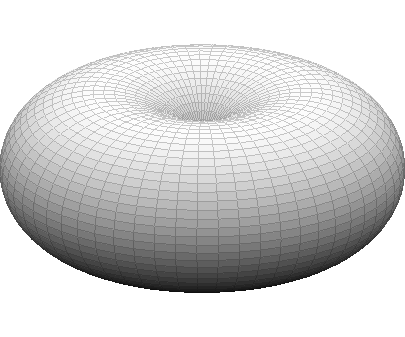
\includegraphics{figAntennaToroidalRadiationPattern}
\caption{}
\end{subfigure}%
%
\begin{subfigure}{0.4\textwidth}
\centering
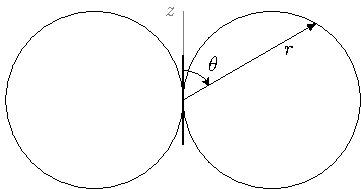
\includegraphics{figAntennaToroidalRadiationPatternCrossSection}
\caption{}
\end{subfigure}%
\caption{اندرسہ شکل کا دور میدان۔}
\label{شکل_اینٹینا_اندرسہ_دور_میدان}
\end{figure}

جفت قطب سے دور میدان حاصل کرتے وقت مساوات \حوالہ{مساوات_اینٹینا_جفت_قطب_برقی_اجزاء} اور مساوات \حوالہ{مساوات_اینٹینا_جفت_قطب_مقناطیسی_اجزاء} میں \عددیء{\tfrac{1}{r^2}} یا \عددیء{\tfrac{1}{r^3}} رکھتے اجزاء کو نظر انداز کیا گیا یعنی \عددیء{E_{\theta}} میں 
\begin{align*}
\abs{j\frac{ \omega}{c^2 r}} & \gg \frac{1}{c r^2}\\
\abs{j\frac{ \omega}{c^2 r}} &\gg \abs{\frac{1}{j \omega r^3}} 
\end{align*}
یا
\begin{align}
r \gg \frac{c}{\omega}
\end{align}
تصور کیا گیا۔اسی طرح \عددیء{H_{\phi}} میں بھی
\begin{align*}
\abs{j \frac{ \omega}{c r}} \gg \frac{1}{r^2}
\end{align*}
یا
\begin{align}
r \gg \frac{c}{\omega}
\end{align}
تصور کیا گیا جسے
\begin{align}
r \gg \frac{1}{\beta} \quad \quad (\text{\RL{دور میدان}})
\end{align}
بھی لکھا جا سکتا ہے۔اگر جفت قطب کے قریب میدان کی بات کی جائے تو \عددیء{r \ll \tfrac{c}{\omega}} یعنی \عددیء{r \ll \tfrac{1}{\beta}} لیا جائے گا۔یوں مساوات \حوالہ{مساوات_اینٹینا_جفت_قطب_برقی_اجزاء} اور مساوات \حوالہ{مساوات_اینٹینا_جفت_قطب_مقناطیسی_اجزاء} میں
\begin{align*}
\frac{1}{c r^2}& \ll \abs{\frac{1}{j \omega r^3}}\\
\abs{\frac{j \omega}{c^2 r}}& \ll \abs{\frac{1}{j \omega r^3}}\\
\frac{1}{c r^2}& \ll \abs{\frac{1}{j \omega r^3}} \\
\abs{\frac{j \omega}{c r}}& \ll \frac{1}{r^2}
\end{align*}
ہوں گے لہٰذا قریبی میدان
\begin{gather}
\begin{aligned}\label{مساوات_اینٹینا_جفت_قطب_قریب_میدان}
E_r&=\frac{I_0 l \cos \theta e^{j(\omega t -\beta r)}}{2\pi \epsilon_0 }\frac{1}{j \omega r^3} =\frac{I_0 l \cos \theta e^{j(\omega t -\beta r-\tfrac{\pi}{2})}}{2\pi \epsilon_0 \omega r^3}\\
E_{\theta}&=\frac{I_0 l \sin \theta e^{j(\omega t -\beta r)}}{4\pi \epsilon_0}\frac{1}{j \omega r^3}=\frac{I_0 l \sin \theta e^{j(\omega t -\beta r-\tfrac{\pi}{2})}}{4\pi \epsilon_0 \omega r^3}\\
H_{\phi}&=\frac{I_0 l \sin \theta e^{j(\omega t -\beta r)}}{4\pi}\frac{1}{r^2}=\frac{I_0 l \sin \theta e^{j(\omega t -\beta r)}}{4\pi r^2} \quad \text{\RL{قریبی میدان}}
\end{aligned}
\end{gather}
لکھے جا سکتے ہیں۔ کل قریبی برقی میدان
\begin{align}\label{مساوات_اینٹینا_قریب_کل_برقی}
\kvec{E}=E_r \ar+E_{\theta}\atheta=\left[\frac{I_0 l \cos \theta }{2\pi \epsilon_0 \omega r^3}\ar+\frac{I_0 l \sin \theta }{4\pi \epsilon_0 \omega r^3}\atheta\right]e^{j(\omega t -\beta r-\tfrac{\pi}{2})}
\end{align}
ہو گا۔مساوات \حوالہ{مساوات_اینٹینا_قریب_کل_برقی} کے برقی میدان میں جزو ضربی \عددیء{e^{j(\omega t -\beta r-\tfrac{\pi}{2})}} پایا جاتا ہے جبکہ مقناطیسی میدان میں جزو ضربی \عددیء{e^{j(\omega t -\beta r)}} پایا جاتا ہے۔یوں جفت قطب کے قریب کسی بھی نقطے پر ہر لمحہ برقی میدان  اور مقناطیسی میدان میں \عددیء{\tfrac{\pi}{2}} زاویے کا فرق پایا جاتا ہے جو ساکن میدان کی نشانی ہے۔

جفت قطب کے قریب برقی اور مقناطیسی میدان میں لمحاتی طور \عددیء{\tfrac{\pi}{2}} ریڈیئن  کا زاویہ پایا جاتا ہے جبکہ جفت قطب سے دور دونوں میدان لمحاتی طور پر ہم قدم ہیں لہٰذا کسی درمیانے فاصلے پر ان میدانوں میں \عددیء{45^{\circ}} کا زاویہ ہو گا۔

یوں جفت قطب کے انتہائی قریب کسی بھی نقطے پر مقناطیسی اور برقی میدان میدان میں \عددی{90^{\circ}} کا زاویائی فرق پایا جاتا ہے۔جفت قطب سے فاصلہ بڑھانے سے زاویائی فرق \عددی{45^{\circ}} ہو جاتا ہے جبکہ جفت قطب سے بہت دور دونوں میدان ہم قدم ہوتے ہیں۔اسے تمام کو یوں بیان کیا جا سکتا ہے کہ فاصلہ بڑھانے سے برقی میدان وقت کی نسبت سے گھوم کر مقناطیسی میدان کے ہم قدم ہو جاتا ہے۔

مخلوط پوئنٹنگ سمتیہ استعمال کرتے ہوئے مساوات \حوالہ{مساوات_اینٹینا_جفت_قطب_دور_میدان} سے  دور میدان میں کثافت توانائی
\begin{align*}
\pmb{\mathscr{P}}_{\text{اوسط}}=\frac{1}{2}\left[\kvec{E} \times \kvec{H}^*\right]_{\text{حقیقی}}=\frac{1}{2}E_{\theta} H_{\phi}^* \ar=\frac{15 I_0^2 \beta^2 l^2}{4 \pi r^2} \sin^2 \theta \ar \quad \text{\RL{دور کثافت طاقت}}
\end{align*}
حاصل ہوتی ہے جو  رداسی \عددیء{r} سمت میں منتقل ہوتی حقیقی توانائی ہے۔یہی اینٹینا کی شعاعی اخراج ہے۔شعاعی اخراج \عددیء{\theta=90^{\circ}} پر زیادہ سے زیادہ ہے۔اسی طرح پوئنٹنگ سمتیہ استعمال کرتے ہوئے مساوات \حوالہ{مساوات_اینٹینا_جفت_قطب_قریب_میدان} سے قریبی میدان میں کثافت توانائی
\begin{align*}
\frac{1}{2}\left[\kvec{E} \times \kvec{H}^*\right]_{\text{حقیقی}}&=\frac{1}{2}\left[(E_{r} \ar+E_{\theta} \atheta) \times H_{\phi}^* \aphi\right]_{\text{حقیقی}}\\
&=\frac{1}{2}\left[-\frac{I_0 l \cos \theta }{2\pi \epsilon_0 \omega r^3}\atheta+\frac{I_0 l \sin \theta }{4\pi \epsilon_0 \omega r^3}\ar \right]\frac{I_0 l \sin \theta }{4\pi r^2} e^{-j\tfrac{\pi}{2}}\\
\end{align*}
حاصل ہوتی ہے جس کا بیشتر حصہ خیالی ہے اور ساتھ ہی ساتھ شعاعی اخراج کے علاوہ یہاں \عددیء{\theta} سمت میں گھومتی طاقت بھی پائی جاتی ہے۔

آئیں اب نہایت کم تعدد پر صورت حال دیکھیں۔ مساوات \حوالہ{مساوات_اینٹینا_جفت_قطب_برقی_اجزاء} میں \عددیء{I_0=j \omega q_0} پر کرتے ہوئے اور مساوات \حوالہ{مساوات_اینٹینا_جفت_قطب_مقناطیسی_اجزاء} کو جوں کا توں دوبارہ پیش کرتے ہیں۔
\begin{align*}
E_r&=\frac{q_0 l \cos \theta e^{j(\omega t -\beta r)}}{2\pi \epsilon_0}\left(\frac{j \omega}{c r^2}+\frac{1}{ r^3} \right)\\
E_{\theta}&=\frac{q_0 l \sin \theta e^{j(\omega t -\beta r)}}{4\pi \epsilon_0}\left(-\frac{\omega^2 }{c^2 r}+\frac{j \omega }{c r^2}+\frac{1}{ r^3} \right)\\
H_{\phi}&=\frac{I_0 l \sin \theta e^{j(\omega t -\beta r)}}{4\pi} \left(\frac{j \omega}{c r}+\frac{1}{r^2} \right)
\end{align*}
\عددیء{\abs{e^{-j\beta r}}=1} لیتے ہوئے، صفر کے قریب تر تعدد \عددیء{\omega \to 0} پر ان مساوات سے میدان کی حتمی قیمت
\begin{align*}
E_r&=\frac{q_0 l \cos \theta}{2\pi \epsilon_0 r^3}\\
E_{\theta}&=\frac{q_0 l \sin \theta }{4\pi \epsilon_0 r^3}\\
H_{\phi}&=\frac{I_0 l \sin \theta }{4\pi r^2} \quad \quad \text{\RL{نیم ساکن میدان}}
\end{align*}
حاصل ہوتی ہیں جن سے برقی میدان
\begin{align}
\kvec{E}=\frac{q_0 l }{4\pi \epsilon_0 r^3}\left(2\cos \theta \ar+\sin \theta \atheta \right)
\end{align}
لکھا جا سکتا ہے۔ان میدان کو \اصطلاح{نیم ساکن میدان}\فرہنگ{میدان!نیم ساکن}\حاشیہب{quasi stationary fields}\فرہنگ{quasi stationary fields} کہا جاتا ہے۔یہ صفحہ \حوالہصفحہ{مساوات_توانائی_جفت_قطب_دور_میدان_الف} پر حاصل کی گئی مساوات \حوالہ{مساوات_توانائی_جفت_قطب_دور_میدان_الف} ہی ہے۔اسی طرح مندرجہ بالا مقناطیسی میدان \عددیء{H_{\phi}} کی قیمت صفحہ \حوالہصفحہ{مساوات_مقناطیسی_تار_کا_ٹکڑا_اور_میدان} پر مساوات \حوالہ{مساوات_مقناطیسی_تار_کا_ٹکڑا_اور_میدان} ہی ہے۔چونکہ یہ میدان \عددیء{\tfrac{1}{r^2}} یا \عددیء{\tfrac{1}{r^3}} کے تعلق سے تبدیل ہوتے ہیں لہٰذا یہ جفت قطب کے قریب ہی پائے جاتے ہیں۔جفت قطب سے دور ان کی قیمت قابل نظر انداز ہوتی ہے لہٰذا ان کا شعاعی اخراج میں خاص کردار نہیں ہوتا۔بلند تعدد پر دور میدان جنہیں مساوات \حوالہ{مساوات_اینٹینا_جفت_قطب_دور_میدان} پیش کرتی ہے، \عددیء{\tfrac{1}{r}} کے تعلق سے گھٹتی ہیں لہٰذا یہی شعاعی اخراج کو ظاہر کرتی ہیں اور یوں انہیں \اصطلاح{اخراجی میدان}\فرہنگ{اخراجی میدان}\حاشیہب{radiation fields}\فرہنگ{radiation fields} کہا جاتا ہے۔

مختصر جفت قطب، \عددیء{l \ll r} اور \عددیء{l \ll \lambda}، کے تمام میدان کو جدول \حوالہ{جدول_اینٹینا_مختصر_جفت_قطب} میں پیش کیا گیا ہے۔بقایا اجزاء \عددیء{E_{\phi}=H_r=H_{\theta}=0} صفر  کے برابر ہیں۔
\begin{table}
\caption{مختصر جفت قطب کے میدان}
\centering
\begin{tabular}{l l l l}
\hline
جزو & عمومی مساوات & دور میدان & نیم ساکن میدان\\
\hline 
\rule{0pt}{2em}
$E_r$ &$\frac{I_0 l \cos \theta e^{j(\omega t -\beta r)}}{2\pi \epsilon_0}\left(\frac{1}{c r^2}+\frac{1}{j \omega r^3} \right)$&$0$&$\frac{q_0 l \cos \theta}{2\pi \epsilon_0 r^3}$ \\[4ex]
$E_{\theta}$&$\frac{I_0 l \sin \theta e^{j(\omega t -\beta r)}}{4\pi \epsilon_0}\left(\frac{j \omega}{c^2 r}+\frac{1}{c r^2}+\frac{1}{j \omega r^3} \right)$&$ \frac{j 60 \pi I_0 \sin \theta e^{j(\omega t-\beta r)}}{r} \frac{l}{\lambda}$& $\frac{q_0 l \sin \theta }{4\pi \epsilon_0 r^3}$\\ [4ex]
$H_{\phi}$&$\frac{I_0 l \sin \theta e^{j(\omega t -\beta r)}}{4\pi} \left(\frac{j \omega}{c r}+\frac{1}{r^2} \right)$&$\frac{j I_0 \sin \theta e^{j(\omega t -\beta r)}}{2r}\frac{l}{\lambda}  $& $\frac{I_0 l \sin \theta }{4\pi r^2} $
\end{tabular}
\label{جدول_اینٹینا_مختصر_جفت_قطب}
\end{table}


مساوات \حوالہ{مساوات_اینٹینا_جفت_قطب_برقی_اجزاء} میں دیے \عددی{E_{\theta}}  میں \عددیء{\tfrac{1}{r^2}} اور \عددیء{\tfrac{1}{r^3}} رکھنے والے اجزاء برقی دباو \عددی{V} کے پیدا کردہ ہیں جو دور میدان میں قابل نظر انداز ہوتے ہیں۔اگر ہماری دلچسپی صرف دور میدان میں ہو تب مطلوبہ میدان کو نہایت آسانی کے ساتھ صرف \عددیء{\kvec{A}} سے حاصل کیا جا سکتا ہے۔یوں مساوات \حوالہ{مساوات_اینٹینا_عمومی_برقی} اور مساوات \حوالہ{مساوات_اینٹینا_کروی_سمتی_دباو} سے
\begin{align}\label{مساوات_اینٹینا_دور_میدان_برقی_رو_سے_حصول}
E_{\theta}&=-j \omega A_{\theta}=-j \omega \left(-\frac{ \mu_0 I_0 l e^{j(\omega t -\beta r)}}{4\pi r} \sin \theta \right)=j \frac{30 I_0 \beta l}{r} \sin \theta e^{j(\omega t-\beta r)}
\end{align}
حاصل ہوتا ہے۔مقناطیسی میدان \عددیء{H_\phi} کو مساوات \حوالہ{مساوات_اینٹینا_عمومی_مقناطیسی} سے حاصل کیا جا سکتا ہے  جہاں \عددیء{\tfrac{1}{r^2}} اجزاء رد کئے جائیں گے۔مقناطیسی میدان  کو نسبتاً زیادہ آسانی سے، لامحدود خلاء کی قدرتی رکاوٹ \عددیء{Z_0=\sqrt{\tfrac{\mu_0}{\epsilon_0}}=120\pi} استعمال کرتے ہوئے
\begin{align}
H_{\phi}=\frac{E_{\theta}}{Z_0}=j \frac{30 I_0 \beta l}{120 \pi r} \sin \theta e^{j(\omega t-\beta r)}=j \frac{ I_0 \beta l}{4 \pi r} \sin \theta e^{j(\omega t-\beta r)}
\end{align}
سے بھی  حاصل کیا جا سکتا ہے۔ چونکہ دور میدان کا دارومدار جفت قطب کے بار \عددی{q_0} پر ہرگز نہیں لہٰذا ان بار کا جاننا غیر ضروری ہے۔کسی بھی اینٹینا کو متعدد مختصر جفت قطب کا مجموعہ تصور کیا جا سکتا ہے۔یوں کسی بھی اینٹینا کے میدان تمام جفت قطب کے میدان کو جمع کرتے ہوئے حاصل کیا جا سکتا ہے۔   

مساوات \حوالہ{مساوات_اینٹینا_جفت_قطب_دور_میدان} میں \عددیء{\beta=\tfrac{2\pi}{\lambda}} پر کرتے ہوئے دور برقی میدان کو
\begin{align}
E_{\theta}=&j 60 \pi   I_0   \frac{l}{\lambda}\frac{1}{r}  \sin \theta  e^{j(\omega t-\beta r)}
\end{align}
لکھا جا سکتا ہے۔اس مساوات کے اجزاء کو دور دور لکھتے ہوئے پہچاننے کی کوشش کرتے ہیں۔
\begin{align}\label{مساوات_اینٹینا_مختصر_جفت_قطب_عمومی_اینٹینا}
E_{\theta}=&j \quad 60 \pi  \quad  I_0  \quad  \frac{l}{\lambda} \quad \frac{1}{r} \quad \sin \theta \quad e^{j(\omega t-\beta r)}\\
&\phantom{j} \quad \underset{\text{مقدار}}{\phantom{60 \pi}}  \quad  \underset{\text{رو}}{\phantom{I_0}}  \enskip  \underset{\text{لمبائی}}{\phantom{l}} \quad  \underset{\text{فاصلہ}}{\phantom{r}} \quad  \underset{\text{شکل}}{\phantom{\sin }} \quad  \underset{\text{زاویہ}}{\phantom{e^{j(\omega t-\beta r)}}} \nonumber
\end{align}
لکھا جا سکتا ہے جہاں \عددیء{60 \pi} مساوات کا مستقل ہے، \عددیء{I_0} برقی رو، \عددیء{\tfrac{l}{\lambda}} جفت قطب کی لمبائی جسے طول موج میں ناپا گیا ہے، \عددیء{\tfrac{1}{r}} فاصلے کو ظاہر کرتا ہے، \عددیء{\sin \theta} میدان کا نقش اور \عددیء{e^{j(\omega t -\beta r)}} زاویائی فرق ہے۔کسی بھی اینٹینا کے میدان کو عموماً ان چھ اجزاء کے حاصل ضرب کی صورت میں لکھا جا سکتا ہے۔

جدول \حوالہ{جدول_اینٹینا_مختصر_جفت_قطب} مختصر جفت قطب کے میدان دیتا ہے۔

\حصہ{مختصر جفت قطب کا اخراجی مزاحمت}
اینٹینا کے گرد کسی بھی بند سطح پر مخلوط پوئنٹنگ سمتیہ
\begin{align}
\pmb{\mathscr{P}}_{\text{اوسط}}=\frac{1}{2}\left[\kvec{E}_s \times \kvec{H}_s^* \right]_{\text{حقیقی}}
\end{align}
  کی سطحی تکمل
\begin{align}
P=\int_S \pmb{\mathscr{P}}_{\text{اوسط}} \cdot \dif \kvec{s} \quad \quad (\si{\watt})
\end{align}
 کل شعاعی اخراج \عددیء{P} دے گی۔فی سیکنڈ خارج ہونے والی توانائی شعاعی اخراج کہلاتی ہے لہٰذا اس کی اکائی واٹ \عددیء{\si{\watt}} ہے۔سادہ ترین بند سطح کرہ ہے۔یوں اینٹینا کو کروی محدد کے مرکز پر رکھتے ہوئے تکمل حاصل کیا جائے گا۔چونکہ دور میدان نسبتاً سادہ صورت رکھتے ہیں لہٰذا بند سطح کا رداس جتنا زیادہ رکھا جائے تکمل کا حصول اتنا آسان ہو گا۔یوں رداس زیادہ سے زیادہ رکھتے ہوئے، یعنی  دور میدان استعمال کرتے ہوئے، جفت قطب کا شعاعی اخراج \عددیء{P} حاصل کیا جاتا ہے۔

کامل اینٹینا کی صورت میں شعاعی اخراج اس برقی طاقت کے برابر ہو گا جو اینٹینا کے برقی سروں پر مہیا کی گئی ہو۔اینٹینا کو مزاحمت \عددیء{R} تصور کرتے ہوئے اس برقی طاقت کو \عددیء{P=\frac{1}{2}I_0^2 R} لکھا جا سکتا ہے جہاں \عددیء{I_0} سائن نما برقی رو کا حیطہ ہے۔یوں
\begin{align}\label{مساوات_اینٹینا_اخراجی_مزاحمت}
R=\frac{2P}{I_0^2} \quad \quad (\si{\ohm})
\end{align}
لکھا جا سکتا ہے جہاں \عددیء{R} اینٹینا کی \اصطلاح{اخراجی مزاحمت}\فرہنگ{اخراج!مزاحمت}\فرہنگ{مزاحمت!اخراجی}\حاشیہب{radiation resistance}\فرہنگ{radiation!resistance}\فرہنگ{resistance!radiation} کہلاتی ہے۔

آئیں مختصر جفت قطب کی اخراجی مزاحمت حاصل کریں۔دور میدان میں صرف \عددیء{E_\theta} اور \عددیء{H_\phi} پائے جاتے ہیں لہٰذا شعاعی اخراج
\begin{align}
P=\frac{1}{2}\int_S \left[E_{\theta} H_{\phi}^{*}\right]_{\text{حقیقی}} \dif s
\end{align} 
سے حاصل ہو گی جہاں \عددیء{H_\phi^*} مقناطیسی میدان \عددیء{H_\phi} کا جوڑی دار مخلوط ہے۔اب \عددیء{E_{\theta}=Z_0 H_{\phi}} ہے لہٰذا
 \begin{align}\label{مساوات_اینٹینا_جفت_قطب_اخراج}
P=\frac{1}{2}\int_S \left[ H_{\phi}H_{\phi}^{*} Z_0\right]_{\text{حقیقی}} \dif s=\frac{Z_0}{2}\int_S  \abs{H_{\phi}}^2  \dif s
\end{align} 
یا
 \begin{align}\label{مساوات_اینٹینا_جفت_قطب_اخراج_ب}
P=\frac{1}{2 Z_0}\int_S  \abs{E_{\phi}}^2  \dif s
\end{align} 
لکھا جا سکتا ہے جہاں خالی خلاء کی قدرتی رکاوٹ  \عددیء{Z_0=\sqrt{\frac{\mu_0}{\epsilon_0}}=120\pi} ہے  اور کرہ کی سطح پر چھوٹے رقبے کو کروی محدد میں  \عددیء{\dif s=r^2 \sin \theta \dif \theta \dif \phi} لکھا جاتا ہے۔کروی محدد میں چھوٹی حجم اور چھوٹے رقبے لکھنا صفحہ \حوالہصفحہ{شکل_سمتیہ_کروی_چھوٹی_حجم} پر شکل \حوالہ{شکل_سمتیہ_کروی_چھوٹی_حجم} میں دکھایا گیا ہے۔

جفت قطب کے میدان حاصل کرتے وقت فرض کیا گیا کہ اس کی پوری لمبائی پر یک برابر برقی رو \عددیء{I_0} پائی جاتی ہے۔ساتھ ہی ساتھ لمبائی \عددیء{l} کے مختلف نقطوں کے میدان کا زاویائی فرق نظر انداز کیا گیا۔جفت قطب کی پوری لمبائی پر برابر برقی رو نہ ہونے  کی صورت میں مساوات \حوالہ{مساوات_اینٹینا_جفت_قطب_سمتی_دباو_حصول} سے مساوات \حوالہ{مساوات_اینٹینا_جفت_قطب_سمتی_دباو_حاصل} حاصل ہونے کی بجائے
\begin{align*}
\kvec{A} &=\frac{\az \mu_0  e^{j(\omega t -\beta r)}}{4\pi r}\int_{-l/2}^{l/2} i \dif z \\
&=\frac{\az \mu_0 l I e^{j(\omega t -\beta r)}}{4\pi r}
\end{align*}
حاصل ہو گا جہاں \عددیء{I} اوسط برقی رو ہے۔اسی حقیقت کو مد نظر رکھتے ہوئے مساوات \حوالہ{مساوات_اینٹینا_جفت_قطب_دور_میدان} سے مقناطیسی میدان کا حیطہ
\begin{align}
H_{\phi}=\frac{I \beta l}{4\pi r} \sin \theta 
\end{align}
لکھتے ہوئے \عددیء{I_0} کی جگہ اوسط برقی رو \عددیء{I} لکھی گئی ہے۔مقناطیسی میدان کے اس حیطے  کو مساوات \حوالہ{مساوات_اینٹینا_جفت_قطب_اخراج} میں پر کرتے ہوئے زیادہ سے زیادہ اخراجی طاقت 
 \begin{align*}
P&=\frac{120\pi}{2 }\int_0^{2\pi}\int_0^{\pi} \left(\frac{I \beta l}{4\pi r} \sin \theta \right)^2  r^2 \sin \theta \dif \theta \dif \phi\\
&=\frac{120\pi}{2 }\left(\frac{\beta I l}{4\pi}\right)^2\int_0^{2\pi}\int_0^{\pi}  \sin^3 \theta \dif \theta \dif \phi\\
&=80 \pi^2 I^2\left(\frac{l}{\lambda}\right)^2
\end{align*} 
حاصل ہوتی ہے۔مساوات \حوالہ{مساوات_اینٹینا_جفت_قطب_اخراج} یا مساوات \حوالہ{مساوات_اینٹینا_جفت_قطب_اخراج_ب} برقی رو کی چوٹی \عددیء{I} کی صورت میں اخراجی  طاقت دیتے ہیں جو سائن نما برقی رو کی صورت میں اوسط اخراجی طاقت کے دگنا ہوتی ہے۔یوں اوسط اخراجی طاقت
\begin{align}
P_{\text{اوسط}}  &= 40 \pi^2 I^2\left(\frac{l}{\lambda}\right)^2
\end{align} 
ہو گی۔مساوات \حوالہ{مساوات_اینٹینا_اخراجی_مزاحمت} سے مختصر جفت قطب کی اخراجی مزاحمت 
\begin{align}\label{مساوات_اینٹینا_اخراجی_مزاحمت_جفت_قطب}
R=80 \pi^2 \left(\frac{l}{\lambda}\right)^2  \left(\frac{I}{I_0} \right)^2\quad \quad (\si{\ohm})
\end{align}
حاصل ہوتی ہے۔

کسی بھی اینٹینا کی اخراجی مزاحمت
\begin{align}
R=\frac{Z_0}{I_0^2} \int_S \abs{H}^2 \dif s=\frac{1}{Z_0 I_0^2} \int_S \abs{E}^2 \dif s
\end{align}
سے حاصل کی جا سکتی ہے جہاں \عددیء{Z_0=120\pi} کے برابر ہے۔
%============================
\ابتدا{مثال}\شناخت{مثال_اینٹینا_کھمبا_اینٹینا}
چالیس میٹر لمبے کھمبے اینٹینا کو موصل سطح پر کھڑا کئے  \عددیء{\SI{300}{\kilo \hertz}} کے تعدد پر استعمال کیا جاتا ہے۔اسے برقی اشارہ نچلے سرے پر فراہم کیا جاتا ہے۔اینٹینا کی اخراجی مزاحمت حاصل کریں۔اس کھمبے کو شکل \حوالہ{شکل_اینٹینا_کھمبا} میں دکھایا گیا ہے۔کھمبے کو غیر موصل بنیاد پر کھڑا کیا گیا ہے۔

\begin{figure}
\centering
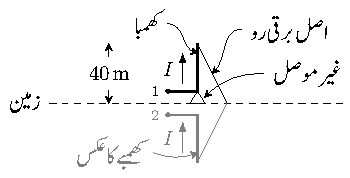
\includegraphics{figAntennaMastAndItsImage}
\caption{کھمبا اینٹینا}
\label{شکل_اینٹینا_کھمبا}
\end{figure}
حل:موصل زمین میں کھمبا اینٹینا کا عکس بنتا ہے۔درکار تعدد پر \عددیء{\lambda=\tfrac{c}{f}=\tfrac{3\times 10^{8}}{300000}=\SI{1000}{\meter}} ہے جو کھمبے کی لمبائی سے بہت زیادہ ہے۔یوں اینٹینا اور اس کا عکس بطور مختصر جفت قطب کردار ادا کرتے ہیں۔چونکہ کھمبے کے سر پر موصل چادر نسب نہیں کیا گیا ہے لہٰذا اس کے پورے لمبائی پر برابر برقی رو تصور کرنا غلط ہو گا۔حقیقت میں، جیسے شکل میں وضاحت کی گئی ہے، کھمبے کے کھلے سر پر برقی رو صفر ہو گی جبکہ نچلے سر پر اس کی قیمت زیادہ سے زیادہ ہو گی۔جیسا شکل میں دکھایا گیا ہے، برقی رو بالمقابل لمبائی \عددیء{l}  کا خط تکونی ہے۔یوں اوسطاً برقی رو \عددیء{I_{\text{اوسط}}=\tfrac{I_0}{2}} ہو گی جہاں برقی رو کی زیادہ سے زیادہ قیمت \عددیء{I_0} ہے۔

یوں \عددیء{2\times 40} میٹر  لمبے فرضی جفت قطب کی اخراجی مزاحمت مساوات \حوالہ{مساوات_اینٹینا_اخراجی_مزاحمت_جفت_قطب} سے 
\begin{align*}
80 \pi^2 \left(\frac{2 \times 40}{1000}\right)^2  \left(\frac{0.5 I_0}{I_0} \right)^2=\SI{1.2633}{\ohm}
\end{align*} 
حاصل ہوتی ہے۔یہ مزاحمت حقیقی کھمبے کے سر \عددیء{1} اور عکسی کھمبے کے سر \عددیء{2} کے مابین ہے۔یوں اصل اینٹینا کی اخراجی مزاحمت جو زمین اور \عددیء{1} کے مابین ناپی جائے گی کی قیمت
\begin{align}
R_{\text{اخراجی}}=\frac{0.63165}{2}=\SI{0.63}{\ohm}
\end{align}
ہو گی۔
\انتہا{مثال}
%==============


حقیقی دھات کامل موصل نہیں ہوتے لہٰذا کسی بھی دھات سے بنائے گئے جفت قطب میں توانائی کا ضیاع ہو گا۔موصل کے علاوہ اینٹینا کے ساتھ منسلک ذو برق میں بھی طاقت کا ضیاع ہو گا۔ان ضیاع کو مزاحمت \عددیء{R_{\text{ضیاعی}}} سے ظاہر کیا جا سکتا ہے۔یوں اینٹینا کے برقی سروں پر کل مزاحمت 
\begin{align}
R=R_{\text{اخراجی}}+R_{\text{ضیاعی}}
\end{align}

ہو گی۔مندرجہ بالا مثال میں اگر \عددیء{R_{\text{ضیاعی}}=\SI{0.63}{\ohm}} ہوتا تب اینٹینا کی کارگزاری\فرہنگ{کارگزاری}\حاشیہب{efficiency}\فرہنگ{efficiency} \عددیء{k}
\begin{align}\label{مساوات_اینٹینا_کارگزاری}
k=\frac{\text{\RL{اخراجی طاقت}}}{\text{\RL{داخلی طاقت}}} = \frac{R_{\text{اخراجی}}}{R_{\text{اخراجی}}+R_{\text{ضیاعی}}} \frac{0.63}{0.63+0.63}=\SI{50}{\percent}
\end{align} 
پچاس فی صد ہو گی۔اگر طاقت کا ضیاع بڑھائے بغیر زیادہ لمبائی کا جفت قطب استعمال کیا جائے تو کارگزاری اس سے بہتر کی جا سکتی ہے۔

اینٹینا کو مکمل گھیرتی بند سطح پر مخلوط پوئنٹنگ سمتیہ کا سطحی تکمل لینے سے حقیقی طاقت کے ساتھ ساتھ خیالی طاقت بھی حاصل ہوتا ہے۔حقیقی طاقت اخراجی طاقت کو ظاہر کرتا ہے جبکہ خیالی طاقت  متعامل جزو ہے۔سطح تکمل کی صورت اور مقام کا تکمل کے حقیقی جزو پر کوئی اثر نہیں البتہ خیالی طاقت کا دارومدار سطح کی صورت اور مقام پر ہے۔اینٹینا سے بہت دور خیالی جزو قابل نظر انداز ہوتا ہے جبکہ اینٹینا کے قریب اس جزو کی مقدار بڑھ جاتی ہے۔نہایت پتلی ساخت کے خطی اینٹینا کی صورت میں اگر سطح تکمل کو بالکل سطح اینٹینا کے ساتھ ملا لیا جائے تب حاصل مخلوط طاقت تقسیم \عددیء{I_0^2} رکاوٹ \عددیء{R+jX} دیتا ہے جہاں \عددیء{R} اینٹینا کے اخراجی مزاحمت کو ظاہر کرتا ہے۔

\حصہ{ٹھوس زاویہ}
اگلے حصے میں \اصطلاح{ٹھوس زاویہ}\فرہنگ{ٹھوس زاویہ}\فرہنگ{زاویہ!ٹھوس}\حاشیہب{solid angle}\فرہنگ{solid angle} درکار ہو گا لہٰذا اسے پہلے سمجھتے ہیں۔

شکل \حوالہ{شکل_اینٹینا_ریڈیئن_تعریف}-الف میں رداس \عددیء{r} کے دائرے پر قوس کی لمبائی \عددیء{l} اور  رداس \عددیء{r} کی شرح
\begin{align}\label{مساوات_اینٹینا_ریڈیئن_تعریف}
\theta=\frac{l}{r} \quad \quad (\si{\radian})
\end{align}
 زاویے \عددیء{\theta} دیتی ہے جس کی اکائی \اصطلاح{ریڈیئن}\حاشیہب{radian} \عددیء{(\si{\radian})} ہے۔یوں اکائی رداس کے دائرے پر اکائی لمبی قوس، دائرے کے مرکز پر، ایک ریڈیئن \عددیء{(\SI{1}{\radian})} کا زاویہ بنائے گی۔یہی اکائی ریڈیئن\فرہنگ{ریڈیئن!تعریف}\فرہنگ{زاویہ!ریڈیئن کی تعریف}\فرہنگ{radian!defined} کی تعریف ہے۔چونکہ دائرے کا محیط \عددیء{2\pi r} ہے لہٰذا دائرے کے گرد ایک مکمل چکر \عددیء{2\pi} ریڈیئن  کے زاویے کو ظاہر کرتی ہے۔اگرچہ مساوات \حوالہ{مساوات_اینٹینا_ریڈیئن_تعریف} کے تحت \عددیء{\theta} دراصل بے بُعد مقدار ہے، ہم اس کے باوجود اس کو فرضی اکائی ریڈیئن میں ناپتے ہیں۔یوں \عددیء{x \, \si{\radian}} سے ظاہر ہوتا ہے کہ \عددیء{x} زاویے کی بات کی جا رہی ہے۔

بالکل اسی طرح  رداس \عددیء{r} کے کرہ کی سطح پر کسی بھی رقبہ \عددیء{S} اور کرہ کے رداس کے مربع \عددیء{r^2} کی شرح
\begin{align}\label{مساوات_اینٹینا_ٹھوس_زاویہ_تعریف}
\Omega=\frac{S}{r^2} \quad \quad (\si{\steradian})
\end{align}
ٹھوس زاویہ \عددیء{\Omega} دیتی ہے جسے مربع ریڈیئن یعنی \اصطلاح{سٹریڈیئن}\فرہنگ{سٹریڈیئن}\فرہنگ{زاویہ!سٹریڈیئن}\حاشیہب{steradian}\فرہنگ{steradian}\فرہنگ{angle!steradian} \عددیء{(\si{\steradian})} میں ناپا جاتا ہے۔اکائی رداس کے کرہ پر اکائی رقبہ، کرہ کے مرکز پر، ایک سٹریڈیئن  کا ٹھوس زاویہ بنائے گی۔یہی سٹریڈیئن کی تعریف ہے۔چونکہ کرہ کی سطح \عددیء{4\pi r^2} کے برابر ہے لہٰذا پوری کرہ \عددیء{4\pi} سٹریڈیئن کا ٹھوس زاویہ دیتی ہے۔اگرچہ ٹھوس زاویہ بے بُعد مقدار ہے، ہم اس کے باوجود اس کو فرضی اکائی سٹریڈیئن میں ناپتے ہیں۔یوں مختلف اعداد کی بات کرتے وقت یہ جاننا ممکن ہوتا ہے کہ ٹھوس زاویے کی بات کی جا رہی ہے۔ 
\begin{figure}
\centering
\begin{subfigure}{0.4\textwidth}
\centering
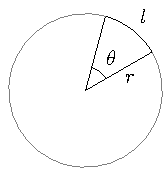
\includegraphics{figAntennaAngleDefinitionRadians}
\caption*{الف: ریڈیئن کی تعریف}
\end{subfigure}%
%
\begin{subfigure}{0.4\textwidth}
\centering
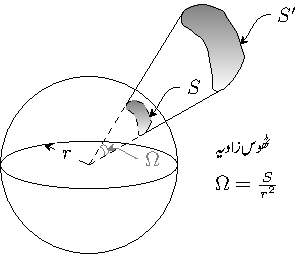
\includegraphics{figAntennaAngleDefinitionSteradians}
\caption*{ب: سٹریڈیئن کی تعریف}
\end{subfigure}%
\caption{ریڈیئن اور سٹریڈیئن کی تعریف}
\label{شکل_اینٹینا_ریڈیئن_تعریف}
\end{figure}

شکل \حوالہ{شکل_اینٹینا_ریڈیئن_تعریف}-ب میں عمومی رقبہ \عددیء{S'} کا محدد کے مرکز پر ٹھوس زاویہ حاصل کرنے کا طریقہ دکھایا گیا ہے۔مرکز سے دیکھتے ہوئے \عددیء{S'} کا بیرونی خاکہ نظر آئے گا۔اگر اس خاکے کے بیرونی کناروں سے  مرکز تک ربڑی چادر کھینچ کر لگائی جائے تو یہ چادر رداس \عددیء{r} کے کرہ کو کاٹے گی۔کرہ کی سطح پر یوں رقبہ \عددیء{S} گھیرا جائے گا۔ٹھوس زاویے
\begin{align}
\Omega=\frac{S}{r^2}
\end{align}
کے برابر ہو گا۔اکائی رداس کے کرہ کی صورت میں رقبہ \عددیء{S} کی قیمت ٹھوس زاویے کی قیمت کے برابر ہو گی۔

شکل \حوالہ{شکل_اینٹینا_ریڈیئن_تعریف}-الف میں \عددیء{\theta}  نظارے کے حدود کو ظاہر کرتا ہے۔اسی طرح شکل \حوالہ{شکل_اینٹینا_ریڈیئن_تعریف}-ب میں \عددیء{\Omega} نظارے  کے حدود تعین کرتا ہے۔

شکل \حوالہ{شکل_اینٹینا_ریڈیئن_تعریف}-الف  میں دکھایا گیا زاویہ سطحی نوعیت کا ہے جسے ریڈیئن میں ناپا جاتا ہے۔اس کے برعکس شکل \حوالہ{شکل_اینٹینا_ریڈیئن_تعریف}-ب  میں دکھایا گیا زاویہ حجمی نوعیت کا ہے جسے سٹریڈیئن یا ریڈیئن کے مربع میں ناپا جاتا ہے۔یاد رہے کہ ایک مربع ریڈیئن کو ہی ایک سٹریڈیئن کہتے ہیں۔
\begin{align}
\SI{1}{\steradian}=\SI{1}{\radian \squared}
\end{align} 

کروی محدد میں \عددیء{r} رداس کے کرہ کی سطح پر رقبے کو
\begin{align}
S=\int_\theta \int_\phi r^2 \sin \theta \dif \theta \dif \phi
\end{align}
لکھا جا سکتا ہے۔یہ رقبہ کرہ کے مرکز پر
\begin{align}
\Omega = \frac{S}{r^2}=\int_\theta \int_\phi \sin \theta \dif \theta \dif \phi \quad \quad (\si{\steradian})
\end{align}
ٹھوس زاویہ بنائے گی۔

\حصہ{اخراجی رقبہ، سمتیت اور افزائش}
مختصر جفت قطب کے دور میدان میں صرف \عددیء{E_\theta} اور \عددیء{H_\phi} پائے جاتے ہیں جنہیں مساوات \حوالہ{مساوات_اینٹینا_جفت_قطب_دور_میدان} میں پیش کیا گیا ہے۔کسی بھی اینٹینا کی طرح اس کے دور میدان \عددیء{\tfrac{1}{r}} کی شرح سے گھٹتے ہیں لہٰذا پوئنٹنگ  سمتیہ
\begin{align}
\pmb{\mathscr{P}}=\frac{1}{2}\left[\kvec{E}_s \times \kvec{H}_s^* \right]_{\text{حقیقی}} =\frac{Z_0}{2} \abs{H}^2 \ar=\frac{1}{2 Z_0}\abs{E}^2 \ar
\end{align} 
\عددیء{\tfrac{1}{r^2}} کی شرح سے گھٹے گی۔یوں پوئنٹنگ  سمتیہ کے رداسی جزو کو \عددیء{r^2} سے ضرب دینے سے \عددیء{P(\theta,\phi)}
\begin{align}
P(\theta,\phi)=r^2 \mathscr{P}=\frac{Z_0}{2} \abs{H}^2 r^2=\frac{1}{2 Z_0}\abs{E}^2 r^2 \quad \quad (\si{\watt / \steradian})
\end{align} 
حاصل ہوتی ہے جس کی قیمت فاصلہ \عددیء{r} بڑھانے سے نہیں گھٹتی۔\عددیء{P(\theta,\phi)} \اصطلاح{اخراجی شدت}\فرہنگ{اخراجی شدت}\فرہنگ{شدت!اخراجی}\حاشیہب{radiation intensity}\فرہنگ{intensity!radiation} کہلاتی ہے۔اخراجی شدت کے بُعد پر غور کریں۔پوئنٹنگ سمتیہ طاقت کی کثافت  یعنی طاقت فی رقبہ دیتی ہے۔مساوات \حوالہ{مساوات_اینٹینا_ٹھوس_زاویہ_تعریف} سے رقبے کو \عددیء{S=\Omega r^2} لکھا جا سکتا ہے۔یوں پوئنٹنگ سمتیہ ضرب مربع رداس کا بُعد طاقت فی ٹھوس زاویہ \عددیء{\si{\watt/\steradian}} بنتی ہے۔ 

اخراجی شدت کو \اصطلاح{تقابل پذیر}\فرہنگ{تقابل پذیر}\حاشیہب{normalized}\فرہنگ{normalized} بنانے کی خاطر \عددیء{P(\theta,\phi)} کو اس کی زیادہ سے زیادہ قیمت \عددیء{P(\theta,\phi)_{\text{بلندتر}}=r^2 \mathscr{P}_{\text{بلندتر}}} سے تقسیم کرتے ہوئے
\begin{align}
P_n(\theta,\phi)=\frac{P(\theta,\phi)}{P(\theta,\phi)_{\text{بلندتر}}} \quad \quad \text{\RL{بے بُعد}}
\end{align}
بے بُعد\فرہنگ{بے بُعد}\حاشیہب{dimensionless} مقدار \عددیء{P_n(\theta,\phi)} حاصل ہوتی ہے جو  اینٹینا کی \اصطلاح{تقابل پذیر نقش طاقت}\فرہنگ{نقش طاقت!تقابل پذیر}\حاشیہب{normalized power pattern}\فرہنگ{power!normalized pattern}  ہے۔

اینٹینا کی کل اخراج
\begin{align}
\int_0^{2\pi}\int_{0}^{\pi} \mathscr{P} r^2 \sin \theta \dif \theta \dif \phi
\end{align}
ہے۔اگر کثافت طاقت \عددیء{\mathscr{P}_{\text{بلندتر}}} ہو تب اتنی اخراج مکمل کرہ کی سطح کے بجائے  کرہ کی سطح پر رقبہ \عددیء{S} سے خارج ہو گی یعنی
\begin{align}
\mathscr{P}_{\text{بلندتر}} S=\int_0^{2\pi}\int_{0}^{\pi} \mathscr{P} r^2 \sin \theta \dif \theta \dif \phi
\end{align}
ہو گا۔اس میں مساوات \حوالہ{مساوات_اینٹینا_ٹھوس_زاویہ_تعریف} کی مدد سے کرہ کی سطح پر رقبے کو ٹھوس زاویے  کی صورت میں لکھتے ہوئے
\begin{align*}
\Omega_A=\int_0^{2\pi}\int_{0}^{\pi} \frac{\mathscr{P} r^2}{\mathscr{P}_{\text{بلندتر}} r^2 } \sin \theta \dif \theta \dif \phi
\end{align*}
یعنی
\begin{align}\label{مساوات_اینٹینا_اخراجی_ٹھوس_زاویہ}
\Omega_A=\int_0^{2\pi}\int_{0}^{\pi} P_n(\theta,\phi) r^2 \sin \theta \dif \theta \dif \phi=\iint \limits_{4\pi} P_n(\theta,\phi) \dif \Omega \quad \quad (\si{\steradian})
\end{align}
حاصل ہوتا ہے۔اس مساوات کے تحت \عددیء{\Omega_A} ٹھوس زاویے پر یکساں زیادہ سے زیادہ طاقت خارج کرتے ہوئے اینٹینا پوری طاقت خارج کر سکتی ہے۔\عددیء{\Omega_A} کو \اصطلاح{اخراجی ٹھوس زاویہ}\فرہنگ{زاویہ!اخراجی ٹھوس}\فرہنگ{اخراجی ٹھوس زاویہ}\حاشیہب{beam solid angle}\فرہنگ{solid angle!beam} کہتے ہیں۔

\اصطلاح{مرکزی شعاع}\فرہنگ{شعاع!مرکزی}\فرہنگ{مرکزی!شعاع}\حاشیہب{main lobe}\فرہنگ{main lobe}\فرہنگ{lobe} پر تکمل
\begin{align}
\Omega_M=\iint \limits_{\text{\RL{مرکزی شعاع}}} P_n(\theta,\phi) \dif \Omega \quad \quad (\si{\steradian})
\end{align}
 لیتے ہوئے \اصطلاح{مرکزی ٹھوس زاویہ}\فرہنگ{ٹھوس!مرکزی زاویہ}\حاشیہب{major lobe solid angle}\فرہنگ{solid angle!major lobe} حاصل کیا جا سکتا ہے۔یوں \اصطلاح{ثانوی شعاع}\فرہنگ{ثانوی شعاع}\حاشیہب{minor lobe}\فرہنگ{lobe!minor} کے ٹھوس زاویہ \عددیء{\Omega_m} کو اخراجی ٹھوس زاویے اور مرکزی ٹھوس زاویے کے فرق
\begin{align}
\Omega_m=\Omega_A-\Omega_M
\end{align}
سے حاصل کیا جا سکتا ہے۔\اصطلاح{غیر سمتی}\فرہنگ{اینٹینا!غیر سمتی}\حاشیہب{isotropic}\فرہنگ{isotropic} اینٹینا ہر سمت میں برابر اخراج کرتی ہے لہٰذا ہر سمت میں اس کا \عددیء{P_n(\theta,\phi)=1} اور \عددیء{\Omega_A=4\pi} ہو گا۔

اینٹینا کی دوسری اہم خاصیت اس کی \اصطلاح{سمتیت}\فرہنگ{سمتیت}\فرہنگ{اینٹینا!سمتیت}\حاشیہب{directivity}\فرہنگ{directivity} ہے۔اخراجی اینٹینا کی زیادہ سے زیادہ اخراجی شدت اور اوسط اخراجی شدت کی شرح
\begin{align}
D=\frac{\text{\RL{زیادہ سے زیادہ اخراجی شدت}}}{\text{\RL{اوسط اخراجی شدت}}} = \frac{P(\theta,\phi)_{\text{بلندتر}}}{P(\theta,\phi)_{\text{اوسط}}} \quad \quad \text{\RL{بے بُعد}}
\end{align}
 اس کی \اصطلاح{سمتیت} کہلاتی ہے۔کل اخراج \عددیء{W} کو \عددیء{4\pi} سٹریڈیئن سے تقسیم کرنے سے اوسط اخراجی شدت \عددیء{P(\theta,\phi)_{\text{اوسط}}} حاصل ہوتی ہے جبکہ اخراجی شدت \عددیء{P(\theta,\phi)} کا \عددیء{4\pi} سٹریڈیئن پر تکمل لینے سے اینٹینا کی کل اخراج حاصل ہوتی ہے۔یوں
\begin{gather}
\begin{aligned}\label{مساوات_اینٹینا_سمتیت_کی_ایک_اور_مساوات}
D=\frac{P(\theta,\phi)_{\text{بلندتر}}}{W/4\pi}&=\frac{4\pi P(\theta,\phi)_{\text{بلندتر}}}{\iint \limits_{4\pi} P(\theta,\phi) \dif \Omega}\\
&=\frac{4\pi}{\iint \limits_{4\pi} \frac{P(\theta,\phi)}{P(\theta,\phi)_{\text{بلندتر}}} \dif \Omega}\\
&=\frac{4\pi}{\iint \limits_{4\pi} P_n(\theta,\phi) \dif \Omega}
\end{aligned}
\end{gather}
لکھی جا سکتی ہے۔مساوات \حوالہ{مساوات_اینٹینا_اخراجی_ٹھوس_زاویہ} کے ساتھ موازنے کے بعد اسے
\begin{align}\label{مساوات_اینٹینا_سمتیت_ٹھوس_زاویہ_تعلق}
D=\frac{4\pi}{\Omega_A} \quad \quad \text{\RL{بے بُعد}}
\end{align}
لکھا جا سکتا ہے۔یوں اینٹینا کی سمتیت سے مراد، کرہ کا ٹھوس زاویہ \عددیء{4\pi} تقسیم اینٹینا کی اخراجی ٹھوس زاویہ \عددیء{\Omega} ہے۔سمتیت اینٹینا کی ایک منفرد خاصیت ہے۔مخصوص ٹھوس زاویے میں طاقت مرکوز کرنے کی صلاحیت کی ناپ سمتیت ہے۔ سمتیت جتنی زیادہ ہو گی اینٹینا اتنی کم ٹھوس زاویے میں طاقت کو مرکوز کر پائے گا۔

%==================
\ابتدا{مثال}
غیر سمتی اینٹینا کی سمتیت حاصل کریں۔

حل: غیر سمتی اینٹینا ہر سمت میں یکساں اخراج کرتی ہے لہٰذا اس کا \عددیء{P_n(\theta,\phi)=1} اور \عددیء{\Omega_A=1} ہوں گے۔ یوں
\begin{align}
D=\frac{4\pi}{\Omega_A}=1
\end{align}
حاصل ہو گا۔کسی بھی اینٹینا کی یہ کم سے کم ممکنہ سمتیت ہے۔
\انتہا{مثال}
%=================

\ابتدا{مثال}
مختصر جفت قطب کی سمتیت حاصل کریں۔

حل: مساوات \حوالہ{مساوات_اینٹینا_جفت_قطب_دور_میدان} استعمال کرتے ہوئے تقابل پذیر نقش طاقت
\begin{align}
P_n(\theta,\phi)=\frac{H^{2}_{\phi}(\theta,\phi)}{H^{2}_{\phi}(\theta,\phi)_{\text{بلندتر}}}  =\sin^2 \theta
\end{align}
لکھی جا سکتی ہے۔مساوات \حوالہ{مساوات_اینٹینا_اخراجی_ٹھوس_زاویہ} سے
\begin{align}
\Omega_A=\int_0^{2\pi} \int_0^{\pi} \sin^2 \theta \dif \theta \dif \phi=\frac{8\pi}{3} 
\end{align}
اور یوں مساوات  \عددیء{مساوات_اینٹینا_سمتیت_ٹھوس_زاویہ_تعلق} سے
\begin{align}
D=\frac{4\pi}{\Omega}=\frac{3}{2}
\end{align}
حاصل ہوتا ہے۔یوں غیر سمتی اینٹینا کی نسبت سے مختصر جفت قطب کی زیادہ سے زیادہ اخراج \عددیء{\tfrac{3}{2}}  گنا زیادہ ہے۔ 
\انتہا{مثال}
%=============

سمتیت کا دارومدار صرف اور صرف دور میدان کی نقش پر ہے۔اس میں اینٹینا کی کارگزاری شامل نہیں ہے۔اس کے برعکس اینٹینا کی کارگزاری،  اینٹینا کی  افزائش طاقت یا \اصطلاح{افزائش}\فرہنگ{افزائش!اینٹینا}\فرہنگ{اینٹینا!افزائش}\حاشیہب{gain}\فرہنگ{gain}\فرہنگ{antenna!gain} پر اثر انداز ہوتی ہے۔اینٹینا کی افزائش سے مراد
\begin{align}
\text{افزائش} = G = \frac{\text{\RL{آزمائشی اینٹینا کی زیادہ سے زیادہ اخراجی شدت}}}{\text{\RL{حوالہ اینٹینا کی زیادہ سے زیادہ اخراجی شدت}}}
\end{align}
ہے جہاں دونوں اینٹینوں کی داخلی طاقت برابر ہے۔کسی بھی اینٹینا کو بطور حوالہ اینٹینا لیا جا سکتا ہے۔اگر ہم  بے ضیاع، غیر سمتی اینٹینا کو حوالہ تصور کریں تب
\begin{align}
G_0 =\frac{P_m'}{P_0}
\end{align}
ہو گا جہاں
\begin{description}
\جزو{$P_m'$} آزمائشی اینٹینا کی زیادہ سے زیادہ اخراجی شدت،
\جزو{$P_0$} بے ضیاع، غیر سمتی اینٹینا کی اخراجی شدت
\end{description}
ہیں۔یاد رہے کہ غیر سمتی اینٹینا ہر سمت میں یکساں اخراج کرتی ہے لہٰذا اس کی زیادہ سے زیادہ شدت اور اوسط اخراجی شدت برابر ہوتے ہیں۔آزمودہ اینٹینا کی اخراجی شدت \عددیء{P_m'} اور  کامل اینٹینا کی اخراجی شدت \عددیء{P_m} کی شرح اینٹینا کی کارگزاری \عددیء{k} دیتی ہے۔یہ وہی \عددیء{k} ہے جسے مساوات \حوالہ{مساوات_اینٹینا_کارگزاری} میں بھی حاصل کیا گیا۔یوں
\begin{align}
G_0 =\frac{k  P_m}{P_0} = k D
\end{align}
حاصل ہوتا ہے۔یہ مساوات کہتی ہے کہ کسی بھی کامل اینٹینا \عددیء{(k=\SI{100}{\percent})} کی افزائش، کامل غیر سمتی اینٹینا کی نسبت سے، اسی اینٹینا کی سمتیت کے برابر ہوتی ہے۔ غیر کامل \عددیء{k < \SI{100}{\percent}} اینٹینا کی صورت میں افزائش کی قیمت سمتیت سے کم ہو گی۔

سمتیت کی قیمت \عددیء{1} تا \عددیء{\infty} ممکن ہے۔سمتیت کی قیمت  اکائی سے کم نہیں ہو سکتی۔اس کے برعکس افزائش کی قیمت صفر تا لا محدود ممکن ہے۔
\begin{align*}
1 \le &D \le \infty\\
0 \le & G \le \infty \quad \quad \text{\RL{ممکنہ قیمت}}
\end{align*}

\begin{figure}
\centering
\begin{subfigure}{0.4\textwidth}
\centering
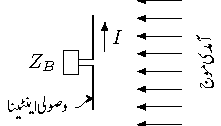
\includegraphics{figAntennaReceivingAntennaToLoad}
\caption*{الف: آمدی موج میں تر وصولی اینٹینا}
\end{subfigure}%
%
\begin{subfigure}{0.4\textwidth}
\centering
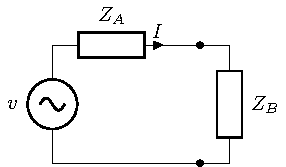
\includegraphics{figAntennaReceivingAntennaToLoadSchematic}
\caption*{ب: اینٹینا کے ساتھ برقی رکاوٹ جوڑا گیا ہے}
\end{subfigure}%
\caption{وصولی اینٹینا آمدی موج سے طاقت حاصل کر کے برقی رکاوٹ کو فراہم کرتی ہے۔}
\label{شکل_اینٹینا_وصولی_اینٹینا_اور_موج}
\end{figure}

\اصطلاح{اخراجی اینٹینا}\فرہنگ{اخراجی!اینٹینا}\فرہنگ{اینٹینا!اخراجی}\حاشیہب{transmitting antenna}\فرہنگ{antenna!transmitting}\فرہنگ{transmitting!antenna} شعاعی اخراج کرتی ہے۔اس کے برعکس \اصطلاح{وصولی اینٹینا}\فرہنگ{وصولی!اینٹینا}\فرہنگ{اینٹینا!وصولی}\حاشیہب{receiving antenna}\فرہنگ{antenna!receiving}\فرہنگ{receiving!antenna} شعاع سے طاقت وصول کرتی ہے۔برقی و مقناطیسی امواج جب وصولی اینٹینا پر پہنچتے ہیں تو وصولی اینٹینا ان سے طاقت حاصل کرتی ہے۔اگر اینٹینا کے برقی سروں پر بیرونی مزاحمت \عددیء{R_B} نسب کی جائے تو حاصل کردہ طاقت کا کچھ حصہ اس مزاحمت میں ضائع ہو گا۔ہم چونکہ بیرونی مزاحمت کو فراہم طاقت \عددیء{W=I^2 R_B} میں دلچسپی رکھتے ہیں لہٰذا اسی کی بات کرتے ہوئے آگے بڑھتے ہیں۔بیرونی مزاحمت کو فراہم طاقت \عددیء{I^2 R_B} کے برابر طاقت آمدی موج کے رقبہ \عددیء{S} میں پایا جاتا ہے۔یوں
\begin{align}
 \mathscr{P} S=I^2 R_B
\end{align} 
لکھا جا سکتا ہے۔ہم فرض کرتے ہیں کہ اینٹینے کا رقبہ \عددیء{S} ہی ہے اور اینٹینا اتنے رقبے پر  آمدی موج سے مکمل طاقت حاصل کرنے اور اسے بیرونی برقی سروں تک منتقل کرنے  کی صلاحیت رکھتی ہے۔اس فرضی رقبے کو \اصطلاح{وصولی رقبہ}\فرہنگ{رقبہ!وصولی}\فرہنگ{اینٹینا!وصولی رقبہ}\حاشیہب{antenna aperture}\فرہنگ{antenna!aperture}\فرہنگ{aperture} کہا جاتا ہے۔یوں وصولی رقبے کو
\begin{align}
S=\frac{I^2 R_B}{\mathscr{P}}
\end{align}
سے حاصل کیا جا سکتا ہے جہاں
\begin{description}
\جزو{$S$} اینٹینا کا فرضی رقبہ، $\si{\meter \squared}$
\جزو{$I$} موثر برقی رو، $\si{\ampere}$
\جزو{$\mathscr{P}$} آمدی موج کا پوئنٹنگ سمتیہ، $\si{\watt /\meter \squared}$
\جزو{$R_L$} برقی مزاحمت، $\si{\ohm}$
\end{description}
ہیں۔حقیقت میں اینٹینا \عددیء{I^2 R_B} سے زیادہ طاقت حاصل کرتی ہے جس کا کچھ حصہ اینٹینا کے اندر ہی ضائع ہو جاتا ہے۔ہمیں اینٹینا کے اندر ضائع ہونے والے طاقت سے کوئی دلچسپی نہیں ہے۔

شکل \حوالہ{شکل_اینٹینا_وصولی_اینٹینا_اور_موج}-الف میں آمدی موج میں تر اینٹینا دکھایا گیا ہے جسے بیرونی برقی رکاوٹ \عددیء{Z_B} کے ساتھ جوڑا گیا ہے۔اینٹینا کا \اصطلاح{تھونن}\فرہنگ{تھونن}\حاشیہب{Thevenin equivalent circuit}\فرہنگ{Thevenin} مساوی دور استعمال کرتے ہوئے،  شکل-ب میں اسی کا  مکمل برقی دور دکھایا گیا ہے۔اس دور میں سلسلہ وار برقی رو
\begin{align*}
I=\frac{v}{Z_A+Z_B}=\frac{v}{R_A+R_B+j(X_A+X_B)}
\end{align*}
ہو گی جہاں
\begin{description}
\جزو{$v$} اینٹینا میں آمدی موج سے پیدا موثر برقی دباو،
\جزو{$R_A$} اینٹینا کے تھونن مساوی دور میں اینٹینا کی مزاحمت،
\جزو{$X_A$} تھونن دور میں اینٹینا کی متعاملیت،
\جزو{$R_B$} بیرونی مزاحمت،
\جزو{$X_B$} بیرونی متعاملیت
\end{description}
ہیں۔یوں بیرونی مزاحمت کو مہیا طاقت 
\begin{align}
\abs{I}^2 R_B=\frac{v^2 R_B}{(R_A+R_B)^2+(X_A+X_B)^2}
\end{align}
ہو گا جس سے  اینٹینے کا رقبہ وصولی
\begin{align}
S=\frac{v^2 R_B}{\mathscr{P}\left[(R_A+R_B)^2+(X_A+X_B)^2\right]}
\end{align}
حاصل ہوتا ہے۔ 

آمدی موج کی نسبت سے ایک مخصوص انداز میں رکھے ہوئے اینٹینا میں زیادہ سے زیادہ برقی دباو پیدا ہو گا۔اسی جگہ اینٹینا کو رکھتے ہوئے بیرونی مزاحمت میں زیادہ سے زیادہ طاقت اس صورت منتقل ہو گی جب
\begin{align}
R_B&=R_A\\
X_B&=-X_A
\end{align}
ہوں۔بے ضیاع اینٹینا کی تھونن مزاحمت دراصل اینٹینا کی اخراجی مزاحمت \عددیء{R_r} ہی ہے۔اس طرح بیرونی مزاحمت میں زیادہ سے زیادہ طاقت منتقل کرتے وقت زیادہ سے زیادہ وصولی رقبہ
\begin{align}\label{مساوات_اینٹینا_اخراجی_رقبہ_اینٹینا}
S_{\text{اخراجی}} = \frac{v^2}{4\mathscr{P} R_r }
\end{align}
 حاصل ہو گا جسے اینٹینا کا \اصطلاح{اخراجی رقبہ}\فرہنگ{اینٹینا!اخراجی رقبہ}\فرہنگ{اخراجی!رقبہ اینٹینا}\حاشیہب{effective aperture}\فرہنگ{effective!aperture} \عددیء{S_{\text{اخراجی}}} پکارا جاتا ہے۔ہر اینٹینا مخصوص قیمت کا \اصطلاح{اخراجی رقبہ} رکھتا ہے۔

%=========================
\ابتدا{مثال}
پورے مختصر جفت قطب پر یکساں برقی رو تصور کرتے ہوئے، اس کا اخراجی رقبہ حاصل کریں۔

حل:مساوات \حوالہ{مساوات_اینٹینا_اخراجی_رقبہ_اینٹینا} سے ظاہر ہے کہ اخراجی رقبہ دریافت کرنے کے لئے، اینٹینا میں پیدا برقی دباو \عددیء{v}، اینٹینا کی اخراجی مزاحمت \عددیء{R_r} اور آمدی موج میں کثافت طاقت \عددیء{\mathscr{P}} درکار ہوں گے۔جفت قطب میں زیادہ سے زیادہ برقی دباو اس صورت پیدا ہو گی جب اینٹینا کی تار اور آمدی موج کا برقی میدان متوازی ہوں۔ایسی صورت میں اینٹینا میں
\begin{align}
v=E l
\end{align}
برقی دباو پیدا ہو گی۔آمدی موج کی پوئنٹنگ سمتیہ
\begin{align}
\mathscr{P}=\frac{E^2}{Z_0} \quad \quad (\si{\watt/ \meter \squared})
\end{align}
ہے جہاں \عددیء{Z_0=\sqrt{\mu_0/\epsilon_0}=120 \pi} خالی خلاء کی قدرتی رکاوٹ ہے۔مساوات \حوالہ{مساوات_اینٹینا_اخراجی_مزاحمت_جفت_قطب} میں \عددیء{I=I_0} پر کرنے سے موجودہ جفت قطب کی اخراجی مزاحمت
\begin{align}
R_r=80 \pi^2 \left(\frac{l}{\lambda}\right)^2
\end{align}
حاصل ہوتی ہے۔ان تمام کو مساوات \حوالہ{مساوات_اینٹینا_اخراجی_رقبہ_اینٹینا} میں پر کرتے ہوئے
\begin{align}
S_{\text{اخراجی}} = \frac{E^2 l^2}{4 \frac{E^2}{Z_0} 80 \pi^2 \left(\frac{l}{\lambda}\right)^2  }=\frac{3\lambda^2}{8\pi}=0.119 \lambda^2 \quad \quad (\si{\meter \squared})
\end{align}
\انتہا{مثال}
%=======================

یوں کامل مختصر جفت قطب کی لمبائی جتنی بھی کم کیوں نہ ہو یہ ہر صورت \عددیء{0.119 \lambda^2} اخراجی رقبے پر آمدی موج سے تمام طاقت حاصل کرنے اور اسے بیرونی مزاحمت تک منتقل کرنے کی صلاحیت رکھتا ہے۔حقیقی جفت قطب غیر کامل ہو گا  لہٰذا اس کی مزاحمت \عددیء{R_{\text{اخراجی}}+R_{\text{ضائع}}} ہو گی۔یوں کامل جفت قطب کا اخراجی رقبہ کچھ کم ہو گا۔

آئیں ایسے اینٹینا کی بات کریں جس کا اخراجی رقبہ \عددیء{S_{\text{اخراجی}}} اور اخراجی ٹھوس زاویہ \عددیء{\Omega_A} ہو۔اخراجی رقبے پر یکساں برقی میدان \عددیء{E_m} کی صورت میں اخراجی طاقت
\begin{align}
P=\frac{E_m^2}{Z} S_{\text{اخراجی}}
\end{align}
ہو گا جہاں \عددیء{Z} انتقالی خطے کی قدرتی رکاوٹ ہے۔

اگر \عددیء{r} فاصلے پر میدان \عددیء{E_r} ہو تب اخراجی طاقت
\begin{align}
P=\frac{E_r^2}{Z} r^2 \Omega_A
\end{align}
ہو گا۔ 

ہم آگے جا کر مساوات \حوالہ{مساوات_اینٹینا_سطحی_دور_میدان_ب} حاصل کریں گے جس کے تحت  \عددیء{E_r=\tfrac{E_m S_{\text{اخراجی}}}{r \lambda}} ہے۔اس نتیجے کو استعمال کرتے ہوئے مندرجہ بالا دو مساوات کو برابر لکھتے ہوئے
\begin{align}\label{مساوات_اینٹینا_اخراجی_ٹھوس_زاویہ_اخراجی_رقبہ_تعلق}
\lambda^2 =S_{\text{اخراجی}} \Omega_A \quad \quad (\si{\meter \squared})
\end{align}
حاصل ہوتا ہے جہاں
\begin{description}
\جزو{$\lambda$} طول موج،
\جزو{$S_{\text{اخراجی}}$}  اینٹینا کا اخراجی رقبہ اور
\جزو{$\Omega_A$} اینٹینا کا اخراجی ٹھوس زاویہ
\end{description}
ہیں۔اس مساوات کے تحت اینٹینا کا اخراجی رقبہ ضرب اخراجی ٹھوس زاویہ برابر ہوتا ہے  طول موج کا مربع۔یوں اگر ہمیں اخراجی رقبہ معلوم ہو تب ہم اخراجی ٹھوس زاویہ حاصل کر سکتے ہیں اور اگر اخراجی ٹھوس زاویہ معلوم ہو تب اخراجی رقبہ حاصل کیا جا سکتا ہے۔

مساوات \حوالہ{مساوات_اینٹینا_سمتیت_ٹھوس_زاویہ_تعلق} میں مساوات \حوالہ{مساوات_اینٹینا_اخراجی_ٹھوس_زاویہ_اخراجی_رقبہ_تعلق} پر کرنے سے
\begin{align}
D=\frac{4\pi}{\lambda^2} S_{\text{اخراجی}}
\end{align}
لکھا جا سکتا ہے۔سمتیت کی یہ تیسری مساوات ہے۔تینوں کو یہاں دوبارہ پیش کرتے ہیں

\begin{gather}
\begin{aligned}\label{مساوات_اینٹینا_سمتیت_مختلف_تعرف}
D&=\frac{P(\theta,\phi)_{\text{بلندتر}}}{P_{\text{اوسط}}} \\
D&=\frac{4\pi}{\Omega} \\
D&=\frac{4\pi}{\lambda^2} S_{\text{اخراجی}}
\end{aligned}
\end{gather}
جہاں پہلی دو مساوات میں سمتیت اخراجی شعاع کے نقش سے حاصل کی گئی ہے جبکہ تیسری مساوات میں اسے اخراجی رقبے سے حاصل کیا گیا ہے۔

\حصہ{قطاری ترتیب}
مسئلہ اینٹینا دراصل اینٹینا کے مختلف حصوں سے پیدا میدانوں کا درست مجموعہ حاصل کرنا ہے۔اینٹینا کے مختلف حصوں کے میدان جمع کرتے ہوئے ان کے انفرادی حیطے اور زاویائی فرق کا خیال رکھنا ضروری ہے۔

\جزوحصہ{غیر سمتی، دو نقطہ منبع}
 دو عدد نقطہ منبع کو شکل میں دکھایا گیا ہے۔دونوں منبع غیر سمتی ہیں اور ان کے درمیان فاصلہ \عددیء{d} ہے۔نقطہ منبع سے مراد ایسی فرضی منبع ہے جس کا حجم صفر کے برابر ہو۔ ہم آگے چل کر \اصطلاح{مسئلہ متکافیت}\فرہنگ{مسئلہ!متکافیت}\فرہنگ{اینٹینا!متکافیت}\حاشیہب{reciprocity}\فرہنگ{reciprocity} دیکھیں گے جس کے تحت نقطہ منبع کے قطاروں کا اخراجی نقش اور انہیں کا وصولی نقش بالکل یکساں ہوتے ہیں۔    

ہم فرض کرتے ہیں کہ دونوں منبع برابر حیطے اور ہم قدم میدان پیدا کرتے ہیں۔دونوں میدان کے خطی تقطیب ہیں۔مزید یہ کہ دونوں کے \عددیء{\kvec{E}} میدان صفحے کے عمودی ہیں۔دونوں منبع سے برابر فاصلے پر ان کے بالکل درمیانے مقام پر زاویائی صفر تصور کرتے ہوئے، دور میدان کو
\begin{align}
E=E_2 e^{j\frac{\psi}{2}} + E_1 e^{-j \frac{\psi}{2}}
\end{align}
لکھا جا سکتا ہے جہاں
\begin{align}
\psi=\beta d \cos \theta=\frac{2\pi d}{\lambda}\cos \theta
\end{align}
ہے۔ان مساوات میں 
\begin{description}
\جزو{$E_1$} منبع-1 کا زاویہ \عددیء{\theta} سمت میں دور میدان،
\جزو{$E_2$} منبع-2 کا زاویہ \عددیء{\theta} سمت میں دور میدان اور
\جزو{$\psi$} دونوں اشارات کا زاویہ \عددیء{\theta} کی سمت میں زاویائی فرق
\end{description}
ہیں۔دونوں دور میدان برابر \عددیء{(E_1=E_2)} ہونے کی صورت میں یوں
\begin{align}\label{مساوات_اینٹینا_دو_نقطہ_الف}
E=E_1 \left(e^{j\frac{\psi}{2}} + e^{-j \frac{\psi}{2}} \right)=2 E_1 \cos \frac{\psi}{2}
\end{align}
ہو گا۔ فاصلہ \عددیء{d=\frac{\lambda}{2}}  کی صورت میں میدان کو شکل میں دکھایا گیا ہے۔

اگر زاویائی صفر کو دونوں منبع کے درمیانے مقام کی جگہ منبع-1 پر چنا جاتا تب دور میدان
\begin{gather}
\begin{aligned}\label{مساوات_اینٹینا_دو_رکنی_قطار}
E&=E_1+E_2 e^{j \psi}\\
&=\left(E_1 e^{-j\frac{\psi}{2}}+E_2 e^{j \frac{\psi}{2}}\right) e^{j\frac{\psi}{2}}
\end{aligned}
\end{gather}
حاصل ہوتا جو \عددیء{E_1=E_2} کی صورت میں 
\begin{align}\label{مساوات_اینٹینا_دو_نقطہ_ب}
E=2 E_1 \cos \frac{\psi}{2} e^{j\frac{\psi}{2}}=2 E_1 \cos \frac{\psi}{2} \phase{\tfrac{\psi}{2}}
\end{align}
حاصل ہوتا۔میدان کا نقش  چونکہ میدان کے حیطے پر منحصر ہوتا ہے لہٰذا اس میں کوئی تبدیلی رونما نہیں ہوئی البتہ میدان کا زاویہ تبدیل ہو گیا ہے۔میدان کے زاویے کی تبدیلی کی وجہ یہ ہے کہ ہم نے زاویے کے صفر کو دونوں منبع کے درمیانے مقام سے ہٹا کر منبع-1 پر چنا ہے۔

\جزوحصہ{ضرب نقش}
گزشتہ حصے میں بالکل یکساں دو عدد غیر سمتی نقطہ منبع کے میدان پر غور کیا گیا۔اگر نقطہ منبع سمتی ہوں  اور دونوں کے نقش بالکل یکساں ہوں تب بھی مساوات \حوالہ{مساوات_اینٹینا_دو_نقطہ_الف} (یا مساوات \حوالہ{مساوات_اینٹینا_دو_نقطہ_ب}) ہی ان کا مجموعی میدان دے گا پس فرق اتنا ہے کہ اب \عددیء{E_1} از خود \عددیء{\theta} کا تفاعل \عددیء{E(\theta)} ہے۔ انفرادی منبع کے نقش \عددیء{E(\theta)} کو \اصطلاح{انفرادی نقش}\فرہنگ{انفرادی نقش}\حاشیہب{primary pattern}\فرہنگ{pattern!primary} جبکہ \عددیء{\cos \tfrac{\psi}{2}} کو  \اصطلاح{قطاری نقش}\فرہنگ{قطار! قطاری نقش}\فرہنگ{نقش!قطاری}\حاشیہب{array pattern}\فرہنگ{pattern!array}\فرہنگ{array!pattern} کہا جائے گا۔یوں
\begin{align}\label{مساوات_اینٹینا_ضرب_نقش}
E=E(\theta) \cos \frac{\psi}{2}
\end{align}
لکھا جا سکتا ہے۔مساوات \حوالہ{مساوات_اینٹینا_ضرب_نقش} \اصطلاح{ضرب نقش}\فرہنگ{نقش!ضرب}\فرہنگ{ضرب نقش}\حاشیہب{pattern multiplication}\فرہنگ{pattern!multiplication} کا اصول بیان کرتا ہے جس کے تحت انفرادی منبع کا نقش اور غیر سمتی نقطہ منبع کے قطار کا نقش ضرب دینے سے سمتی منبع کے قطار کا نقش حاصل ہوتا ہے۔یہاں فرض کیا گیا ہے کہ قطار میں انفرادی نقطہ منبع کا نقش وہی ہے جو اس نقطہ منبع کا تنہائی میں نقش ہوتا ہے۔

\جزوحصہ{ثنائی قطار}
مساوات \حوالہ{مساوات_اینٹینا_دو_نقطہ_ب} دو غیر سمتی زاویائی طور پر ہم قدم نقطہ منبع کے جوڑی کا دور میدان دیتا ہے۔نقطہ منبع کے درمیان فاصلہ \عددیء{\tfrac{\lambda}{2}} اور \عددیء{E_1=\tfrac{1}{2}} ہونے کی صورت میں اس مساوات کو
\begin{align}
E=\cos \left(\frac{\pi}{2}\cos \theta\right)
\end{align}
لکھا جا سکتا ہے۔اس نقش کو شکل میں دکھایا گیا ہے جس میں کوئی ثانوی شعاع نہیں پایا جاتا۔ اس جوڑی منبع کے سیدھ میں \عددیء{\tfrac{\lambda}{2}} فاصلے پر منبع کی دوسری جوڑی رکھنے سے شکل-ب حاصل ہوتا ہے۔اس شکل میں دو درمیانے منبع دراصل ایک ہی نقطے پر پائے جائیں گے لیکن وضاحت کی خاطر انہیں اوپر نیچے دکھایا گیا ہے۔ضرب نقش کے اصول کے تحت ان کا مجموعی میدان
\begin{align}\label{مساوات_اینٹینا_تین_رکنی_قطار}
E=\cos^2 \left(\frac{\pi}{2}\cos \theta\right)
\end{align}
ہو گا جسے شکل میں دکھایا گیا ہے۔اس مساوات پر شق کرنے والوں کے لئے  مثال میں تفصیلی ثبوت پیش کیا گیا ہے۔

اس قطار کو تین عدد منبع کی قطار تصور کیا جا سکتا ہے جہاں قطار میں بالترتیب، منبع کی طاقت \عددیء{(1:2:1)} نسبت سے ہے۔اس تین رکنی قطار کے سیدھ میں لیکن \عددیء{\tfrac{\lambda}{2}} ہٹ کر بالکل ایسی ہی تین رکنی قطار رکھنے سے شکل حاصل ہوتی ہے۔اس نئی قطار کو چار رکنی تصور کیا جا سکتا ہے جہاں بالترتیب منبع کی طاقت \عددیء{(1:3:3:1)} نسبت سے ہے۔ اس چار رکنی قطار کا میدان
\begin{align}
E=\cos^3 \left(\frac{\pi}{2}\cos \theta\right)
\end{align}
ہے۔اس نقش میں بھی ثانوی شعاع نہیں پایا جاتا۔اسی طرح بڑھتے ہوئے، ثانوی شعاع سے پاک، زیادہ سے زیادہ سمتیت کا نقش حاصل کیا جا سکتا ہے۔یوں زیادہ منبع پر مبنی قطار میں منبع کی طاقت \اصطلاح{ثنائی تسلسل}\فرہنگ{ثنائی!تسلسل}\فرہنگ{تسلسل!ثنائی}\حاشیہب{binomial series}\فرہنگ{binomial series} کے \اصطلاح{ثنائی سر}\حاشیہب{binomial coefficient} کی نسبت سے ہوتے ہیں۔ ثنائی سروں کو شکل میں دکھائے گئے \اصطلاح{پاسکل تکون}\فرہنگ{پاسکل تکون}\فرہنگ{تکون!پاسکل}\حاشیہب{Pascal triangle}\فرہنگ{Pascal triangle} کی مدد سے حاصل کیا جا سکتا ہے جس میں ہر اندرونی عدد، اوپر کے قریبی دو اعداد کا مجموعہ ہوتا ہے۔متعدد منبع کے قطار کا نقش
\begin{align}\label{مساوات_اینٹینا_ثنائی_قطار_نقش}
E=\cos^{n-1} \left(\frac{\pi}{2}\cos \theta\right)
\end{align}
کے برابر ہو گا جہاں قطار میں منبع کی تعداد \عددیء{n} ہے۔

اگرچہ مندرجہ بالا \عددیء{n} رکنی  قطار کے نقش میں کوئی ثانوی شعاع نہیں پایا جاتا اس کے باوجود اس کی سمتیت برابر طاقت کے \عددیء{n} رکنی منبع کے قطار سے کم ہوتی ہے۔حقیقی قطار عموماً ان دو صورتوں (ثنائی قطار اور یکساں قطار) کی درمیانی شکل رکھتے ہیں۔  

%====================
\ابتدا{مثال}
مساوات \حوالہ{مساوات_اینٹینا_تین_رکنی_قطار} کو ثابت کریں۔

حل: مساوات \حوالہ{مساوات_اینٹینا_دو_رکنی_قطار} کی طرح زاویائی صفر کو قطار کے پہلی رکن پر چنتے ہوئے
\begin{align*}
E&=E_0+E_0 e^{j\psi}+ E_0 e^{j\psi}+ E_0 e^{j 2\psi}\\
&=E_0 \left(1+e^{j\psi} \right)+E_0 e^{j\psi}\left(1+e^{j\psi} \right)\\
&=E_0 \left(1+e^{j\psi} \right)\left(1+e^{j\psi} \right)\\
&=E_0 \left(1+e^{j\psi} \right)^2
\end{align*}
جس میں \عددیء{E_0=\tfrac{1}{2}} اور \عددیء{\psi=\tfrac{\pi}{2}\cos \theta} پر کرتے ہوئے
\begin{align*}
E&=\left[\left(\frac{e^{-j\frac{\psi}{2}}+e^{j \frac{\psi}{2}}}{2}\right)  e^{j\frac{\psi}{2}} \right]^2=\cos^2 \frac{\psi}{2} \, \phase{\psi}
\end{align*}
لکھا جا سکتا ہے۔اس کا حیطہ \عددیء{\cos^2 \tfrac{\psi}{2}} نقش کی مساوات ہے۔
\انتہا{مثال}
%==============================
\ابتدا{مثال}
مساوات \حوالہ{مساوات_اینٹینا_ثنائی_قطار_نقش} کو تفصیل سے ثابت کریں۔

ثنائی قطار میں رکن کے طاقت ثنائی تسلسل کے سر کی نسبت سے ہوتے ہیں۔یوں \عددیء{n+1} رکنی قطار میں بالترتیب رکن کے طاقت \عددیء{(1+x)^n} کی ثنائی تسلسل
\begin{align}
(1+x)^n =1+\frac{n}{1!}x+\frac{n(n-1)}{2!}x^2+\frac{n(n-1)(n-2)}{3!}x^3+\cdots
\end{align}
  کے سر سے حاصل کئے جاتے ہیں۔یوں تین رکنی قطار کے سر ثنائی تسلسل
\begin{align}
(1+x)^2=1+2x+x^2
\end{align} 
کے سر کی نسبت \عددیء{1:2:1} سے  ہوں گے لہٰذا مندرجہ بالا مساوات میں \عددیء{x=e^{j\psi}} پر کرنے سے تین رکنی قطار کا دور میدان مندرجہ بالا مساوات کے بائیں یا دائیں ہاتھ کی صورت میں لکھا جا سکتا ہے یعنی 
\begin{align}
E=E_0\left(1+e^{j\psi} \right)^2 =E_0 (1+2e^{j\psi} +e^{j 2\psi})
\end{align}
تین رکنی قطار کو دیکھ کر دور میدان مندرجہ بالا مساوات کی دائیں ہاتھ دیتی ہے جسے ثنائی تسلسل کی مدد سے مساوات کی بائیں ہاتھ کی صورت میں بھی لکھا جا سکتا ہے۔مساوات کے بائیں ہاتھ سے نقش \عددیء{\cos^2 \tfrac{\psi}{2}} حاصل ہوتا ہے۔اسی طرح \عددیء{n} رکنی قطار کو \عددیء{(1+x)^{n-1}} کی ثنائی تسلسل کی مدد سے اکھٹے کرتے ہوئے
\begin{align}
E=E_0 \left(1+e^{j\psi} \right)^{n-1}
\end{align}
لکھا جا سکتا ہے جس میں \عددیء{E_0=\tfrac{1}{2}} اور \عددیء{\psi=\pi \cos \theta} پر کرتے ہوئے صرف حیطہ لیتے ہوئے قطار کا نقش
\begin{align}
E=\cos^{n-1} \left(\frac{\pi}{2} \cos \theta\right)
\end{align}
لکھا جا سکتا ہے۔
\انتہا{مثال}
%=====================

\جزوحصہ{یکساں طاقت کے متعدد رکن پر مبنی قطار}
ثنائی قطار غیر یکساں رکنی قطار ہے۔آئیں شکل میں دکھائے گئے \عددیء{n} رکنی، غیر سمتی،  یکساں طاقت کے منبع کی قطار کا دور میدان حاصل کریں۔یہاں فرض کیا جاتا ہے کہ قطار میں ہر دو قریبی منبع میں \عددیء{\delta} زاویائی فرق پایا جاتا ہے۔یوں
\begin{align}
\psi=\beta d \cos \theta +\delta
\end{align}
ہو گا۔قطار  کا دور میدان
\begin{align}\label{مساوات_اینٹینا_یکساں_قطار_الف}
E=E_0\left(1+e^{j \psi}+e^{j 2 \psi}+e^{j 3 \psi} +\cdots +e^{j(n-1)\psi} \right)
\end{align}
لکھا جا سکتا ہے جہاں
\begin{description}
\جزو{$d$} قطار میں رکن کے درمیان فاصلہ،
\جزو{$\delta$} ہر دو قریبی رکن کے درمیان زاویائی فرق اور
\جزو{$\psi$} دو قریبی رکن میں کل زاویائی فرق یعنی \عددیء{\psi=\beta d \cos \theta+\delta}
\end{description}
ہیں۔

اس میں \عددیء{e^{j\psi}=x} پر کرنے سے جانی پہچانی تسلسل
\begin{align*}
E_0 \left(1+x+x^2+x^3+\cdots+x^{n-1}\right)
\end{align*}
حاصل ہوتی ہے جس کا مجموعہ
\begin{align*}
E_0\left(\frac{1-x^{n}}{1-x}\right)
\end{align*}
کے برابر ہے۔

مساوات \حوالہ{مساوات_اینٹینا_یکساں_قطار_الف} کو \عددیء{e^{j\psi}} سے ضرب دیتے ہوئے
\begin{align}\label{مساوات_اینٹینا_یکساں_قطار_ب}
E e^{j\psi}=E_0\left(e^{j \psi}+e^{j 2 \psi}+e^{j 3 \psi} +\cdots +e^{jn\psi} \right)
\end{align}
حاصل ہوتا ہے۔مساوات \حوالہ{مساوات_اینٹینا_یکساں_قطار_الف} سے مساوات \حوالہ{مساوات_اینٹینا_یکساں_قطار_ب} منفی کر کے \عددیء{E} کے لئے حل کرتے  ہوئے
\begin{align}
E=E_0 \frac{1-e^{j n \psi}}{1-e^{j\psi}}=E_0 \frac{\sin \frac{n\psi}{2}}{\sin \frac{\psi}{2}} \, \phase{(n-1)\frac{\lambda}{2}}
\end{align}
حاصل ہوتا ہے۔اگر قطار کے درمیانے نقطے کو زاویائی صفر چنا جاتا تب مندرجہ بالا مساوات میں زاویہ \عددیء{\phase{(n-1)\frac{\lambda}{2}}} نہ پایا جاتا۔تمام رکن غیر سمتی ہونے کی صورت میں \عددیء{E_0} ہر رکن کا انفرادی نقش ہو گا جبکہ \عددیء{\tfrac{\sin \tfrac{n\psi}{2}}{\sin \tfrac{\psi}{2}}} قطاری نقش  ہے۔

غیر سمتی منبع اور زاویائی صفر کا مقام قطار کے درمیانے نقطے پر رکھتے ہوئے 
\begin{align}\label{مساوات_اینٹینا_یکساں_قطار_پ}
E=E_0 \frac{\sin \frac{n\psi}{2}}{\sin \frac{\psi}{2}}
\end{align}
ہو گا۔قطار کی زیادہ سے زیادہ قیمت \عددیء{\psi \to 0} کی صورت میں پائی جائے گی۔چونکہ \عددیء{\psi =0} پر مندرجہ بالا مساوات \عددیء{E=\tfrac{0}{0}} دیتا ہے جو بے معنی\فرہنگ{بے معنی}\حاشیہب{indeterminate}\فرہنگ{indeterminate} ہے لہٰذا ہمیں \اصطلاح{ال ہوس پٹل}\فرہنگ{ال ہوس پٹل}\حاشیہب{L Hospital's rule}\فرہنگ{L Hospital's rule} کا قاعدہ استعمال کرنا ہو گا جس کے تحت اگر تفاعل \عددیء{y=\tfrac{m(x)}{n(x)}} کی قیمت \عددیء{x \to a} پر \عددیء{y=\tfrac{0}{0}} حاصل ہو تب قیمت \عددیء{y=\tfrac{\partial m/\partial x}{\partial n /\partial x}} سے حاصل ہو گی۔یوں مندرجہ بالا مساوات سے \عددیء{\psi \to 0} پر
\begin{align*}
E&=\left. E_0 \frac{\frac{\partial \sin \frac{n\psi}{2}}{\partial \psi}}{\frac{\partial \sin \frac{\psi}{2}}{\partial \psi}}\right|_{\psi \to 0}\\
&=\left. E_0\frac{\frac{n}{2} \cos \frac{n\psi}{2}}{\frac{1}{2} \cos \frac{\psi}{2}}\right|_{\psi \to 0}
\end{align*}
 یعنی
\begin{align}\label{مساوات_اینٹینا_قطار_زیادہ_سے_زیادہ_اخراج}
E=n E_0
\end{align}
حاصل ہوتا ہے جو قطار کی زیادہ سے زیادہ ممکنہ میدان ہے۔یہ میدان قطار میں انفرادی منبع کے طاقت سے \عددیء{n} گنا زیادہ ہے۔ اس قطار کے نقش کی زیادہ سے زیادہ قیمت اس زاویے پر پائی جائے گی جس پر \عددیء{\psi=0} یعنی
\begin{align}\label{مساوات_اینٹینا_بلندتر_اخراج_شرط}
\beta d \cos \theta+\delta=0
\end{align}
ہو جس سے
\begin{align}\label{مساوات_اینٹینا_بلندتر_اخراج_کا_زاویہ}
\theta_{\text{\RL{بلندتر طاقت}}} =\cos^{-1} \left(-\frac{\delta}{\beta d}\right)
\end{align}
حاصل ہوتا ہے۔

اسی طرح اخراجی نقش کا صفر اس مقام پر ہو گا جہاں مساوات \حوالہ{مساوات_اینٹینا_یکساں_قطار_پ} صفر کے برابر ہو یعنی جہاں \عددیء{\tfrac{n \psi}{2}=\mp k \pi} کے برابر ہو یعنی
\begin{align}\label{مساوات_اینٹینا_صفر_کے_مقام_کی_شرط}
\frac{n}{2} \left(\beta d \cos \theta +\delta \right)=\mp k \pi
\end{align}
جس سے صفر اخراج کا زاویہ
\begin{align}
\theta_0 =\cos^{-1} \left[\left(\mp \frac{2 k \pi}{n}-\delta \right)\frac{\lambda}{2\pi d} \right]
\end{align}
حاصل ہوتا ہے جہاں
\begin{description}
\جزو{$\theta_0$} صفر اخراج کا زاویہ،
\جزو{$k$} اعداد \عددیء{k=1,2,3,\cdots} ممکن ہے جہاں \عددیء{k\ne mn} کی شرط لاگو ہے جس میں \عددیء{m=1,2,3,\cdots} کے برابر ہے۔ 
\end{description}


مساوات \حوالہ{مساوات_اینٹینا_یکساں_قطار_پ} کو مساوات \حوالہ{مساوات_اینٹینا_قطار_زیادہ_سے_زیادہ_اخراج} سے تقسیم کرتے ہوئے تقابل پذیر میدان \عددیء{E_n}
\begin{align}\label{مساوات_اینٹینا_یکساں_قطار_تقابل_پذیر_میدان}
E_n=\frac{E}{n E_0}=\frac{1}{n}\frac{\sin \frac{n\psi}{2}}{\sin \frac{\psi}{2}}
\end{align}
حاصل ہوتا ہے۔
%===================
\جزوحصہ{یکساں طاقت کے متعدد رکن پر مبنی قطار: چوڑائی جانب اخراجی قطار}
نقش کی چوٹی اس مقام پر پائی جاتی ہے جس پر \عددیء{\beta d \cos \theta=-\delta} ہو۔ قطار کے سیدھ میں کھڑے ہو کر، چوڑائی جانب \عددیء{(\theta=90^{\circ})} زیادہ سے زیادہ اخراج \عددیء{\delta =0} کی صورت میں ہو گا یعنی جب تمام انفرادی منبع ہم قدم ہوں۔ اگر \عددیء{\theta} کی جگہ اس کا \اصطلاح{زاویہ تکملہ}\فرہنگ{زاویہ!تکملہ}\حاشیہب{complementary angle}\فرہنگ{angle!complementary} \عددیء{\gamma} استعمال کیا جائے تب نقش کے صفر
\begin{align}
\gamma_0=\sin^{-1} \left(\mp \frac{k \lambda}{n d} \right)
\end{align}
پر پائے جائیں گے۔لمبی قطار \عددیء{n d \gg k \lambda}  کی صورت میں \عددیء{\gamma_0} کم قیمت کا ہو گا لہٰذا اسے
\begin{align}\label{مساوات_اینٹینا_قطار_صفر_عمومی}
\gamma_0 =\frac{k}{nd  \!/\! \lambda} \approx \frac{k}{L \!/\! \lambda}
\end{align}
لکھا جا سکتا ہے جہاں قطار کی لمبائی \عددیء{L=(n-1)d} ہے۔لمبائی کو \عددیء{n \gg 1} کی صورت میں
\begin{align*}
L&=(n-1)d \approx nd
\end{align*}
لکھا جا سکتا ہے۔مساوات \حوالہ{مساوات_اینٹینا_قطار_صفر_عمومی} میں \عددیء{k=1} پر کرتے ہوئے نقش کا پہلا صفر \عددیء{\gamma_{01}} حاصل ہوتا ہے۔یوں گوشے کے دونوں اطراف پر پہلے  صفروں کے درمیان  نقش کی چوڑائی
\begin{align}\label{مساوات_اینٹینا_چوڑائی_جانب_اخراجی_پہلی_صفر_چوڑائی}
\text{\RL{پہلی صفر چوڑائی}}=\gamma_{01} \approx \frac{2}{L\! /\!\lambda} \,\si{\radian} \, \, =\frac{114.6^{\circ}}{L\!/\!\lambda}
\end{align} 
حاصل ہوتی ہے۔نقش میں زیادہ سے زیادہ طاقت کے زاویے کے دونوں اطراف وہ زاویے پائے جاتے ہیں جن پر طاقت نصف ہوتی ہے۔ان کے درمیان زاویے کو \اصطلاح{نصف طاقت چوڑائی}\فرہنگ{نصف طاقت چوڑائی}\فرہنگ{چوڑائی!نصف طاقت}\فرہنگ{طاقت!نصف طاقت چوڑائی}\حاشیہب{half power beam width, HPBW}\فرہنگ{half power beam width}،\فرہنگ{HPBW} کہتے ہیں۔لمبے یکساں \اصطلاح{چوڑائی جانب اخراجی قطار}\فرہنگ{چوڑائی جانب اخراجی قطار}\فرہنگ{قطار!چوڑائی جانب اخراجی}\حاشیہب{broadside array}\فرہنگ{broadside array} کے نصف طاقت چوڑائی کی قیمت \اصطلاح{پہلی صفر چوڑائی}\فرہنگ{چوڑائی!پہلی صفر}\فرہنگ{صفر!پہلی صفر چوڑائی}\حاشیہب{beam width between first nulls, BWFN}\فرہنگ{beam width between first nulls}\فرہنگ{BWFN} کے تقریباً آدھی ہوتی ہے۔یوں
\begin{align}
\text{\RL{نصف طاقت چوڑائی}} \approx \frac{\text{\RL{پہلی صفر چوڑائی}}}{2} =\frac{1}{L\!/\!\lambda} \, \si{\radian} \, \, =\frac{57.3^{\circ}}{L \!/\!\lambda}
\end{align}
ہو گی۔

شکل \حوالہ{شکل_اینٹینا_چوڑائی_جانب_اخراجی_قطار} میں چوڑائی جانب اخراجی قطار  کا تقابل پذیر نقش دکھایا گیا ہے۔یہ نقش مساوات \حوالہ{مساوات_اینٹینا_یکساں_قطار_تقابل_پذیر_میدان} سے حاصل کیا گیا ہے۔اس قطار میں منبع \عددیء{\tfrac{\lambda}{2}} فاصلے پر رکھے گئے ہیں۔ بیس عدد برابر طاقت کے منبع پر مبنی اس قطار کی نصف طاقت چوڑائی \عددیء{\theta^{\circ}_{HP}=5.1^{\circ}} ہے۔شکل میں نقش کا تراش دکھایا گیا ہے۔یہ حقیقت میں چرخی مانند ہے لہٰذا
 \عددیء{\phi=0^{\circ}} تا \عددیء{\phi=360^{\circ}} گھومتے ہوئے اس کی صورت یہی نظر آئے گی۔یوں \عددیء{\phi} زاویے پر اس کی نصف طاقت چوڑائی \عددیء{\phi^{\circ}_{HP}=360^{\circ}} ہے۔
\begin{figure}
\centering
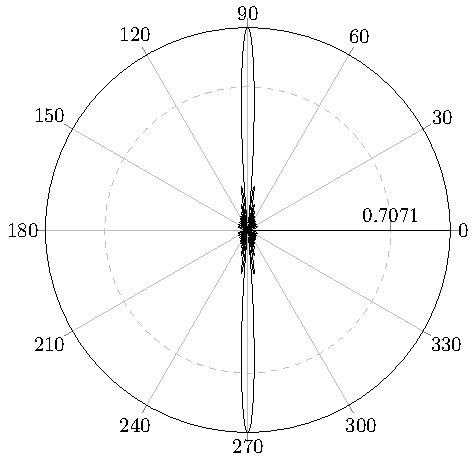
\includegraphics{emtAntennasAndRadiationUniformArrayBroadsideCase}
\caption{چوڑائی جانب اخراجی قطار}
\label{شکل_اینٹینا_چوڑائی_جانب_اخراجی_قطار}
\end{figure}

%=============
\جزوحصہ{یکساں طاقت کے متعدد رکن پر مبنی قطار: لمبائی جانب اخراجی قطار}
زیادہ سے زیادہ اخراج کا زاویہ مساوات \حوالہ{مساوات_اینٹینا_بلندتر_اخراج_شرط}
\begin{align}
\beta d \cos \theta+\delta=0
\end{align}
سے حاصل ہوتا ہے۔قطار کے سیدھ میں کھڑے ہو کر سیدھا آگے \عددیء{(\theta=0)} لمبائی کی جانب  زیادہ سے زیادہ اخراج اس صورت ہو گا جب ہر دو قریبی منبع کے مابین  
\begin{align}
\delta =-\beta d 
\end{align}
زاویائی فرق پایا جاتا ہو۔یوں ایسے قطار کے صفر مساوات \حوالہ{مساوات_اینٹینا_صفر_کے_مقام_کی_شرط} کے تحت
\begin{align*}
\frac{n}{2} \beta d\left( \cos \theta_0 -1 \right)=\mp k \pi
\end{align*}
یعنی
\begin{align*}
 \cos \theta_0 -1=\mp \frac{k}{nd \!/\!\lambda}
\end{align*}
سے حاصل ہوں گے۔اس سے 
\begin{align}
\frac{\theta_0}{2}=\sin^{-1}\left(\mp\sqrt{\frac{k}{2nd \!/\!\lambda}}\right)
\end{align}
لکھا جا سکتا ہے۔لمبی قطار \عددیء{(nd \gg k \lambda)} کی صورت میں اسے
\begin{align}
\theta_0=\mp\sqrt{\frac{2 k}{nd \!/\!\lambda}} \approx \mp \sqrt{\frac{2 k}{L\!/\!\lambda}}
\end{align}
لکھا جا سکتا ہے جہاں لمبائی \عددیء{L=(n-1)d} کو \عددیء{(nd \gg k \lambda)} کی صورت میں \عددیء{L \approx = nd} لکھا گیا ہے۔پہلا صفر \عددیء{k=1} پر حاصل ہو گا جس سے  پہلی صفر چوڑائی
\begin{align}
\text{\RL{پہلی صفر چوڑائی}}= 
2 \theta_{01}  \approx  2 \sqrt{\frac{2}{L\!/\!\lambda}} \, \si{\radian} = 114.6^{\circ} \sqrt{\frac{2}{L\!/\!\lambda}}
\end{align}
حاصل ہوتی ہے۔ 

بیس منبع پر مبنی، لمبائی جانب اخراجی قطار کا تقابل پذیر اخراجی نقش شکل \حوالہ{شکل_اینٹینا_لمبائی_جانب_اخراجی_قطار} میں دکھایا گیا ہے۔یہ نقش مساوات \حوالہ{مساوات_اینٹینا_یکساں_قطار_تقابل_پذیر_میدان} سے حاصل کیا گیا ہے۔منبع کے درمیانی فاصلہ \عددیء{\tfrac{\lambda}{2}} ہے۔مساوات \حوالہ{مساوات_اینٹینا_یکساں_قطار_تقابل_پذیر_میدان} سے پہلی صفر چوڑائی \عددیء{52^{\circ}} اور نصف طاقت چوڑائی \عددیء{\theta^{\circ}_{HP}=34^{\circ}} حاصل ہوتی ہے۔یہ نقش جتنا چوڑا ہے یہ اتنا صفحہ کے عمودی جانب موٹا بھی ہے۔یوں \عددیء{\phi} جانب بھی اس کی نصف طاقت چوڑائی \عددیء{\phi^{\circ}_{HP}=34^{\circ}} ہی ہے۔لمبائی جانب اخراجی لمبی قطار  کی نصف طاقت چوڑائی اس کے پہلے صفر چوڑائی کے تقریباً \عددیء{\tfrac{2}{3}} گنا ہوتی ہے۔ 

\begin{figure}
\centering
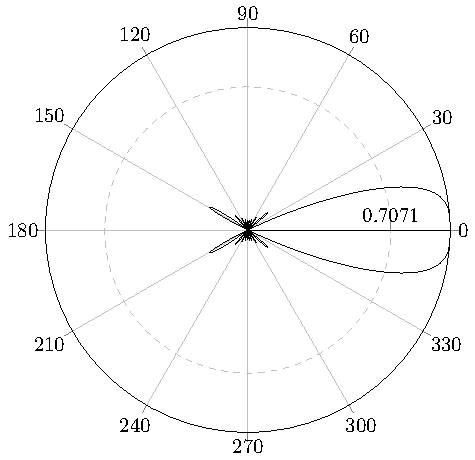
\includegraphics{emtAntennasAndRadiationUniformArrayEndfireCase}
\caption{لمبائی جانب اخراجی قطار}
\label{شکل_اینٹینا_لمبائی_جانب_اخراجی_قطار}
\end{figure}

جیسے مثال \حوالہ{مثال_اینٹینا_چوڑائی_جانب_اخراجی_سمتیت} اور مثال \حوالہ{مثال_اینٹینا_لمبائی_جانب_اخراجی_سمتیت} میں آپ دیکھیں گے کہ \عددیء{n} عدد منبع پر مبنی لمبائی جانب اخراجی قطار کی سمتیت \عددیء{n} عدد منبع پر مبنی چوڑائی جانب اخراجی قطار کی سمتیت سے زیادہ ہوتی ہے۔

مساوات \حوالہ{مساوات_اینٹینا_سمتیت_ٹھوس_زاویہ_تعلق} اینٹینا کی سمتیت 
\begin{align}
D=\frac{4\pi}{\Omega_A} 
\end{align}
دیتا ہے  جہاں ٹھوس زاویہ مساوات \حوالہ{مساوات_اینٹینا_اخراجی_ٹھوس_زاویہ} سے حاصل ہوتا ہے۔اگر ثانوی شعاعوں کو نظرانداز کیا جائے تب مرکزی شعاع کے \عددیء{\theta} سمت میں  نصف طاقت زاویے \عددیء{\theta_{HP}} اور \عددیء{\phi} سمت میں نصف طاقت زاویے \عددیء{\phi_{HP}}  کا ضرب تقریباً ٹھوس زاویے کے برابر ہو گا لہٰذا ایسی صورت میں مساوات \حوالہ{مساوات_اینٹینا_اخراجی_ٹھوس_زاویہ} حل کرنا ضروری نہیں اور  سمتیت کو
\begin{align}\label{مساوات_اینٹینا_قطار_سمتیت_الف}
D \approx \frac{4\pi}{\phi_{HP} \phi_{HP}}
\end{align}
لکھا جا سکتا ہے جہاں نصف طاقت زاویے ریڈیئن میں ہیں۔اس مساوات میں
\begin{align*}
4\pi \, \si{\steradian} = 4 \pi \, \si{\radian^2} =4 \pi \left(\frac{180}{\pi} \right)^2 \, \, \si{deg^2}=\num{41253} \, \si{deg^2}
\end{align*}
پر کرتے ہوئے 
\begin{align}\label{مساوات_اینٹینا_قطار_سمتیت_ب}
D \approx \frac{\num{41253}}{\theta^{\circ}_{HP}\phi^{\circ}_{HP}}
\end{align}
بھی لکھا جا سکتا ہے۔

%================
\ابتدا{مثال}\شناخت{مثال_اینٹینا_چوڑائی_جانب_اخراجی_سمتیت}
بیس رکنی، چوڑائی جانب اخراجی قطار جس میں ارکان \عددیء{\tfrac{\lambda}{2}} فاصلے پر ہیں کے نصف طاقت زاویے \عددیء{\theta^{\circ}_{HP}=5.1^{\circ}} اور \عددیء{\phi^{\circ}_{HP}=360^{\circ}} ہیں کی سمتیت حاصل کریں۔

حل: مساوات \حوالہ{مساوات_اینٹینا_قطار_سمتیت_ب} سے 
\begin{align*}
D \approx \frac{\num{41253}}{5.1 \times 360}=22.5
\end{align*}
حاصل ہوتی ہے۔
\انتہا{مثال}


%================
\ابتدا{مثال}\شناخت{مثال_اینٹینا_لمبائی_جانب_اخراجی_سمتیت}
بیس رکنی، لمبائی جانب اخراجی قطار جس میں ارکان \عددیء{\tfrac{\lambda}{2}} فاصلے پر ہیں کے نصف طاقت زاویے \عددیء{\theta^{\circ}_{HP}=\phi^{\circ}_{HP}=34^{\circ}} ہیں کی سمتیت حاصل کریں۔

حل: مساوات \حوالہ{مساوات_اینٹینا_قطار_سمتیت_ب} سے 
\begin{align*}
D \approx \frac{\num{41253}}{34 \times 34}=35.7
\end{align*}
حاصل ہوتی ہے۔
\انتہا{مثال}
%===============
\ابتدا{مثال}
دو ارکان پر مبنی قطار میں ارکان کے درمیان فاصلہ \عددیء{\tfrac{\lambda}{4}} ہے۔ دائیں رکن (دوسرا رکن) کو \عددیء{90^{\circ}} پیچھے برقی رو مہیا کی گئی ہے۔دونوں برقی رو کی حتمی قیمت برابر ہے۔دونوں ارکان افقی سطح پر سیدھے کھڑے ہیں۔افقی میدان پر اخراجی نقش حاصل کریں۔
   
\begin{figure}
\centering
\begin{subfigure}{0.4\textwidth}
\centering
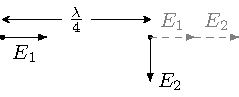
\includegraphics{emtAntennasAndRadiationBroadcastStationLayout}
\caption*{الف: دو رکنی نشریاتی قطار}
\end{subfigure}%
%
\begin{subfigure}{0.4\textwidth}
\centering
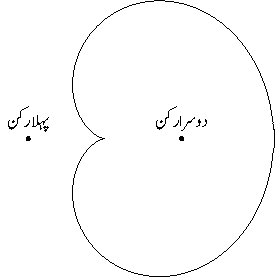
\includegraphics{emtAntennasAndRadiationBroadcastStationExample}
\caption*{دو رکنی قطار کا نقش}
\end{subfigure}%
\caption{دو رکنی اشاعتی قطار اور اس کا نقش}
\label{شکل_اینٹینا_اشاعتی_قطار}
\end{figure}

حل:برقی رو کی حتمی قیمت برابر ہونے کی صورت میں \عددیء{\abs{E_1}=\abs{E_2}=E} ہوں گے۔اگر لمحہ \عددیء{t=0} پر بائیں رکن (پہلا رکن) کا برقی میدان \عددیء{0^{\circ}} میکانی زاویے پر ہو تب اسی لمحہ دائیں رکن (دوسرا رکن) کا میدان \عددیء{-90^{\circ}} میکانی زاویے پر ہو گا۔شکل \حوالہ{شکل_اینٹینا_اشاعتی_قطار}-الف میں ان میدان (\عددیء{E_1} اور \عددیء{E_2}) کو گاڑھی سیاہی میں دکھایا گیا ہے۔ چونکہ دونوں ارکان میں \عددیء{\tfrac{\lambda}{4}} کا فاصلہ ہے لہٰذا جتنی دیر میں بائیں رکن کے میدان کی موج \عددیء{E_1} چل کر دائیں رکن تک پہنچے گا اتنی دیر میں دوری عرصے کے \عددیء{\tfrac{1}{4}} برابر وقت گزر چکا ہو گا لہٰذا دوسرے رکن میں برقی رو \عددیء{\tfrac{1}{4} \times 360^{\circ}=90^{\circ}} آگے بڑھ چکی ہو گی اور یوں اس لمحہ پر دوسرا رکن \عددیء{0^{\circ}} میکانی زاویے پر ہی میدان پیدا کرے گا۔یوں دوسرے رکن کے مقام پر دونوں میدان ہم قدم پائے جائیں گے لہٰذا یہاں برقی میدان \عددیء{E_1+E_2} یعنی دگنا ہو گا۔شکل \حوالہ{شکل_اینٹینا_اشاعتی_قطار}-الف میں کچھ دیر بعد کے ان میدان کو ہلکی سیاہی میں ہم قدم دکھایا گیا ہے۔دونوں میدان دائیں جانب ہم قدم رہتے ہوئے حرکت کریں گے۔

اس کے برعکس جس لمحہ دائیں رکن کی برقی رو  \عددیء{0^{\circ}} پر ہو اسی لمحہ بائیں رکن کی برقی رو \عددیء{90^{\circ}} پر ہو گی۔اس لمحے پر دائیں رکن کا میدان \عددیء{0^{\circ}} پر ہو گا جبکہ بائیں رکن کا میدان \عددیء{90^{\circ}} پر ہو گا۔اب جتنی دیر میں دائیں رکن کا میدان بائیں رکن تک پہنچے گا اتنی دیر میں دائیں رکن کا میدان مزید \عددیء{90^{\circ}} آگے بڑھ کر \عددیء{180^{\circ}} پر پہنچ چکا ہو گا۔یوں دائیں رکن کے مقام پر دونوں میدان آپس میں الٹ سمت میں ہوں گے لہٰذا ان کا مجموعہ صفر کے برابر ہو گا۔اس طرح دائیں رکن کے دائیں جانب میدان صفر ہی پایا جائے گا۔شکل \حوالہ{شکل_اینٹینا_اشاعتی_قطار} میں صفر اور پائے ریڈیئن زاویوں  پر دگنا اور صفر میدان دکھایا گیا ہے۔ 

دونوں رکن کے درمیان عمودی لکیر پر پہنچنے کے لئے دونوں میدان کو برابر دورانیے کی ضرورت ہے لہٰذا اس لکیر پر دونوں میدان آپس میں عمودی رہیں گے۔یوں اس لکیر پر کل میدان مسئلہ فیثاغورث کی مدد سے \عددیء{\sqrt{E^2+E^2}=1.4142E} حاصل ہو گا۔شکل \حوالہ{شکل_اینٹینا_اشاعتی_قطار}-ب میں اسی طرح مختلف مقامات پر میدان حاصل کرتے ہوئے حاصل کردہ نقش دکھایا گیا ہے۔
\انتہا{مثال}
%=========================

مندرجہ بالا مثال کے نقش سے ظاہر ہے کہ یہ اینٹینا بائیں جانب اخراج نہیں کرتا لہٰذا اس کے بائیں جانب دوسرا اینٹینا نسب کیا جا سکتا ہے جس کی اخراجی سمت بائیں رکھی جائے گی تا کہ دونوں علیحدہ علیحدہ نشریات کر سکیں۔  

\جزوحصہ{یکساں طاقت کے متعدد رکن پر مبنی قطار: بدلتے زاویہ اخراجی اینٹینا}
مساوات \حوالہ{مساوات_اینٹینا_بلندتر_اخراج_کا_زاویہ}
\begin{align}
\theta_{\text{\RL{بلندتر طاقت}}} =\cos^{-1} \left(-\frac{\delta}{\beta d}\right)
\end{align}
یکساں ارکان کے قطار کی مرکزی نقش کا زاویہ دیتی ہے۔چوڑائی جانب اخراجی قطار میں \عددیء{\theta=90^{\circ}} رکھا جاتا ہے جبکہ لمبائی جانب اخراجی قطار میں \عددیء{\theta=0^{\circ}} رکھا جاتا ہے۔اگر شعاع کی سمت تبدیل کرنی ہو تو ایسے اینٹینا کو گھمانا ہو گا۔

مساوات \حوالہ{مساوات_اینٹینا_بلندتر_اخراج_کا_زاویہ} کے تحت \عددیء{\delta} کو تبدیل کرتے ہوئے شعاع کی سمت کسی بھی زاویے پر رکھی جا سکتی ہے۔یوں \عددیء{\delta} کو \عددیء{-1} تا \عددیء{+1} مسلسل تبدیل کرتے ہوئے شعاع کی سمت کو \عددیء{0^{\circ}} تا \عددیء{180^{\circ}} مسلسل تبدیل کیا جا سکتا ہے۔یوں \اصطلاح{بدلتے زاویہ اخراجی اینٹینا}\فرہنگ{بدلتے زاویہ اخراجی اینٹینا}\فرہنگ{اینٹینا!بدلتا زاویہ}\حاشیہب{scanning antenna}\فرہنگ{scanning antenna} کو ہلائے بغیر اس کی اخراجی سمت تبدیل کی جا سکتی ہے۔

\حصہ{تداخُل پیما}
\اصطلاح{فلکیات}\فرہنگ{فلکیات}\حاشیہب{astronomy}\فرہنگ{astronomy} کے میدان میں اینٹینا کا کلیدی کردار ہے۔ریڈیائی فلکیات\فرہنگ{ریڈیائی!فلکیات}\حاشیہب{radio astronomy}\فرہنگ{radio!astronomy} میں استعمال ہونے والے اینٹینا کو \اصطلاح{تداخل پیما}\فرہنگ{تداخل پیما}\حاشیہب{interferometer}\فرہنگ{interferometer} اینٹینا کہتے ہیں۔
\begin{figure}
\centering
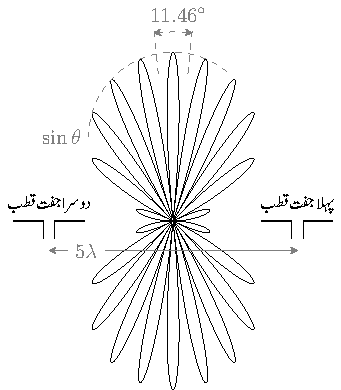
\includegraphics{emtAntennasAndRadiationInterferometer}
\caption{دو عدد مختصر جفت قطب جنہیں \عددیء{5 \lambda} فاصلے پر رکھا گیا ہے سے حاصل تداخل پیما کا نقش۔}
\label{شکل_اینٹینا_تداخل_پیما}
\end{figure}

شکل \حوالہ{شکل_اینٹینا_تداخل_پیما} میں دو عدد مختصر جفت قطب کے درمیان فاصلہ \عددیء{L} ہے۔دونوں کو ہم قدم برقی رو مہیا کی گئی ہے۔ضرب نقش کی ترکیب استعمال کرتے ہوئے اس کا نقش
\begin{align}
E=2 E_1 \cos \frac{\psi}{2}
\end{align}
لکھا جا سکتا ہے جہاں \عددیء{\psi=\beta L \cos \theta} کے برابر ہے۔ضرب نقش کے تحت \عددیء{E_1} انفرادی رکن کی نقش ہے جبکہ \عددیء{\cos \tfrac{\psi}{2}}  دو رکنی قطار کا نقش ہے۔ہمیں میدان بالمقابل زاویہ سے غرض ہے۔مساوات \حوالہ{مساوات_اینٹینا_مختصر_جفت_قطب_عمومی_اینٹینا} مختصر جفت قطب کا نقش دیتا ہے  جس میں میدان اور زاویے کا تعلق \عددیء{\sin \theta}  ہے۔اسی کو استعمال کرتے ہوئے  تقابل پذیر نقش
\begin{align}
E=\sin \theta \cos \frac{\psi}{2}=\sin \theta \cos \left(\frac{\pi L }{\lambda}\cos \theta \right)
\end{align}
لکھا جا سکتا ہے جہاں \عددیء{\beta=\tfrac{2\pi}{\lambda}} کا استعمال کیا گیا ہے۔شکل \حوالہ{شکل_اینٹینا_تداخل_پیما} میں \عددیء{L=5\lambda} کے لئے نقش دکھایا گیا ہے۔زاویہ \عددیء{\theta}  کا زاویہ تکملہ \عددیء{\gamma=\tfrac{\pi}{2}-\theta} استعمال کرتے ہوئے، پہلا صفر
\begin{align*}
\frac{\pi L }{\lambda}\cos \theta =\frac{\pi L }{\lambda}\sin \gamma_{01}=\frac{\pi}{2}
\end{align*}
کی صورت میں پایا جائے گا جس سے 
\begin{align}
\gamma_{01}=\sin^{-1} \frac{1}{2 L \!/\!\lambda}
\end{align}
حاصل ہوتا ہے۔اگر \عددیء{L \gg \lambda} ہو تب پہلی صفر چوڑائی
\begin{align}\label{مساوات_اینٹینا_صفر_چوڑائی_فلکیات}
\text{\RL{پہلی صفر چوڑائی}}= 2 \gamma_{01} = \frac{1}{L\!/\!\lambda} \, \si{\radian} =\frac{57.3}{L\!/\!\lambda} \,\si{deg}
\end{align}
لکھی جا سکتی ہے۔یہ مساوات \حوالہ{مساوات_اینٹینا_چوڑائی_جانب_اخراجی_پہلی_صفر_چوڑائی} میں دیے، \عددیء{n} رکنی چوڑائی جانب اخراجی قطار کے پہلی صفر چوڑائی کی آدھی قیمت ہے۔ہلکی سیاہی کے نقطہ دار لکیر سے شکل میں مختصر جفت قطب کے نقش \عددیء{\sin \theta} کو واضح کیا گیا ہے۔

پانچ طول موج برابر \عددیء{L} کی صورت میں مساوات \حوالہ{مساوات_اینٹینا_صفر_چوڑائی_فلکیات} سے پہلی صفر چوڑائی \عددیء{11.46^{\circ}} حاصل ہوتی ہے۔ 

ریڈیائی فلکیات میں فلکی اخراجی مادے کی شعاع کو  تداخل پیما سے  وصول کیا جاتا ہے۔ان کی جسامت کا بہتر سے بہتر تخمینہ لگانے میں چوڑائی نقش کردار ادا کرتی ہے۔
%=====================
\ابتدا{مشق}
\عددیء{L=20\lambda} کی صورت میں تداخل پیما کی پہلی صفر چوڑائی حاصل کریں۔

جواب:\عددیء{2.865^{\circ}}
\انتہا{مشق}
%=========================

\حصہ{مستطیل سطحی اینٹینا}
ہم متعدد تعداد کے نقطہ منبع پر مبنی مختلف اقسام کے اینٹینا دیکھ چکے ہیں۔اگر نقطہ منبع کے صف در صف اتنے قریب قریب فرضی سطح پر رکھے جائیں کہ یہ علیحدہ علیحدہ منبع کی جگہ ایک مسلسل سطح نظر آئے تو ایسی صورت میں \اصطلاح{سطحی اینٹینا}\فرہنگ{سطحی اینٹینا}\حاشیہب{continuous aperture}\فرہنگ{continuous aperture} حاصل ہو گا۔ایسی ہی ایک مستطیلی سطح جس کی \عددیء{x} سمت میں لمبائی \عددیء{x_1} اور \عددیء{y} سمت میں لمبائی \عددیء{a} ہے کو شکل \حوالہ{شکل_اینٹینا_مستطیل_سطحی} میں دکھایا گیا ہے۔تصور کریں کہ اس سطح پر \عددی{J_x} کثافت برقی رو پائی جاتی ہے۔یہ تصور کرتے ہوئے کہ سطح کے نیچے یعنی \عددی{z<0} خطے میں مقناطیسی میدان نہیں پایا جاتا، ایمپیئر کے دوری قانون کی مدد سے 
\begin{align}\label{مساوات_اینٹینا_فرضی_کثافت_رو}
H_y=-J_x
\end{align}
لکھا جا سکتا ہے جہاں \عددی{H_y} سطح کے انتہائی قریب بالائی جانب\حاشیہد{یہاں فرض کیا گیا ہے کہ سطحی اینٹینا نچلی جانب اخراج نہیں کر رہی۔اگر اینٹینا نچلی جانب بھی اخراج کرے تب \عددی{H_y=-0.5 J_x} لکھا جائے گا۔} مقناطیسی میدان ہے۔سطحی اینٹینا کے دور میدان پر تبصرے سے پہلے ایک حقیقت پر غور کرتے ہیں۔

\begin{figure}
\centering
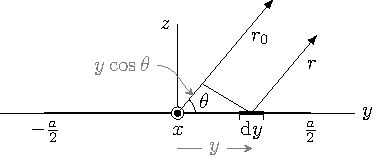
\includegraphics{emtAntennasAndRadiationContinuousApertureA}
\caption{مستطیل سطحی اینٹینا}
\label{شکل_اینٹینا_مستطیل_سطحی}
\end{figure}

فرض کریں کی خالی خلاء میں سطحی برقی و مقناطیسی موج پائی جاتی ہے۔\اصطلاح{ہائی گن}\فرہنگ{ہائی گن}\حاشیہب{Huygen's principle}\فرہنگ{Huygen's principle} کے اصول کے تحت محاذ موج پر ہر نقطہ، منبع موج کا کردار ادا کرتا ہے۔یوں سطح پر چھوٹے رقبے  \عددیء{\dif x \dif y} پر خطی قطبی برقی میدان \عددیء{E_x} بطور منبع کردار ادا کرے گا۔سطح کے برقی میدان \عددیء{E_x} سے یہاں کا مقناطیسی میدان
\begin{align}\label{مساوات_اینٹینا_فرضی_مقناطیسی_میدان}
H_y=\frac{E_x}{Z_0}
\end{align}
لکھا جا سکتا ہے جہاں \عددیء{Z_0} خطے کی قدرتی رکاوٹ \عددیء{\sqrt{\tfrac{\mu_0}{\epsilon_0}}} ہے۔

مساوات \حوالہ{مساوات_اینٹینا_فرضی_کثافت_رو} اور مساوات \حوالہ{مساوات_اینٹینا_فرضی_مقناطیسی_میدان} دو مختلف وجوہات کی بنا پر پیدا مقناطیسی میدان ظاہر کرتے ہیں۔دور سے ان دونوں میں کسی قسم کا کوئی فرق نہیں دیکھا جا سکتا لہٰذا ان دونوں سے پیدا موج میں بھی کوئی فرق نہیں پایا جائے گا۔اس حقیقت کو مد نظر رکھتے ہوئے  آپ دیکھ سکتے ہیں کہ سطحی اینٹینا کا دور میدان اور  خلاء میں فرضی سطح پر موج کا دور میدان بالکل یکساں ہوں گے۔اس حقیقت کو استعمال کرتے ہوئے کسی بھی سطح پر کثافت برقی رو \عددی{J_x} کو خالی خلاء میں مقناطیسی میدان \عددی{H_y} یا برقی میدان \عددی{E_x} سے ظاہر کیا جا سکتا ہے۔
\begin{align}\label{مساوات_اینٹینا_حقیقی_اور_فرضی}
-J_x=H_y=\frac{E_x}{Z_0}
\end{align}
اس طرح مندرجہ ذیل تبصرہ ان دونوں کے لئے قابل قبول ہے۔

آئیں اب واپس اصل موضوع پر آتے ہیں۔تصور کریں کہ شکل \حوالہ{شکل_اینٹینا_مستطیل_سطحی} کے سطحی اینٹینا پر \عددی{x} سمت میں نہ تبدیل ہوتی جبکہ \عددی{y} سمت میں تبدیل ہوتی کثافت برقی رو \عددی{J_x(y)} پائی جاتی ہے۔پوری سطح پر کثافت برقی رو ہم قدم ہے۔

مساوات \حوالہ{مساوات_اینٹینا_جفت_قطب_سمتی_دباو_حاصل} میں \عددیء{I_0=J_x  \dif y} اور \عددیء{\dif l=\dif x} پر کرنے  سے \عددیء{A} حاصل کرتے ہوئے، چھوٹے رقبے  \عددیء{\dif x \dif y} سے دور تفرق میدان کو \عددیء{E=-j\omega A} سے حاصل کیا جا سکتا ہے یعنی
\begin{gather}
\begin{aligned}
\dif E &=-j \omega [\dif A_x] \\
&=-j \omega \frac{\mu_0 I_0 \dif l \, e^{j(\omega t -\beta r)}}{4\pi r}  \\
&=-j \omega \frac{\mu_0 J_x \dif y \dif x \, e^{j(\omega t -\beta r)}}{4\pi r}  \\
&=\frac{j \omega \mu_0 E(y)}{4\pi r Z_0} e^{j(\omega t-\beta r)} \dif x \dif y
\end{aligned}
\end{gather}
جہاں مساوات \حوالہ{مساوات_اینٹینا_حقیقی_اور_فرضی} کا سہارا لیا گیا ہے۔پورے رقبے  سے پیدا میدان سطحی تکمل سے حاصل ہو گا۔رقبے کے وسط سے \عددیء{r_0} فاصلے اور \عددیء{\theta} زاویے پر میدان
\begin{align}
E(\theta)=\frac{j \omega \mu_0 e^{j(\omega t-\beta r_0)}}{4\pi r_0 Z_0} \int \limits_{^{-a}\!/\!_2}^{^a\!/\!_2} \int \limits_{^{-x_1}\!/\!_2}^{^{x_1}\!/\!_2} E(y) e^{j\beta y \cos \theta} \dif x \dif y
\end{align}
ہو گا جہاں \عددیء{r \approx r_0} لیا\حاشیہد{جیسے حصہ \حوالہ{حصہ_اینٹینا_تکمل} میں دکھایا گیا ہے۔} گیا ہے۔بیرونی تکمل لیتے اور \عددیء{\tfrac{\omega \mu_0}{4\pi Z_0}=\tfrac{1}{2\lambda}} پر کرتے ہوئے  میدان کی حتمی قیمت \عددیء{\abs{E}} 
\begin{align}\label{مساوات_اینٹینا_فوریئر_تعلق_الف}
E(\theta)=\frac{x_1}{2 r_0 \lambda} \int \limits_{^{-a}\!/\!_2}^{^a\!/\!_2}  E(y) e^{j\beta y \cos \theta} \dif y
\end{align}
حاصل ہوتی ہے جہاں \عددی{\abs{j e^{(\omega t -\beta r_0)}}=1} لیا گیا ہے۔پوری سطح پر یکساں میدان \عددیء{E(y)=E_a} کی صورت میں
\begin{align}
E(\theta)=\frac{x_1 E_a}{2 r_0 \lambda} \int \limits_{^{-a}\!/\!_2}^{^a\!/\!_2}  e^{j\beta y \cos \theta} \dif y
\end{align}
لکھتے ہوئے
\begin{gather}
\begin{aligned}\label{مساوات_اینٹینا_سطحی_دور_میدان}
E(\theta)&=\frac{x_1 a E_a }{2 r_0 \lambda} \frac{\sin [{(\beta a}\!/\!_2)\cos \theta ]}{({\beta a}\!/\!_2)\cos \theta}\\
&=\frac{E_a S_{\text{اخراجی}}}{2 r_0 \lambda} \frac{\sin [{(\beta a}\!/\!_2)\cos \theta ]}{({\beta a}\!/\!_2)\cos \theta}
\end{aligned}
\end{gather}
حاصل ہو گا جہاں \عددیء{S_{\text{اخراجی}}} سطح کا رقبہ ہے۔

زیادہ سے زیادہ میدان \عددیء{\theta=90^{\circ}} پر 
\begin{align}\label{مساوات_اینٹینا_سطحی_دور_میدان_الف}
E(\theta)_{\text{بلندتر}}=\frac{E_a S_{\text{اخراجی}}}{2 r_0 \lambda} \quad \quad \text{\RL{دو رُخی اخراج}}
\end{align}
حاصل ہوتا ہے۔اگر \عددیء{\theta=270^{\circ}} جانب اخراج صفر ہو تب \عددیء{\theta=90^{\circ}} جانب اخراج دگنی
\begin{align}\label{مساوات_اینٹینا_سطحی_دور_میدان_ب}
E(\theta)_{\text{بلندتر}}=\frac{E_a S_{\text{اخراجی}}}{r_0 \lambda} \quad \quad \text{\RL{یک رُخی اخراج}}
\end{align}
 ہو گی۔اس میدان کو \عددیء{a=5\lambda} اور \عددیء{a=\tfrac{\lambda}{2}} کے لئے شکل \حوالہ{شکل_اینٹینا_مستطیل_سطحی_نقش} میں دکھایا گیا ہے۔
\begin{figure}
\centering
\begin{subfigure}{0.4\textwidth}
\centering
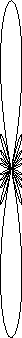
\includegraphics{emtAntennasAndRadiationContinuousApertureB}
\caption*{الف: مستطیل سطحی اینٹینا کا \عددیء{a=5\lambda} کی صورت میں نقش}
\end{subfigure}%
%
\begin{subfigure}{0.4\textwidth}
\centering
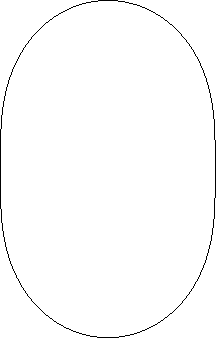
\includegraphics{emtAntennasAndRadiationContinuousApertureC}
\caption*{ب: مستطیل سطحی اینٹینا کا \عددیء{a=\tfrac{\lambda}{2}} کی صورت میں نقش}
\end{subfigure}%
\caption{مستطیل سطح کے نقش}
\label{شکل_اینٹینا_مستطیل_سطحی_نقش}
\end{figure}

صفحہ \حوالہصفحہ{مساوات_اینٹینا_یکساں_قطار_پ} پر مساوات \حوالہ{مساوات_اینٹینا_یکساں_قطار_پ}
\begin{align*}
E(\theta)=E_0 \frac{\sin \frac{n\psi}{2}}{\sin \frac{\psi}{2}}
\end{align*}
یکساں غیر سمتی \عددیء{n} رکنی قطار کا دور میدان دیتی ہے جہاں \عددیء{(\psi=\beta d \cos \theta +\delta)} ہے اور \عددیء{E_0} انفرادی رکن کا میدان ہے۔چوڑائی جانب اخراجی قطار \عددیء{\delta=0} کی صورت میں حاصل ہوتا ہے جس سے مندرجہ بالا مساوات 
\begin{align}\label{مساوات_اینٹینا_چوڑائی_دوبارہ_الف}
E(\theta)=E_0 \frac{\sin [{(n \beta d}\!/\!_2)\cos \theta ]}{\sin [{(\beta d}\!/\!_2)\cos \theta ]}
\end{align}
صورت اختیار کر لیتی ہے۔قطار کی لمبائی \عددیء{a'} لکھتے ہوئے، زیادہ قیمت کی \عددیء{n} اور \عددیء{a'} کی صورت میں \عددیء{a'=(n-1)d\approx nd} ہو گا۔اگر ہم اپنی توجہ \عددیء{\theta=90^{\circ}} کے قریب رکھیں تب مساوات \حوالہ{مساوات_اینٹینا_چوڑائی_دوبارہ_الف} کو 
\begin{align}
E(\theta)= n E_0 \frac{\sin [{( \beta a'}\!/\!_2)\cos \theta ]}{{(\beta a'}\!/\!_2)\cos \theta }
\end{align}
لکھا جا سکتا ہے۔اس مساوات کا مساوات \حوالہ{مساوات_اینٹینا_سطحی_دور_میدان} کے ساتھ موازنہ کرنے سے ہم دیکھتے ہیں کہ \عددیء{a} لمبائی کی سطحی اینٹینا اور \عددیء{n} رکنی \عددیء{a'} لمبی چوڑائی اخراجی قطار  کے مرکزی شعاع ایک جیسے ہیں۔مزید \عددیء{n E_0=\tfrac{E_a S_{\text{اخراجی}}}{2 r_0 \lambda}} کی صورت میں دونوں کے میدان بالکل برابر حتمی قیمت رکھتے ہیں۔

%=============================

\حصہ{درز کا دور میدان بذریعہ فوریئر بدل}
ہم کسی بھی کثافت برقی رو کا پیدا کردہ دور میدان حاصل کرنا دیکھ چکے ہیں۔بعض اوقات ہمیں کثافت برقی رو معلوم نہیں ہوتی البتہ کسی مخصوص سطح پر میدان معلوم ہوتا ہے۔اس طرح کے مسئلے کی مثال مستطیل پیپا اینٹینا ہے۔مستطیل مویج کا منہ کھول کر مستطیل پیپا اینٹینا حاصل کیا جاتا ہے۔اس اینٹینا کے منہ پر کسی قسم کی موصل چادر نہیں نسب کی جاتی لہٰذا اس کے کھلے منہ کے کناروں پر برقی رو پائی جاتی ہے جس کی شکل جاننا دشوار ہے۔البتہ پیپے کی منہ پر برقی میدان جاننا نسبتاً آسان کام ہے۔ہم دیکھیں گے کہ ایسی صورت میں دور میدان قریبی میدان کے \اصطلاح{فوریئر بدل}\فرہنگ{فوریئر بدل!جوڑی}\حاشیہب{Fourier transform pair}\فرہنگ{Fourier transform!pair}  سے حاصل ہوتا ہے۔ آئیں پہلے فوریئر بدل کی یاد دوبارہ تازہ کریں۔
 
آپ فوریئر بدل جوڑی سے بخوبی واقف ہوں گے۔کسی بھی تفاعل \عددی{w(x)} جس کا آزاد متغیرہ \عددی{x} ہو کا فوریئر بدل \عددی{W(k_x)}
\begin{align}\label{مساوات_اینٹینا_فوریئر_بدل_الف}
W(k_x)=\int_{-\infty}^{\infty} w(x) e^{j k_x x} \dif x \quad \text{\RL{فوریئر بدل}}
\end{align}
لکھا\حاشیہد{عموماً مساوات \حوالہ{مساوات_اینٹینا_فوریئر_بدل_الف} میں تکمل کو \عددی{\tfrac{1}{\sqrt{2\pi}}} سے ضرب دے کر لکھا جاتا ہے۔اسی طرح مساوات \حوالہ{مساوات_اینٹینا_فوریئر_بدل_ب} میں بھی \عددی{\tfrac{1}{2\pi}} کی جگہ \عددی{\tfrac{1}{\sqrt{2\pi}}} سے تکمل کو ضرب دیا جاتا ہے۔اس طرح جوڑی کے دونوں مساوات تقریباً یکساں شکل اختیار کر لیتے ہیں۔} جاتا ہے جہاں \عددی{W(k_x)} کا آزاد متغیرہ \عددی{k_x} ہے۔یوں کسی بھی تفاعل کا آزاد متغیرہ تبدیل کرنا ممکن ہے۔اسی طرح  \عددی{W(k_x)} کا الٹ فوریئر بدل \عددی{w(x)} 
\begin{align}\label{مساوات_اینٹینا_فوریئر_بدل_ب}
w(x)=\frac{1}{2\pi}\int_{-\infty}^{\infty} W(k_x)e^{-j k_x x} \dif k_x \quad \text{\RL{فوریئر الٹ بدل}}
\end{align}
ہے۔مندرجہ بالا دو مساوات فوریئر بدل جوڑی کہلاتے ہیں۔ مساوات \حوالہ{مساوات_اینٹینا_فوریئر_بدل_الف} کے  دونوں اطراف کا \عددی{k_x} کے ساتھ تفرق
\begin{align}
\frac{\dif W(k_x)}{\dif k_x}=j k_x \int_{-\infty}^{\infty} w(x) e^{j k_x x} \dif x=j k_x W(k_x)
\end{align}
لکھا جا سکتا ہے۔دائیں ہاتھ تفرق لیتے ہوئے دھیان رہے کہ  تکمل کے اندر \عددی{k_x} کا کردار بالکل ایک مستقل کا ہے لہٰذا تفرق کو تکمل کے اندر لے جایا جا سکتا ہے۔اسی طرح مساوات \حوالہ{مساوات_اینٹینا_فوریئر_بدل_ب} کا تفرق \عددی{x} کے ساتھ لینے سے
\begin{align}
\frac{\dif w(x)}{\dif x}=\frac{-j k_x}{2\pi}\int_{-\infty}^{\infty} W(k_x)e^{-j k_x x} \dif k_x=-j k_x w(x)
\end{align}
حاصل ہوتا ہے۔اسی طرح
\begin{align}
\frac{\dif^{\,2} W(k_x)}{\dif k_x^2}&=(j k_x)^2 W(k_x)=-k_x^2 W(k_x)\\
\frac{\dif^{\,2} w(x)}{\dif x^2}&=(-j k_x)^2 w(x)=-k_x^2 w(x)
\end{align}
بھی لکھے جا سکتے ہیں۔

دو آزاد متغیرات پر مبنی تفاعل \عددی{u(x,y)} کا فوریئر بدل
\begin{align}\label{مساوات_اینٹینا_فوریئر_بدل_پ}
U(k_x,k_y)=\int_{-\infty}^{\infty} \int_{-\infty}^{\infty} u(x,y)e^{j k_x x+ j k_y y} \dif x \dif y
\end{align}
لکھا جاتا ہے۔اس کا واپسی فوریئر بدل
\begin{align}\label{مساوات_اینٹینا_فوریئر_بدل_ت}
u(x,y)=\frac{1}{4\pi^2}\int_{-\infty}^{\infty} \int_{-\infty}^{\infty} U(k_x,k_y)e^{-j k_x x- j k_y y} \dif k_x \dif k_y
\end{align}
ہو گا۔مساوات \حوالہ{مساوات_اینٹینا_فوریئر_بدل_پ} کے تفرق لے کر 
\begin{gather}
\begin{aligned}\label{مساوات_اینٹینا_فوریئر_بدل_ٹ}
\frac{\partial U}{\partial k_x}&=j x U\\
\frac{\partial U}{\partial k_y}&=j y U\\
\frac{\partial^2 U}{\partial k_x^2}&= -x^2 U\\
\frac{\partial^2 U}{\partial k_x \partial k_y}&=-x y U
\end{aligned}
\end{gather}
اور مساوات \حوالہ{مساوات_اینٹینا_فوریئر_بدل_ت} کے تفرق سے
\begin{gather}
\begin{aligned}\label{مساوات_اینٹینا_فوریئر_بدل_ث}
\frac{\partial u}{\partial x}&=-j k_x u\\
\frac{\partial u}{\partial y}&=-j k_y u\\
\frac{\partial^2 u}{\partial x^2}&= -k_x^2 u\\
\frac{\partial^2 u}{\partial x \partial y}&=-k_x k_y u
\end{aligned}
\end{gather}

\begin{figure}
\centering
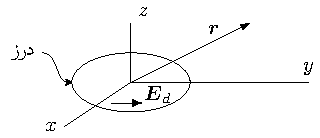
\includegraphics{emtAntennasAndRadiationApertureFourierTransform}
\caption{سطح \عددی{}z=0 پر درز میں برقی میدان \عددی{\kvec{E}_a} کو دور میدان فوریئر بدل ہے۔}
\label{شکل_اینٹینا_درز_فوریئر_بدل}
\end{figure}
فوریئر بدل کی یاد تازہ کرنے کے بعد اصل موضوع پر واپس آتے ہیں۔شکل \حوالہ{شکل_اینٹینا_درز_فوریئر_بدل} میں \عددی{z=0} سطح پر درز دکھایا گیا ہے جس پر برقی میدان
 \عددی{\kvec{E}_d} ہے۔یہ میدان \عددی{z<0} خطے میں موجود کثافت برقی رو کی وجہ سے پایا جاتا ہے۔ہمیں اس کثافت برقی رو کی ضرورت نہیں پڑے گی۔درز کا رقبہ \عددی{S_d} ہے۔آئیں درز پر موجود میدان سے خالی خلاء میں کہیں دور پیدا میدان دریافت کریں۔ 

میکس ویل کی مساوات \عددی{\nabla \times \kvec{E}=-\tfrac{\partial \kvec{B}}{\partial t}} کے گردش کو
\begin{align*}
\nabla \times \nabla \times \kvec{E}=\nabla \nabla \cdot \kvec{E}-\nabla^2 \kvec{E}&=-j \omega \mu_0 \nabla \times \kvec{H} \\
&=-j \omega \mu_0 (\kvec{J}+j \omega \epsilon_0 \kvec{E})
\end{align*}
لکھا جا سکتا ہے جہاں دوسری قدم پر \عددی{\nabla \times \kvec{H}=\kvec{J}+\tfrac{\partial \kvec{D}}{\partial t}} پر کیا گیا ہے۔ساتھ ہی ساتھ \عددی{\kvec{B}=\mu_0 \kvec{H}} اور \عددی{\kvec{D}=\epsilon_0 \kvec{E}} کے علاوہ \عددی{\tfrac{\partial \kvec{E}}{\partial t}=j \omega \kvec{E}} اور 
\عددی{\tfrac{\partial \kvec{H}}{\partial t}=j \omega \kvec{H}} کا بھی استعمال کیا گیا ہے۔ شکل \حوالہ{شکل_اینٹینا_درز_فوریئر_بدل} میں درز سے دور خالی خلاء میں نہ کوئی کثافت بار پائی جاتی ہے اور نہ ہی کثافت برقی رو۔یوں مندرجہ بالا مساوات میں دور مقام پر \عددی{\kvec{J}=0} اور  
\begin{align}\label{مساوات_اینٹینا_فوریئر_الف}
\nabla \cdot \kvec{E}&=0
\end{align}
پر کرتے ہوئے
\begin{align}\label{مساوات_اینٹینا_فوریئر_ب}
\nabla^2 \kvec{E}+k_0^2 \kvec{E}=0
\end{align}
حاصل ہوتا ہے جہاں
\begin{align}
k_0= \omega \sqrt{ \mu_0 \epsilon_0}
\end{align}
لکھا گیا ہے۔مساوات \حوالہ{مساوات_اینٹینا_فوریئر_الف} اور مساوات \حوالہ{مساوات_اینٹینا_فوریئر_ب} کو کارتیسی محدد میں یوں لکھا جائے گا۔
\begin{align}
\frac{\partial E_x(x,y,z)}{\partial x}+\frac{\partial E_y(x,y,z)}{\partial y}+\frac{\partial E_z(x,y,z)}{\partial z}&=0 \label{مساوات_اینٹینا_فوریئر_پ}\\
\left(\frac{\partial^2}{\partial x^2}+\frac{\partial^2}{\partial y^2}+\frac{\partial^2}{\partial z^2} +k_0^2\right) \kvec{E}(x,y,z)&=0\label{مساوات_اینٹینا_فوریئر_ت}
\end{align}
ان دو مساوات کا فوریئر بدل مساوات \حوالہ{مساوات_اینٹینا_فوریئر_بدل_ث} کی مدد سے لکھتے ہیں
\begin{align}
k_x E_x(k_x,k_y,k_z)+k_y E_y(k_x,k_y,k_z)+j \frac{\partial E_z(k_x,k_y,k_z)}{\partial z}&=0\label{مساوات_اینٹینا_فوریئر_ٹ}\\
\left[\frac{\partial^2}{\partial z^2}+(k_0^2-k_x^2-k_y^2)\right] \kvec{E}(k_x,k_y,k_z)&=0\label{مساوات_اینٹینا_فوریئر_ث}
\end{align}
 جہاں \عددی{u(x,y,z)=E(x,y,z)} لیتے ہوئے \عددی{U(k_x,k_y,k_z)=E(k_x,k_y,k_z)} لکھا گیا ہے۔یہاں بہتر ہوتا کہ برقی میدان اور اس کے فوریئر بدل کے لئے میں علیحدہ علیحدہ علامات استعمال کرتا لیکن امید کی جاتی ہے کہ \عددی{E(x,y,z)} کے آزاد متغیرات \عددی{(x,y,z)} سے \عددی{E(x,y,z)} کو اصل تفاعل اور \عددی{E(k_x,k_y,k_z)} کے آزاد متغیرات \عددی{(k_x,k_y,k_z)} سے  \عددی{E(k_x,k_y,k_z)}  کو فوریئر بدل سمجھا جا سکتا ہے۔

مندرجہ بالا مساوات میں
\begin{align}\label{مساوات_اینٹینا_حرکی_مستقل_الف}
k_0^2-k_x^2-k_y^2=k_z^2
\end{align}
لکھتے ہوئے
\begin{align}
\frac{\partial^2 \kvec{E}(k_x,k_y,k_z)}{\partial z^2}+k_z^2\kvec{E}(k_x,k_y,k_z)&=0
\end{align}
حاصل ہوتا ہے جس کے حل \عددی{e^{\mp j k_z z}} صورت رکھتے ہیں۔ان میں \عددی{e^{-j k_z z}} کارتیسی نظام میں بڑھتے \عددی{z} جانب حرکت کرتی موج ہے جبکہ \عددی{e^{j k_z z}} گھٹتے  \عددی{z} جانب حرکت کرتی موج ہے۔ہم پہلے جواب کو تسلیم کرتے ہیں لہٰذا مندرجہ بالا مساوات کا حل
\begin{align}\label{مساوات_اینٹینا_فوریئر_ج}
\kvec{E}(k_x,k_y,k_z)=\kvec{f}(k_x,k_y) e^{-j k_z z}
\end{align}
لکھا جا سکتا ہے جہاں \عددی{\kvec{f}(k_x,k_y)} دریافت کرنا باقی ہے۔

مساوات \حوالہ{مساوات_اینٹینا_فوریئر_ج} کو مساوات \حوالہ{مساوات_اینٹینا_فوریئر_ٹ} میں پر کرنے سے
\begin{align}
k_x f_x+k_y f_y+k_z f_z=0
\end{align}
یعنی
\begin{align}\label{مساوات_اینٹینا_فوریئر_چ}
\kvec{k} \cdot \kvec{f}=0
\end{align}
ملتا ہے جہاں \عددی{\kvec{f}=f_x \ax+f_y \ay+f_z \az} اور \عددی{\kvec{k}=k_x \ax+k_y \ay+k_z \az} لکھے گئے ہیں۔مساوات \حوالہ{مساوات_اینٹینا_فوریئر_چ} کے تحت \عددی{f_x}، \عددی{f_y} اور \عددی{f_z} تینوں آزاد متغیرات نہیں ہو سکتے۔ان میں کوئی دو آزاد ہونے کی صورت میں تیسرے جزو کو ان دو اجزاء سے حاصل کیا جا سکتا ہے لہٰذا تیسرا جزو تابع متغیرہ ہو گا۔یہ حقیقت برقی میدان پر بھی لاگو ہوتی ہے  جہاں اس حقیقت کو \عددی{\nabla \cdot \kvec{E}=0} لکھا جاتا ہے۔

اصل برقی میدان \عددی{\kvec{E}(x,y,z)} حاصل کرنے کی خاطر \عددی{\kvec{E}(k_x,k_y,k_z)} کا الٹ فوریئر بدل لیتے ہیں
\begin{align*}
\kvec{E}(x,y,z)&=\frac{1}{4\pi^2} \int_{-\infty}^{\infty} \int_{-\infty}^{\infty} \kvec{E}(k_x,k_y,k_z) e^{-j k_x x -j k_y y} \dif k_x \dif k_y\\
&=\frac{1}{4\pi^2} \int_{-\infty}^{\infty} \int_{-\infty}^{\infty} \kvec{f}(k_x,k_y)e^{-j k_x x -j k_y y-j k_z z} \dif k_x \dif k_y
\end{align*}
 جہاں مساوات \حوالہ{مساوات_اینٹینا_فوریئر_ج} استعمال کیا گیا ہے۔کارتیسی محدد میں سمتی فاصلے  کو \عددی{\kvec{r}=x \ax+y \ay+z \az} لکھا جا سکتا ہے۔یوں 
\begin{align*}
k_x x+k_y y+k_z z=\kvec{k}\cdot\kvec{r}
\end{align*}
لکھتے ہوئے مندرجہ بالا مساوات کو
\begin{align}\label{مساوات_اینٹینا_دور_میدان_الف}
\kvec{E}(x,y,z)&=\frac{1}{4\pi^2} \int_{-\infty}^{\infty} \int_{-\infty}^{\infty} \kvec{f}(k_x,k_y)e^{-j \kvec{k} \cdot \kvec{r}} \dif k_x \dif k_y \quad \text{درز کا میدان}
\end{align}
لکھا جا سکتا ہے۔اس مساوات میں تکمل کے اندر \عددی{\kvec{f} e^{-j \kvec{k}\cdot \kvec{r}}} حرکت کرتی موج کو ظاہر کرتی ہے۔یوں \عددی{z>0} خطے میں میدان حرکت کرتی موج ہو گی۔ مساوات \حوالہ{مساوات_اینٹینا_حرکی_مستقل_الف} سے واضح ہے کہ \عددی{\abs{\kvec{k}}=k_0} کے برابر ہے۔یوں اگر \عددی{k_x^2+k_y^2>k_0^2} ہو تب \عددی{k_z} خیالی مقدار ہو گا۔ایسی صورت میں موج \عددی{z} سمت میں \عددی{e^{-k_z z}} کی رفتار سے  گھٹے گی جو فنا پذیر\فرہنگ{فنا پذیر}\فرہنگ{evanescent wave} موج کی نشانی ہے۔ یہ فنا پذیر موج درز کے سامنے قریبی میدان کو ظاہر  کرتی ہے۔اگر \عددی{k_x} اور \عددی{k_y} کو کارتیسی محدد پر دکھایا جائے تو جو قیمت \عددی{k_0} رداس کے دائرے سے باہر ہو، وہ فنا پذیر موج کو ظاہر کریں گے جبکہ اس دائرے کے اندر قیمتیں دور میدان کو ظاہر کرتی ہیں۔

مساوات \حوالہ{مساوات_اینٹینا_دور_میدان_الف} کے حاصل کردہ میدان کی قیمت سطح \عددی{z=0} پر  عین شکل \حوالہ{شکل_اینٹینا_درز_فوریئر_بدل} کے میدان برابر ہو گی۔اس شکل میں میدان \عددی{z=0} سطح کے متوازی ہے۔یوں اگر \عددی{\kvec{f}} کے \عددی{x} اور \عددی{y} اجزاء کو \عددی{\kvec{f}_m} سے ظاہر کیا جائے (یعنی \عددی{\kvec{f}_m=f_x \ax+f_y \ay}) تب
\begin{align}\label{مساوات_اینٹینا_دور_میدان_فوریئر_الف}
\kvec{E}_d (x,y)=\kvec{E}_m(x,y,0)=\frac{1}{4\pi^2} \int_{-\infty}^{\infty} \int_{-\infty}^{\infty} \kvec{f}_m(k_x,k_y)e^{-j k_x x -j k_y y} \dif k_x \dif k_y
\end{align}
ہو گا۔مساوات \حوالہ{مساوات_اینٹینا_دور_میدان_فوریئر_الف} فوریئر بدل کی مساوات ہے لہٰذا اس کا الٹ فوریئر بدل یوں
\begin{align}\label{مساوات_اینٹینا_دور_میدان_فوریئر_ب}
\kvec{f}_m(k_x,k_y)=\iint_{S_d} \kvec{E}_d(x,y) e^{j k_x x +j k_y y} \dif x \dif y
\end{align}
 لکھنا ممکن ہے۔اس مساوات کے تحت درز پر میدان کا فوریئر بدل دور میدان کو ظاہر کرتی ہے۔مساوات \حوالہ{مساوات_اینٹینا_فوریئر_چ} سے
\begin{align}\label{مساوات_اینٹینا_دور_میدان_فوریئر_پ}
f_z=\frac{-\kvec{k}_m\cdot\kvec{f}_m}{k_z}=\frac{-k_x f_x-k_y f_y}{\sqrt{k_0^2-k_x^2-k_y^2}}
\end{align}
لکھا جا سکتا ہے۔مندرجہ بالا دو مساوات مل کر  \عددی{\kvec{f}} کے تینوں اجزاء دیتے ہیں۔

مساوات \حوالہ{مساوات_اینٹینا_دور_میدان_فوریئر_ب} اور مساوات \حوالہ{مساوات_اینٹینا_دور_میدان_فوریئر_ب} سے حاصل \عددی{\kvec{f}(k_x,k_y)}  کو مساوات \حوالہ{مساوات_اینٹینا_دور_میدان_الف} میں پر کرتے ہوئے درز کا میدان حاصل کیا جاتا ہے۔آئیں اب مساوات \حوالہ{مساوات_اینٹینا_دور_میدان_الف} کا حل حاصل کریں۔

ہمیں دور میدان سے غرض ہے۔اس حقیقت کو استعمال کرتے ہوئے ہم  مساوات \حوالہ{مساوات_اینٹینا_دور_میدان_الف} کو صرف دور میدان کے لئے حل کرتے ہیں۔ایسا کرنے کی خاطر جو ترکیب بروئے کار لائی جائے گی اس کی بنیاد اس حقیقت پر ہے کہ \عددی{r} کی قیمت زیادہ ہونے کی صورت میں  \عددی{e^{-j \kvec{k}\cdot \kvec{r}}} نہایت تیزی سے ارتعاش کرتا تفاعل ہو گا۔یوں مساوات \حوالہ{مساوات_اینٹینا_دور_میدان_الف} میں \عددی{k_x k_y} سطح کے مختلف نقطوں پر اس تفاعل کی قیمتیں ایک دونوں کو ختم کریں گی۔اس تفاعل میں \عددی{r} کی قیمت زیادہ ہونے کی وجہ سے  \عددی{k_x k_y} سطح پر قریب ترین  نقطوں کے درمیان بھی اتنا زاویائی فرق \عددی{j \kvec{k}\cdot \kvec{r}} پایا جاتا ہے کہ تکمل میں ان کا مجموعہ قابل نظر انداز ہوتا ہے۔البتہ ایسے مقام جہاں زاویائی فرق نہ پایا جاتا ہو،  دور میدان میں کردار ادا کرتے ہیں۔ان مقام جنہیں \اصطلاح{ساکن نقطے}\فرہنگ{ساکن نقطے}\حاشیہب{stationary points}\فرہنگ{stationary points} کہا جاتا ہے کو مندرجہ ذیل مساوات سے حاصل کیا جاتا ہے۔
\begin{gather}
  \begin{aligned}\label{مساوات_اینٹینا_ساکن_نقطے}
\frac{\partial (\kvec{k}\cdot \kvec{r})}{\partial k_x}&=0\\
\frac{\partial (\kvec{k}\cdot \kvec{r})}{\partial k_y}&=0
\end{aligned}
\end{gather}
ساکن نقطوں پر \عددی{e^{-j \kvec{k}\cdot\kvec{r}}} کی قیمت میں ٹھراو پایا جاتا ہے لہٰذا تکمل میں ایسے مقام کا مجموعہ دور میدان میں کردار ادا کرتا ہے۔ساکن مقام \عددی{k_1 k_2} سطح پر چھوٹا خطہ ہو گا۔اس چھوٹے خطے  میں \عددی{\kvec{f}(k_x,k_y)} کے قیمت میں تبدیلی کو رد کرتے ہوئے اسے اٹل تصور کیا جاتا ہے۔اس طرح  \عددی{\kvec{f}(k_x,k_y)} کو تکمل کے باہر منتقل کیا جاتا ہے۔بقایا تکمل میں صرف \عددی{e^{-j \kvec{k}\cdot \kvec{r}}} رہ جاتا ہے جسے حاصل کرنا ممکن ہے۔

اگر \عددی{\kvec{k}\cdot \kvec{r}=k_x x+k_y y +k_z z} میں کروی محدد کے متغیرات استعمال کرتے ہوئے \عددی{{x=r\sin \theta \cos \phi}}، \عددی{{y=r\sin\theta\sin\phi}} اور \عددی{{z=r\cos\theta}} پر کئے جائیں تو
\begin{align}
\kvec{k}\cdot\kvec{r}=r(k_x \sin\theta\cos\phi+k_y\sin\theta\sin\phi+\sqrt{k_0^2-k_x^2-k_y^2}\cos \theta)
\end{align}
حاصل ہوتا ہے۔ مساوات \حوالہ{مساوات_اینٹینا_ساکن_نقطے} استعمال کرتے ہوئے ساکن نقطہ
\begin{align}
k_x&=k_1=k_0 \sin\theta\cos\phi\\
k_y&=k_2=k_0\sin\theta\sin\phi
\end{align}
حاصل ہوتا ہے۔ساکن نقطے کے قریب \اصطلاح{ٹیلر تسلسل}\فرہنگ{ٹیلر تسلسل}\فرہنگ{تسلسل!ٹیلر}\حاشیہب{Taylor series}\فرہنگ{Taylor series} کے استعمال سے ہم لکھ سکتے ہیں
\begin{align*}
\kvec{k}\cdot\kvec{r}&=k_0 r +\frac{1}{2}\frac{\partial^2 \kvec{k}\cdot\kvec{r}  }{\partial k_x^2} (k_x-k_1)^2+\frac{1}{2}\frac{\partial^2 \kvec{k}\cdot\kvec{r}  }{\partial k_y^2} (k_y-k_2)^2+\frac{\partial^2 \kvec{k}\cdot\kvec{r}  }{\partial k_x \partial k_y} (k_x-k_1)(k_y-k_2)\\
&=k_0 r-(A u^2+B v^2+C u v)
\end{align*}
جہاں \عددی{u=k_x-k_1}، \عددی{v=k_y-k_2} ہیں جبکہ
\begin{gather}
\begin{aligned}\label{مساوات_اینٹینا_ساکن_نقطہ_مستقل}
A&=\frac{r}{2}\left(\frac{1}{k_0}+\frac{k_1^2}{k_0^3 \cos^2 \theta}\right)\\
B&=\frac{r}{2}\left(\frac{1}{k_0}+\frac{k_2^2}{k_0^3 \cos^2 \theta}\right)\\
C&=\frac{k_1 k_2 r}{k_0^3 \cos^2 \theta}
\end{aligned}
\end{gather}
ہیں۔چونکہ \عددی{\tfrac{\partial}{\partial k_x}=0} اور \عددی{\tfrac{\partial}{\partial k_y}=0} ہیں لہٰذا  انہیں بالا ٹیلر تسلسل میں شامل نہیں کیا گیا۔

ان حقائق کو استعمال کرتے ہوئے مساوات \حوالہ{مساوات_اینٹینا_دور_میدان_الف} کو مندرجہ ذیل صورت میں لکھنا ممکن ہے
\begin{align}
\kvec{E}(\kvec{r}) \approx \frac{e^{-jk_0 r}}{4\pi^2}\kvec{f}(k_0 \sin \theta \cos \phi,k_0 \sin\theta\sin\phi)\iint \limits_{\Delta s} e^{j (A u^2+ B v^2+C uv)} \dif u \dif v
\end{align}
جہاں تکمل  ساکن نقطے پر چھوٹی سطح \عددی{\Delta s} پر حاصل کیا جاتا ہے اور جہاں \عددی{\kvec{f}} کی قیمت اٹل تصور کرتے ہوئے ساکن نقطے پر \عددی{\kvec{f}} کی قیمت لی گئی ہے۔یہاں ایک مرتبہ دوبارہ اس حقیقت کو سامنے رکھتے ہوئے آگے بڑھتے ہیں کہ چونکہ \عددی{A}، \عددی{B} اور \عددی{C} کی قیمتیں \عددی{r} کے مماثل ہیں لہٰذا یہ قیمتیں بھی بہت بڑی ہوں گی۔ یوں \عددی{u} اور \عددی{v} کے تبدیلی سے مندرجہ بالا تکمل میں \عددی{A}، \عددی{B} اور \عددی{C} پر منحصر تفاعل بھی تیزی سے ارتعاش کرے گی جس کی وجہ سے مختلف نقطوں پر تفاعل آپس میں جمع نہ ہو پائے گا۔اس حقیقت کی بنا پر اگر تکمل کو لامحدود سطح پر لیا جائے تو حاصل جواب پر کوئی اثر نہیں پڑنا چاہیے۔ایسا ہی کرتے ہوئے مندرجہ بالا مساوات میں
\begin{align}
\iint \limits_{-\infty}^{\infty} e^{j (A u^2+ B v^2+C uv)} \dif u \dif v
\end{align}
کا حل حاصل کرتے ہیں۔ہم
\begin{align*}
A u^2+Bv^2+Cuv=\left(\sqrt{A} u +\frac{C v}{2\sqrt{A}} \right)^2-\frac{C^2 v^2}{4A}+Bv^2
\end{align*}
لکھ کر \عددی{\sqrt{A} u +\tfrac{C v}{2\sqrt{A}}=w} پر کرتے ہوئے
\begin{align}
\iint \limits_{-\infty}^{\infty} e^{j w^2}e^{\frac{j(4AB-C^2)v^2}{4A}} \frac{\dif w}{\sqrt{A}} \dif v
\end{align}
لکھ سکتے ہیں۔ہم یہاں پہلے سے معلوم تکمل
\begin{align}
\int\limits_{-\infty}^{\infty}e^{j \gamma(x-x_0)^2} \dif x=\sqrt{\frac{\pi}{\gamma}} e^{j \frac{\pi}{4}}
\end{align}
کا استعمال کرتے ہوئے
 \begin{align*}
\iint \limits_{-\infty}^{\infty} e^{j w^2}e^{\frac{j(4AB-C^2)v^2}{4A}} \frac{\dif w}{\sqrt{A}} \dif v&=\frac{j 2\pi}{\sqrt{4AB-C^2}}\\
&=j 2\pi \frac{k_0}{r}\cos \theta
\end{align*}
حاصل کرتے ہیں۔مساوات \حوالہ{مساوات_اینٹینا_ساکن_نقطہ_مستقل} میں دئے مستقل پر کرتے ہوئے یوں مساوات \حوالہ{مساوات_اینٹینا_دور_میدان_الف} کا حل 
\begin{align}\label{مساوات_اینٹینا_فوریئر_بدل}
\kvec{E}(\kvec{r})\approx \frac{j k_0 \cos \theta}{2\pi r} e^{-j k_0 r}\kvec{f}(k_0 \sin \theta \cos \phi,k_0 \sin\theta \sin\phi)
\end{align}
حاصل ہوتا ہے جہاں
\begin{align}
\kvec{f}_m(k_x,k_y)=\iint\limits_{S_a} \kvec{E}_d(x,y) e^{j k_x x +j k_y y} \dif x \dif y
\end{align}
کے برابر ہے۔

مساوات \حوالہ{مساوات_اینٹینا_فوریئر_بدل} کہتی ہے دور میدان، درز پر میدان کا فوریئر بدل ہے جہاں فوریئر بدل میں \عددی{k_x} کی جگہ \عددی{k_0\sin\theta\cos\phi} اور \عددی{k_y} کی جگہ \عددی{k_0\sin\theta\sin\phi} پر کیا جاتا ہے۔

چونکہ \عددی{\kvec{k}\cdot\kvec{f}=0} کے برابر ہے لہٰذا \عددی{\kvec{k}} کی سمت میں \عددی{\kvec{f}} کی قیمت صفر کے برابر ہے یعنی \عددی{z} محدد پر صرف \عددی{f_x} اور \عددی{f_x} پایا جائے گا۔کروی محدد میں یوں
\begin{align}\label{مساوات_اینٹینا_دور_میدان_بذریعہ_فوریئر_بدل}
\kvec{E}(\kvec{r})=j k_0 \frac{e^{-j k_0 r}}{2\pi r}\left[\atheta (f_x \cos\phi+f_y \sin\phi)+\aphi \cos \theta (f_y\cos\phi-f_x\sin\phi) \right]
\end{align}
لکھا جا سکتا ہے۔مقناطیسی میدان \عددی{\tfrac{\kvec{E}}{\kvec{H}}=Z_0} سے حاصل کیا جا سکتا ہے۔
%===================
\ابتدا{مثال}
مستطیل درز کی \عددی{x} سمت میں لمبائی \عددی{2a} ہے جبکہ \عددی{y} سمت میں اس کی لمبائی \عددی{2b} ہے۔درز \عددی{z=0} پر پایا جاتا  ہے جبکہ اس پر
 میدان \عددی{\kvec{E}_d=E_0\ax} ہے۔دور میدان حاصل کریں۔

حل:پہلے \عددی{\kvec{f}_m} حاصل کرتے ہیں۔
\begin{align*}
\kvec{f}_m&=E_0 \ax \int_{-a}^{a}\int_{-b}^{b} e^{j k_x x +j k_y y} \dif x \dif y\\
&=4 a b E_0 \ax \frac{\sin k_x a}{k_x a}\frac{\sin k_y b}{k_y b}\\
&=4 a b E_0 \ax \frac{\sin k_0 a \sin \theta \cos \phi}{k_0 a\sin \theta \cos \phi}\frac{\sin k_0 b \sin \theta \sin\phi}{k_0 b\sin\theta\sin\phi}\\
&=4 a b E_0 \ax \frac{\sin u}{u} \frac{\sin v}{v}
\end{align*}
اب دور میدان مساوات \حوالہ{مساوات_اینٹینا_دور_میدان_بذریعہ_فوریئر_بدل} سے لکھتے ہیں۔
\begin{align*}
\kvec{E}(\kvec{r})=\frac{j k_0 4 a bE_0}{2\pi r}e^{-j k_0 r}\frac{\sin u}{u}\frac{\sin v}{v} (\atheta \cos\phi-\aphi \sin\phi\cos\theta)
\end{align*}
\انتہا{مثال}
%====================================
%==================================================
\حصہ{خطی اینٹینا}
مختصر جفت قطب ہم دیکھ چکے ہیں جہاں جفت قطب کی لمبائی طول موج سے بہت کم \عددیء{l \ll \lambda} تھی۔متعدد تعداد کے نقطہ منبع کو سیدھ میں قریب قریب رکھنے سے کسی بھی لمبائی کا اینٹینا حاصل کیا جا سکتا ہے۔آئیں ایسی لمبی اینٹینا پر غور کریں۔اینٹینا پر سائن نما برقی رو تصور کی جائے گی۔

\begin{figure}
\centering
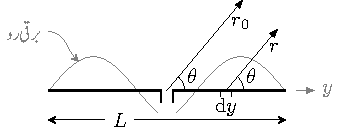
\includegraphics{emtAntennasLinearCentreFedWithSinusoidalCurrent}
\caption{خطی اینٹینا پر سائن نما برقی رو پائی جاتی ہے۔}
\label{شکل_اینٹینا_خطی_سائن_نما_برقی_رو}
\end{figure}

شکل \حوالہ{شکل_اینٹینا_خطی_سائن_نما_برقی_رو} میں \عددیء{L} لمبائی کا اینٹینا دکھایا گیا ہے جسے بالکل درمیان سے برقی رو مہیا کی گئی ہے۔اینٹینا کے دونوں بالکل یکساں نصف اطراف میں برقی رو بھی ہم شکل ہے۔ہم \عددیء{L} کے چھوٹے چھوٹے ٹکڑوں \عددیء{\dif y} کو انفرادی جفت قطب تصور کرتے ہوئے ان سب کے میدان کا مجموعہ حاصل کرتے ہوئے اس اینٹینا کا دور میدان حاصل کریں گے۔

تجربے سے ثابت ہوتا ہے کہ ایسی اینٹینا میں برقی رو
\begin{align}\label{مساوات_اینٹینا_لمبا_اینٹینا_برقی_رو}
I=
\begin{dcases}
I_0 \sin \left[\frac{2\pi}{\lambda} \left(\frac{L}{2} + y \right) \right] & \quad y<0\\ 
I_0 \sin \left[\frac{2\pi}{\lambda} \left(\frac{L}{2} - y \right) \right] & \quad y>0
\end{dcases}
\end{align}
صورت رکھتی ہے۔مختصر جفت قطب کی لمبائی کو \عددیء{\dif y} اور اس کے دور میدان کو \عددیء{\dif E_{\theta}} لکھتے ہوئے  مساوات \حوالہ{مساوات_اینٹینا_جفت_قطب_دور_میدان}
\begin{align}
\dif E_{\theta}&=j \frac{30 I \beta \dif y}{r} \sin \theta e^{j(\omega t-\beta r)}
\end{align}
یعنی
\begin{align}
\dif E_{\theta}&=\frac{j 60 \pi    e^{j(\omega t-\beta r_0)}}{r_0 \lambda}\sin \theta  I e^{j\beta y \cos \theta} \dif y
\end{align}
دیتی ہے۔یوں \عددیء{L} لمبے اینٹینا کا میدان
\begin{align}
E_{\theta}&=k \sin \theta \int \limits_{-L/2}^{L/2} I e^{j\beta y \cos \theta} \dif y
\end{align}
ہو گا جہاں
\begin{align}
k=\frac{j 60 \pi  e^{j(\omega t-\beta r_0)}}{r_0 \lambda} 
\end{align}
لکھا گیا ہے۔مساوات \حوالہ{مساوات_اینٹینا_لمبا_اینٹینا_برقی_رو} استعمال کرتے اور تکمل لیتے ہوئے
\begin{align}\label{مساوات_اینٹینا_دور_میدان_خطی_اینٹینا_عمومی}
E_{\theta}=\frac{j 60 [I_0]}{r_0} \left \{ \frac{\cos[(\beta L \cos \theta)/2]-\cos(\beta L/2)}{\sin \theta} \right \} \quad \text{\RL{خطی اینٹینا کی عمومی مساوات}}
\end{align}
حاصل ہوتا ہے جہاں \عددیء{[I_0]=I_0 e^{j (\omega t-\beta r_0)}} تاخیری برقی رو ہے۔\عددیء{\tfrac{\lambda}{2}} جفت قطب کی صورت میں اسے
\begin{align}\label{مساوات_اینٹینا_نصف_جفت_قطب_الف}
E_{\theta}=\frac{j 60 [I_0]}{r_0}\frac{\cos [\frac{\pi}{2} \cos \theta]}{\sin \theta} \quad \text{\RL{$\tfrac{\lambda}{2}$ جفت قطب}}
\end{align}
لکھا جا سکتا ہے۔

میدان کی شکل مساوات \حوالہ{مساوات_اینٹینا_دور_میدان_خطی_اینٹینا_عمومی} کے دائیں جانب قوسین میں بند جزو پر منحصر ہے جسے \عددیء{\tfrac{\lambda}{2}} جفت قطب کی صورت میں
\begin{align}\label{مساوات_اینٹینا_نصف_طول_موج_اینٹینا}
E_{\theta} =\frac{\cos [\frac{\pi}{2} \cos \theta]}{\sin \theta} \quad \quad \text{\RL{$\frac{\lambda}{2}$ جفت قطب}}
\end{align}
اور \عددیء{1.5 \lambda} جفت قطب کی صورت میں
\begin{align}
E_{\theta} =\frac{\cos [\frac{3\pi}{2} \cos \theta]}{\sin \theta} \quad \quad \text{\RL{$\frac{3\lambda}{2}$ جفت قطب}}
\end{align}
لکھا جا سکتا ہے۔

شکل \حوالہ{شکل_اینٹینا_نصف_جفت_قطب_برقی_رو} میں \عددیء{\tfrac{\lambda}{2}} اور \عددیء{\tfrac{3\lambda}{2}} جفت قطب اور ان کے شعاع نلکی محدد پر دکھائے گئے ہیں۔جفت قطب پر برقی رو کی سمتیں تیر کی نشان سے دکھائے گئے ہیں۔

\begin{figure}
\centering
\begin{subfigure}{0.4\textwidth}
\centering
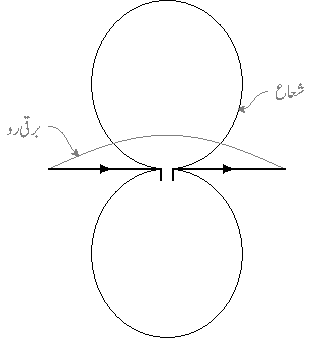
\includegraphics{emtAntennasAndRadiationHalfDipoleCurrentAndField}
\caption*{الف: $\frac{\lambda}{2}$ جفت قطب}
\end{subfigure}%
%
\begin{subfigure}{0.4\textwidth}
\centering
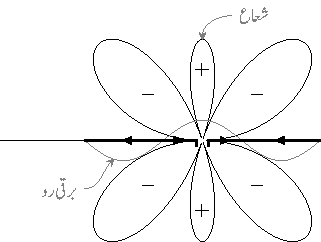
\includegraphics{emtAntennasAndRadiationOneAndHalfDipoleCurrentAndField}
\caption*{ب: $\frac{3\lambda}{2}$ جفت قطب}
\end{subfigure}%
\caption{$0.5\lambda$ اور $1.5\lambda$ جفت قطب کے دور میدان۔}
\label{شکل_اینٹینا_نصف_جفت_قطب_برقی_رو}
\end{figure}%

شکل-ب میں میدان کے شعاعوں میں \عددیء{180^{\circ}} کا زاویائی فرق پایا جاتا ہے۔

جفت قطب کو محور لیتے ہوئے دئے گئے نقش کو اس کے گرد گمانے سے تین رُخی نقش حاصل ہو گا۔ 

اوسط پوئنٹنگ سمتیہ کا بڑی رداس کے کرہ پر سطحی تکمل
\begin{align}
P=\int \limits_{0}^{2\pi}\int \limits_{0}^{\pi}  \frac{\abs{E_{\theta}}^2}{2 Z} r^2 \sin \theta \dif \theta \dif \phi
\end{align}
عددی طریقے سے حاصل کرتے ہوئے کل اخراجی مزاحمت  \عددیء{R} حاصل کی جاتی ہے۔اس مساوات میں \عددیء{\abs{E_{\theta}}} کو مساوات \حوالہ{مساوات_اینٹینا_نصف_جفت_قطب_الف} سے پر کرتے ہوئے 
\begin{align*}
P&= \frac{15 I_0^2}{\pi}\int \limits_{0}^{2\pi}\int \limits_{0}^{\pi}  \frac{\cos^2 [\frac{\pi}{2} \cos \theta]}{\sin \theta} \dif \theta \dif \phi
\end{align*}
حاصل ہوتا ہے جہاں \عددیء{Z_0=120\pi} اور \عددیء{r=r_0} لکھے گئے ہیں۔بیرونی تکمل پہلے لیتے ہوئے
\begin{align}\label{مساوات_اینٹینا_نصف_طول_موج_اخراجی_طاقت_الف}
P&= 30 I_0^2\int \limits_{0}^{\pi}  \frac{\cos^2 [\frac{\pi}{2} \cos \theta]}{\sin \theta} \dif \theta
\end{align}
ملتا ہے۔اس مساوات کو عددی طریقے سے حل کرتے ہیں۔ایسا کرنے کی خاطر اسے مجموعے
\begin{align}
P=\sum_{i=0}^{n} 30 I_0^2  \frac{\cos^2 [\frac{\pi}{2} \cos \theta]}{\sin \theta} \Delta  \theta =\sum_{i=0}^{n} p(\theta) \Delta \theta
\end{align}
کی شکل میں لکھتے ہیں جہاں
\begin{align}\label{مساوات_اینٹینا_اخراجی_مزاحمت_عددی_الف}
p(\theta)=30 I_0^2  \frac{\cos^2 [\frac{\pi}{2} \cos \theta]}{\sin \theta}
\end{align}
لکھا گیا ہے۔ شکل \حوالہ{شکل_اینٹینا_اخراجی_مزاحمت_عددی_حل} میں کارتیسی محدد پر  تفاعل \عددیء{p(\theta)}  کو دکھایا گیا ہے۔افقی محدد پر \عددیء{\theta=0} تا \عددیء{\theta=\pi} ہے  جبکہ عمودی محدد پر \عددیء{p(\theta)} ہے۔اگر \عددیء{\theta=0} تا \عددیء{\pi} کو \عددیء{n} برابر ٹکڑوں میں تقسیم کیا جائے تو ہر ٹکڑے کی چوڑائی \عددیء{\tfrac{\pi}{n}} ہو گی۔گراف کے ایسے ہر ٹکڑے کو مستطیل تصور کیا جا سکتا ہے۔ان تمام مستطیل کے رقبے جمع کرتے ہوئے تکمل حاصل کیا جاتا ہے۔اسے کہتے ہیں عددی طریقہ۔
\begin{figure}
\centering
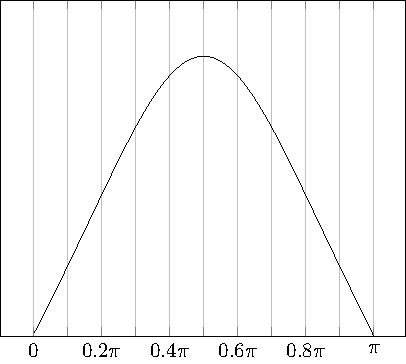
\includegraphics{emtAntennasAndRadiationHalfDipoleResistanceNumericalSolution}
\caption{اخراجی مزاحمت کا عددی حل۔}
\label{شکل_اینٹینا_اخراجی_مزاحمت_عددی_حل}
\end{figure}

شکل میں \عددیء{n=10} لیا گیا ہے۔یوں ہمیں دس مستطیل کے رقبے حاصل کرنے ہیں۔ہر مستطیل کے دونوں اطراف کے قد کی اوسط قیمت کو مستطیل کا قد تصور کیا جائے گا۔بائیں بازو سے شروع کرتے ہوئے پہلے مستطیل کے بائیں طرف کا قد \عددیء{0} ہے جبکہ اس کے دائیں طرف کا قد \عددیء{\theta=0.1\pi} پر مساوات  \حوالہ{مساوات_اینٹینا_اخراجی_مزاحمت_عددی_الف} سے
\begin{align}
p_1(\theta)=30 I_0^2  \frac{\cos^2 [\frac{\pi}{2} \cos (0.1\pi)]}{\sin (0.1\pi)}=\num{0.573} I_0^2
\end{align}
حاصل ہوتا ہے۔اسی طرح بقایا تمام نقطوں پر بھی قد حاصل کرتے ہوئے جدول \حوالہ{جدول_اینٹینا_عددی_اخراجی_مزاحمت} میں دیے گیے ہیں۔
\begin{table}
\caption{برابر زاویائی فاصلوں پر تفاعل کے قیمت۔}
\centering
\begin{tabular}{l l}
$\theta$ & $30 I_0^2 \, \frac{\cos^2 [\pi/2 \cos \theta]}{\sin \theta}$\\ [2pt]
\hline
$0.0 \pi$ & $0$\\ [0.5pt]
$0.1 \pi$ & $ 00.573 I_0^2$\\ [1pt]
$0.2 \pi$ & $04.457 I_0^2$\\ [1pt]
$0.3 \pi$ & $13.492 I_0^2$\\ [1pt]
$0.4 \pi$ & $24.677 I_0^2$\\[1pt]
$0.5 \pi$ & $30 I_0^2$\\ [1pt]
$0.6 \pi$ & $24.677 I_0^2 $\\ [1pt]
$0.7 \pi$ & $13.492 I_0^2$ \\ [1pt]
$0.8 \pi$ & $04.457 I_0^2$\\ [1pt]
$0.9 \pi$ & $00.573 I_0^2$\\ [1pt]
$1.0 \pi$ & $0$
\end{tabular}
\label{جدول_اینٹینا_عددی_اخراجی_مزاحمت}
\end{table}

شکل \حوالہ{شکل_اینٹینا_اخراجی_مزاحمت_عددی_حل} میں بائیں سے دوسرے مستطیل (\عددیء{\theta=0.1\pi} تا \عددیء{\theta=0.2\pi}) کا رقبہ
\begin{align*}
\text{رقبہ}&= \text{چوڑائی} \times \text{\RL{اوسط قد}} \\
&=0.1 \pi \times \left(\frac{0.573 I_0^2+4.457 I_0^2}{2} \right)\\
&=0.79 I_0^2
\end{align*}
ہے۔

جدول \حوالہ{جدول_اینٹینا_عددی_اخراجی_مزاحمت} کی مدد سے کل رقبہ
\begin{multline*}
P=0.1 \pi I_0^2 \left(\frac{0}{2}+0.573+4.457+13.492+24.677+30 \right.\\
\left. +24.677++13.492+4.457+0.573+\frac{0}{2}\right)
\end{multline*}
یعنی
\begin{align}\label{مساوات_اینٹینا_نصف_طول_موج_اخراجی_طاقت_ب}
P=36.5675 I_0^2
\end{align}
حاصل ہوتا ہے۔سائن نما برقی رو کی چوٹی \عددیء{I_0} ہونے کی صورت میں مزاحمت \عددیء{R} میں طاقت کا ضیاع \عددیء{\tfrac{1}{2}I^2_0 R} ہوتا ہے لہٰذا ان دونوں کو برابر لکھتے ہوئے
\begin{align*}
\frac{1}{2}I_0^2 R_{\text{اخراجی}} = 36.5675 I_0^2
\end{align*}
 \عددیء{\tfrac{\lambda}{2}} لمبائی کے جفت قطب کا اخراجی مزاحمت
\begin{align}
R_{\text{اخراجی}}=\SI{73.13}{\ohm} \quad \quad \text{\RL{$\frac{\lambda}{2}$ جفت قطب}}
\end{align}
حاصل ہوتا ہے۔ یہ وہ مزاحمت ہے جو اینٹینا کو طاقت مہیا کرنے یا اس سے طاقت وصول کرنے  والے ترسیلی تار کو نظر آتی ہے۔\عددیء{\tfrac{\lambda}{2}} اینٹینا کے اخراجی مزاحمت کا موازنہ مختصر جفت قطب کی اخراجی مزاحمت \عددیء{(\SI{0.63}{\ohm})} کے ساتھ کریں جسے  صفحہ \حوالہصفحہ{مثال_اینٹینا_کھمبا_اینٹینا} پر مثال \حوالہ{مثال_اینٹینا_کھمبا_اینٹینا} میں   حاصل کیا گیا ہے۔

اینٹینا کی رکاوٹ میں \عددیء{j 42.5} اوہم کا خیالی جزو \عددیء{(Z=73.1+j42.5)}\شناخت{صفحہ_اینٹینا_جفت_قطب_رکاوٹ} بھی پایا جاتا ہے۔اینٹینا کی لمبائی چند فی صد کم کرنے سے خیالی جزو صفر کیا جا سکتا ہے، البتہ اس سے حقیقی جزو قدر کم ہو کر \عددیء{\SI{70}{\ohm}} رہ جاتا ہے۔زیادہ سے زیادہ طاقت کی منتقلی کے لئے ضروری ہے کہ ایسے  اینٹینا کو \عددیء{\SI{70}{\ohm}}  قدرتی رکاوٹ کے ترسیلی تار کے ساتھ جوڑا جائے۔\عددیء{\tfrac{3\lambda}{2}} اینٹینا کا اخراجی مزاحمت \عددیء{\SI{100}{\ohm}} حاصل ہوتا ہے۔


%=====================
\ابتدا{مثال}
\عددیء{\tfrac{\lambda}{2}} لمبائی کے خطی اینٹینا کی سمتیت حاصل کریں۔

حل:مساوات \حوالہ{مساوات_اینٹینا_سمتیت_کی_ایک_اور_مساوات} میں مساوات \حوالہ{مساوات_اینٹینا_نصف_طول_موج_اینٹینا} پر کرتے ہوئے 
\begin{align}
D=\frac{4\pi}{\iint \limits_{4\pi} P_n(\theta,\phi) \dif \Omega}=\frac{4\pi}{2\pi \int_{0}^{\pi} \frac{\cos^2[\frac{\pi}{2}\cos \theta]}{\sin^2 \theta}\sin \theta \dif \theta}
\end{align}
حاصل ہوتا ہے۔اس کا مساوات\حوالہ{مساوات_اینٹینا_نصف_طول_موج_اخراجی_طاقت_الف} سے موازنہ کرتے ہوئے،  مساوات \حوالہ{مساوات_اینٹینا_نصف_طول_موج_اخراجی_طاقت_ب} میں حاصل کی گئی قیمت \عددیء{36.5675 I_0^2} استعمال کرتے ہوئے
\begin{align}
D=\frac{4\pi}{2\pi \left(\frac{36.5675 I_0^2}{30 I_0^2}\right)}=1.64
\end{align}
حاصل ہوتا ہے۔
\انتہا{مثال}
%===============


\حصہ{چلتی موج اینٹینا}
گزشتہ حصے میں خطی اینٹینا پر سائن نما برقی رو تصور کیا گیا۔ایسی دبلی موصل تار، جس کا قطر \عددیء{d} طول موج \عددیء{\lambda} سے بہت کم ہو \عددیء{d < \tfrac{\lambda}{100}} اور جس کا آخری سرا کھلے سرے ہو، کے برقی رو کی شکل تقریباً ایسی ہی ہوتی ہے۔

کئی طول موج لمبی خطی اینٹینا موصل زمین کے متوازی \عددیء{h} اونچائی پر پائی جاتی ہے۔ جیسے شکل \حوالہ{شکل_اینٹینا_موصل_سطح_خطی_اینٹینا_رو}-الف میں دکھایا گیا ہے، اس کو بائیں جانب سے ٹرانسمٹر\حاشیہب{transmitter} طاقت مہیا کرتا ہے۔خطی اینٹینا اور موصل زمین مل کر کھلے سرے ترسیلی تار کا کردار ادا کرتے ہیں۔یوں کھلے سر پر آمدی برقی رو اور یہاں سے انعکاسی برقی رو مل کر ساکن موج کو جنم دیتے ہیں جسے شکل-الف میں دکھایا گیا ہے۔تار کے کھلے سر پر برقی رو کے ساکن موج کا صفر پایا جاتا ہے جبکہ  \عددیء{\tfrac{\lambda}{4}} فاصلے پر اس کی چوٹی پائی جاتی ہے۔یہی برقی رو گزشتہ حصے میں خطی اینٹینا پر فرض کی گئی تھی۔

\begin{figure}
\centering
\begin{subfigure}{0.4\textwidth}
\centering
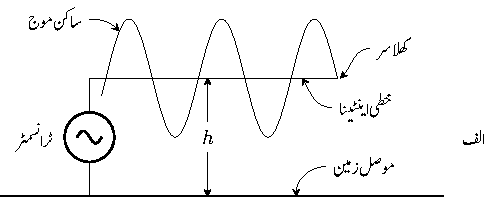
\includegraphics{emtAntennasAndRadiationCurrentOnLinearAntenna}
\end{subfigure}
\par\bigskip
\begin{subfigure}{0.4\textwidth}
\centering
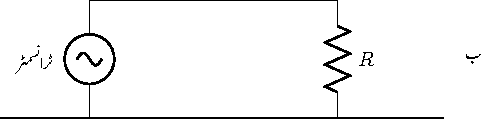
\includegraphics{emtAntennasAndRadiationTerminatedAntenna}
\end{subfigure}
\par\bigskip
\begin{subfigure}{0.4\textwidth}
\centering
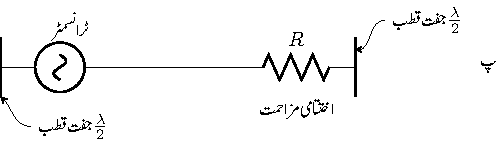
\includegraphics{emtAntennasAndRadiationTerminatedAntennaFarAwayFromGround}
\end{subfigure}
\caption{مسلسل موج اینٹینا۔}
\label{شکل_اینٹینا_موصل_سطح_خطی_اینٹینا_رو}
\end{figure}

آئیں اب ترسیلی تار کے قدرتی رکاوٹ کے برابر مزاحمت \عددیء{R}،  تار کے کھلے سر اور زمین کے درمیان جوڑیں۔ایسا کرنے کے بعد اینٹینا پر انعکاسی موج پیدا نہیں ہو گی۔تار میں قابل نظرانداز ضیاع کی صورت میں پوری لمبائی پر برقی رو کی قیمت یکساں ہو گی جبکہ لمبائی جانب بڑھتا زاویائی فرق پایا جائے گا۔اس طرح قدرتی رکاوٹ کے برابر مزاحمت سے اختتام کردہ اینٹینا کو شکل \حوالہ{شکل_اینٹینا_موصل_سطح_خطی_اینٹینا_رو}-ب میں دکھایا گیا ہے۔زمین سے دور خطی اینٹینا پر ایسی ہی مسلسل موج پیدا کرنے کی ترکیب شکل \حوالہ{شکل_اینٹینا_موصل_سطح_خطی_اینٹینا_رو}-پ میں دکھائی گئی ہے جہاں \عددیء{\tfrac{\lambda}{2}} اینٹینا کے وسطی نقطے کو زمین تصور کیا گیا ہے۔

مسلسل موج کے اس خطی اینٹینا کو چھوٹے چھوٹے، سلسلہ وار جڑے، لمبائی جانب اخراجی جفت قطب کا مجموعہ تصور کیا جا سکتا ہے۔ایسا شکل میں دکھایا گیا ہے۔مساوات \حوالہ{مساوات_اینٹینا_یکساں_قطار_تقابل_پذیر_میدان} غیر سمتی ارکان کے قطار کا تقابل پذیر نقش 
\begin{align*}
E_n=\frac{1}{n}\frac{\sin \frac{n\psi}{2}}{\sin \frac{\psi}{2}}
\end{align*}
دیتی ہے جہاں لمبائی جانب اخراج کی صورت میں \عددیء{\psi=\beta d (\cos \theta-1)}  کے برابر ہے۔اگر انفرادی رکن کا نقش \عددیء{E_0} ہو تب  ضرب نقش کی ترکیب سے قطار کا نقش
\begin{align*}
E(\theta)=\frac{E_0}{n}\frac{\sin \frac{n\psi}{2}}{\sin \frac{\psi}{2}}
\end{align*}
لکھا جا سکتا ہے۔انتہائی چھوٹے جفت قطب کا نقش \عددیء{E_0=\sin \theta} ہے لہٰذا لمبے اینٹینا \عددیء{L=d(n-1)\approx nd} کے لئے
\begin{align}
E(\theta)=\frac{\sin \theta}{n} \frac{\sin[\frac{\beta L}{2} (\cos \theta-1)]}{\sin [\frac{\beta L}{2n} (\cos \theta-1)]}
\end{align}
لکھا جائے گا۔یہ اینٹینا لمبائی جانب اخراج کرتا ہے لہٰذا \عددیء{\theta} کی قیمت زیادہ نہیں ہو گی۔ایسی صورت میں مندرجہ بالا مساوات کو
\begin{align}\label{مساوات_اینٹینا_لمبی_مسلسل_موج_اینٹینا}
E(\theta)=\sin \theta\frac{\sin[\beta L\!/\!2 (\cos \theta-1)]}{\beta L\!/\!2 (\cos \theta-1)}
\end{align}
لکھا جا سکتا ہے۔

\begin{figure}
\centering
\begin{subfigure}{0.4\textwidth}
\centering
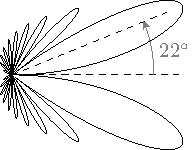
\includegraphics{emtAntennasAndRadiationTravellingWavePattern}
\caption*{الف: خطی اختتام کردہ مسلسل موج اینٹینا۔}
\end{subfigure}%
\begin{subfigure}{0.4\textwidth}
\centering
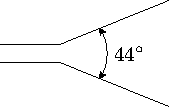
\includegraphics{emtAntennasAndRadiationTravellingWaveV}
\caption{ب: دو مسلسل موج اینٹینا کو \عددیء{44^{\circ}} پر رکھ کر بہتر سمتیت حاصل کی جاتی ہے۔}
\end{subfigure}%
\caption{}
\label{شکل_اینٹینا_مسلسل_موج_شعاع}
\end{figure}

شکل \حوالہ{شکل_اینٹینا_مسلسل_موج_شعاع}-الف میں \عددیء{n=20}اور \عددیء{d=\tfrac{\lambda}{4}} کی صورت میں حاصل \عددیء{4.75 \lambda} لمبائی کے اینٹینا کی شعاع دکھائی گئی ہے۔مرکزی شعاع \عددیء{\theta=22^{\circ}} پر پائی جاتی ہے۔جیسا شکل-ب میں دکھایا گیا ہے، دو عدد ایسے اینٹینا کو آپس میں \عددیء{44^{\circ}} کے میکانی زاویے پر رکھنے سے یک سمتی اینٹینا حاصل ہو گا جسے  دو تار کے ترسیلی تار سے طاقت مہیا کی جا سکتی ہے۔دونوں کے قریبی شعاع مل کر بہتر سمتیت دیتی ہے۔

زمین کے متوازی اینٹینا کا عمودی شعاع حاصل کرنے کی خاطر زمین میں اینٹینا کے عکس کو بھی مد نظر رکھا جائے گا۔

\حصہ{چھوٹا گھیرا اینٹینا} 
شکل \حوالہ{شکل_اینٹینا_دائرہ_چکور}-الف میں \عددیء{d} قطر کا \اصطلاح{گھیرا اینٹینا}\فرہنگ{گھیرا اینٹینا}\فرہنگ{اینٹینا!گھیرا}\حاشیہب{loop antenna}\فرہنگ{loop antenna} دکھایا گیا ہے جس میں \عددیء{I} برقی رو گزر رہی ہے۔ دائرے کا قطر طول موج سے بہت کم \عددیء{d \ll \lambda} ہے لہٰذا پورے گول دائرے پر یک قیمت اور ہم قدم برقی رو تصور کی جا سکتی ہے۔اس چھوٹے گول دائرے کو شکل-ب کا چکور تصور کرتے ہوئے، دور میدان حاصل کرتے ہیں۔چکور اور گول دائرے کے رقبے  برابر
\begin{align}
S=s^2=\frac{\pi d^2}{4} 
\end{align}
لئے جاتے ہیں۔ چکور کے چار اطراف کو چار جفت قطب تصور کرتے ہوئے دور میدان حاصل کیا جائے گا۔چکور کو کارتیسی محدد کے مرکز پر \عددیء{z=0} سطح پر رکھتے ہوئے \عددیء{x=0} سطح پر دور میدان حاصل کیا جائے گا۔سطح \عددیء{x=0} پر چکور کے اطراف الف اور پ برابر مگر الٹ سمت میں میدان پیدا کرتے ہیں لہٰذا ان کا مجموعہ صفر کے برابر ہے۔اطراف ب اور ت بطور مختصر جفت قطب کردار ادا کرتے ہیں جن کا نقش \عددیء{x=0} سطح پر غیر سمتی ہے لہٰذا انہیں دو غیر سمتی جفت قطب تصور کیا جا سکتا ہے۔ایسا ہی شکل-پ میں دکھایا گیا ہے جہاں سے دور میدان
\begin{align*}
E(\theta)=E_2 e^{-j\frac{\psi}{2}}-E_4e^{j\frac{\psi}{2}}
\end{align*}
لکھا جا سکتا ہے۔اس مساوات میں \عددیء{E_2=E_4} اور \عددیء{\psi=\beta s \sin \theta} ہیں۔یوں
\begin{align*}
E(\theta)=-j 2 E_2 \sin\left(\frac{\beta s}{2}\sin \theta \right) 
\end{align*}
لکھا جا سکتا ہے جسے \عددیء{s \ll \lambda} کی صورت میں
\begin{align}
E(\theta)=-j E_2 \beta s \sin \theta
\end{align}
لکھا جا سکتا ہے۔صفحہ \حوالہصفحہ{جدول_اینٹینا_مختصر_جفت_قطب} پر دیے گئے جدول \حوالہ{جدول_اینٹینا_مختصر_جفت_قطب} سے مختصر جفت قطب کے دور میدان \عددیء{E_{\theta}} کے حیطے کو \عددیء{E_2} کی جگہ پر کرتے ہوئے
\begin{align}
E(\theta)=\frac{60 \pi I l}{r \lambda} \beta s \sin \theta
\end{align}
حاصل ہوتا ہے۔شکل \حوالہ{شکل_اینٹینا_دائرہ_چکور}-پ میں جفت قطب کی لمبائی \عددیء{l=s} ہے جبکہ چکور کا رقبہ \عددیء{S=s^2} ہے لہٰذا
\begin{align}
E(\theta)=\frac{120 \pi^2 I}{r} \frac{S}{\lambda^2}\sin \theta
\end{align}
لکھا جا سکتا ہے۔مندرجہ بالا مساوات \عددیء{S} رقبے کے چھوٹے دائرے یا چکور کا دور میدان دیتی ہے۔چکور کا قطر جتنا کم ہو یہ مساوات اتنا ہی زیادہ درست میدان دیتا ہے۔حقیقت میں \عددیء{S} رقبے کے کسی بھی شکل کے چھوٹے بند دائرے کا دور میدان یہی مساوات دیتا ہے۔  

\begin{figure}
\centering
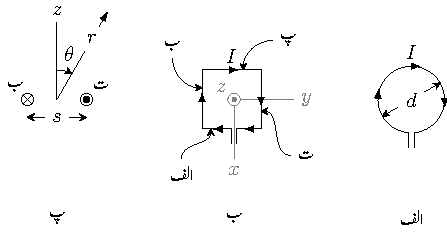
\includegraphics{emtAntennasAndRadiationLoopAntenna}
\caption{دائرہ اور چکور اینٹینا}
\label{شکل_اینٹینا_دائرہ_چکور}
\end{figure}

\حصہ{پیچ دار اینٹینا}
طول موج برابر محیط کا پیچ دار لچھا لمبائی جانب اخراجی اینٹینا کا کام کرتا ہے۔ایسے اینٹینا کی شعاع،  دائری قطبیت رکھتی ہے۔لچھے کی لمبائی اور  اینٹینا کی سمتیت راست تناسب کا تعلق رکھتے ہیں۔\اصطلاح{پیچ دار اینٹینا}\فرہنگ{پیچ دار اینٹینا}\فرہنگ{اینٹینا!پیچ دار}\حاشیہب{helical-beam antenna}\فرہنگ{helical-beam antenna} کا قطر \عددیء{D}،اس کا محیط \عددیء{C}، چکر کے مابین فاصلہ \عددیء{d}، چکر کی لمبائی \عددیء{l} اور پیچ دار زاویہ \عددیء{\alpha}، اس کے اہم ناپ ہیں۔ان تمام کو شکل \حوالہ{شکل_اینٹینا_پیچ_دار_الف} میں دکھایا گیا ہے۔ایسا لچھے جس  کا محیط \عددیء{C=\pi D} تقریباً  ایک طول موج \عددیء{(1\lambda)} لمبا ہو پر ایک مکمل موج پائی جائے گی۔یوں نصف چکر پر برقی موج کا مثبت حصہ اور بقایا پر موج کا منفی حصہ پایا جائے گا۔ لچھے کے ایک چکر کو شکل-پ میں دکھایا گیا ہے جہاں اس پر برقی رو اور برقی بار دکھائے گئے ہیں جو میدان \عددیء{\kvec{E}} پیدا کرتے ہیں۔جیسے جیسے برقی رو کی موج اینٹینا پر آگے حرکت کرتی ہے ویسے ویسے میدان \عددیء{\kvec{E}} گھومے گا جو اینٹینا کے محور پر \اصطلاح{دائری قطبیت}\فرہنگ{دائری قطبیت}\فرہنگ{قطبیت!دائری}\حاشیہب{circular polarization}\فرہنگ{circular polarization} کو جنم دے گی۔پیچ دار لچھا بطور مسلسل موج اینٹینا کردار ادا کرتا ہے اور اس کی خاصیت یہ ہے کہ اسے کسی مزاحمت سے اختتام پذیر کرنے کی ضرورت نہیں ہوتی۔اس پر برقی رو بالکل مسلسل موج اینٹینا کی مانند ہوتی ہے۔اینٹینا کے کھلے سر سے انعکاسی موج قابل نظرانداز ہونے کے ناطے، اس پر یکساں حیطے کے برقی رو کی موج خارجی جانب حرکت کرتی پائی جاتی ہے۔

\begin{figure}
\centering
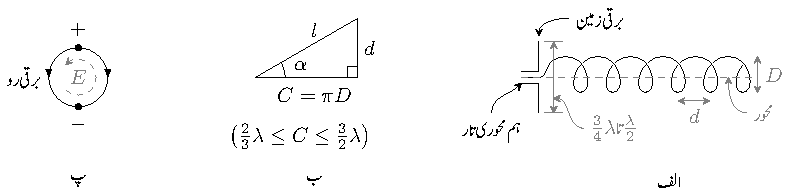
\includegraphics{emtAntennasAndRadiationHelicalDimensions}
\caption{پیچ دار اینٹینا۔}
\label{شکل_اینٹینا_پیچ_دار_الف}
\end{figure}

پیچ دار اینٹینا کو لمبائی جانب اخراجی قطار تصور کیا جا سکتا ہے جہاں ہر چکر کو انفرادی منبع فرض کیا جاتا ہے۔ضرب نقش کے اصول سے، انفرادی منبع کا نقش ضرب غیر سمتی ارکان کے  قطار کا نقش، 
\begin{align}\label{مساوات_اینٹینا_لمبی_پیچ_دار_اینٹینا}
E(\theta)=\cos \theta \frac{\sin (n\psi\!/\!2)}{\sin(\psi\!/\!2)}
\end{align}
اینٹینے  کا نقش دیتا ہے۔اس مساوات میں انفرادی چکر کے نقش کو \عددیء{\cos \theta} کے لگ بھگ تصور کیا گیا ہے۔مندرجہ بالا مساوات میں
\begin{align}\label{مساوات_اینٹینا_لمبی_پیچ_دار_اینٹینا_زاویائی_فرق}
\psi=\beta d \cos \theta- \frac{c \beta L}{v}
\end{align}
کے برابر ہے جہاں دو قریبی چکر کے مابین زاویائی فرق \عددیء{\tfrac{c \beta  L}{v}} ہو گا جو  ایک چکر گولائی \عددیء{L} پر \عددیء{v} رفتار سے حرکت کرتی موج کا زاویائی فرق ہے۔

مساوات \حوالہ{مساوات_اینٹینا_لمبی_پیچ_دار_اینٹینا} اور  مساوات \حوالہ{مساوات_اینٹینا_لمبی_مسلسل_موج_اینٹینا} کے موازنے سے معلوم ہوتا ہے کہ یہ قدر مختلف ہیں۔مساوات \حوالہ{مساوات_اینٹینا_لمبی_پیچ_دار_اینٹینا} میں \عددیء{\cos \theta} پایا جاتا ہے جس کی قیمت \عددیء{\theta=0} پر زیادہ سے زیادہ ہے جو اینٹینا کا محور یعنی شعاعی اخراج کی سمت  ہے۔اس کے برعکس مساوات \حوالہ{مساوات_اینٹینا_لمبی_مسلسل_موج_اینٹینا} میں \عددیء{\sin \theta} کا جزو ضربی پایا جاتا ہے جو اینٹینا کے محور پر صفر کے برابر ہے لہٰذا اس اینٹینا کی شعاع دو شاخی ہے اور اس کی سمتیت قدر کم ہے۔

چونکہ میدان دائری قطبی اور محور کے گرد یکساں ہے لہٰذا یہی مساوات \عددیء{E_{\theta}(\theta)} کے علاوہ \عددیء{E_{\phi}(\theta)} کا نقش بھی دیتی ہے۔

کسی بھی لمبائی جانب اخراجی قطار  میں تمام منبع کے میدان اینٹینا کے محور پر ہم قدم  ہوتے ہیں جو
\begin{align}
\psi=0, \mp 2\pi, \mp  4\pi, \cdots
\end{align}
کی صورت میں ممکن ہوتا ہے۔پیچ دار اینٹینا میں \عددیء{\psi=-2\pi} کے برابر ہے۔ارکان کے مابین \عددیء{\psi=-2\pi} زاویائی فرق کی بنیاد پر حاصل نقش اور اصل پیچ دار اینٹینا کے ناپے گئے نقش میں خاصہ فرق پایا جاتا ہے۔پیچ دار اینٹینا کی ناپی گئی سمتیت زیادہ ہے۔ہنسن اور ووڈیارڈ\حاشیہب{Hansen and Woodyard} یہ ثابت کر چکے ہیں کہ \عددیء{n} رکنی لمبائی جانب اخراجی قطار کی زیادہ سے زیادہ سمتیت اس صورت حاصل ہوتی ہے جب اس کے ارکان کے مابین \عددیء{\psi=-2\pi-\frac{\pi}{n}} زاویائی فرق پایا جاتا ہو۔مساوات \حوالہ{مساوات_اینٹینا_لمبی_پیچ_دار_اینٹینا} میں ارکان کے مابین زاویائی فرق \عددیء{\psi=-2\pi-\frac{\pi}{n}} پر کرنے سے حقیقی اینٹینا کے ناپے نقش  جیسا نقش حاصل ہوتا ہے۔اس سے ثابت ہوتا ہے کہ حقیقی اینٹینا پر دو قریبی چکر کے مابین یہی زاویائی فرق پایا جاتا ہے۔اس نتیجے کو تسلیم کرتے ہوئے مساوات \حوالہ{مساوات_اینٹینا_لمبی_پیچ_دار_اینٹینا_زاویائی_فرق} سے
\begin{align}
\psi=\beta d \cos \theta- \frac{c \beta L}{v}=-2\pi-\frac{\pi}{n}
\end{align}
لکھتے ہوئے  
\begin{align}
\frac{v}{c}=\frac{\frac{1}{\lambda}}{\frac{d}{\lambda}+\frac{2n+1}{2n}}
\end{align} 
حاصل ہوتا ہے۔یوں \عددی{C=\lambda}، \عددی{\alpha=12^{\circ}} اور \عددیء{n=20} کی صورت میں \عددیء{\tfrac{v}{c}=0.82} ہو گی۔
حقیقی پیچ دار اینٹینا پر موج کی رفتار یہی ناپی جاتی ہے۔ایسا معلوم ہوتا ہے کہ پیچ دار اینٹینا خود بخود موج کی رفتار کو اس قیمت پر رکھتی ہے جس پر اینٹینا کی سمتیت زیادہ سے زیادہ حاصل ہو۔تین سے زیادہ چکر پر مبنی پیچ دار اینٹینا یہ عمل \عددیء{(5^{\circ} < \alpha < 20^{\circ})} اور \عددیء{(\tfrac{3}{4}\lambda<C<\tfrac{3}{2}\lambda)} تک حاصل کرنے کی صلاحیت رکھتی ہے۔چکر کی تعداد بڑھا کر سمتیت بڑھائی جا سکتی ہے۔

پیچ دار اینٹینا کی سمتیت تقریباً
\begin{align}
D=15 \left(\frac{C}{\lambda}\right)^2 \frac{n d}{\lambda}
\end{align}
کے برابر ہے۔یوں \عددیء{C=\lambda} اور \عددیء{\alpha=12^{\circ}} کی صورت میں \عددیء{D=64} ہو گی۔

پیچ دار زاویہ \عددیء{\alpha=12^{\circ}} اور \عددیء{d=0.213\lambda} کی صورت میں طول موج میں تقریباً پانچ چکر پائیں جائیں گے لہٰذا \عددیء{20} چکر کا
 اینٹینا \عددیء{20 \times 0.213 \lambda=4.3\lambda} لمبائی کا ہو گا۔اتنی لمبائی کے عام لمبائی جانب اخراجی اینٹینا کی سمتیت چار گنا سے بھی قدر کم ہوتی ہے۔

پیچ دار اینٹینا کی سمتیت زیادہ ہونے کا مطلب ہے کہ اس کی اخراجی سطح حقیقی سطح سے بہت زیادہ ہوتی ہے۔مصنوعی سیاروں پر مبنی ذرائع ابلاغ میں پیچ دار اینٹینا کلیدی کردار ادا کرتی ہے۔ 

\حصہ{دو طرفہ کردار}
اینٹینا شعاع خارج کرتی ہے اور یا اسے وصول کرتی ہے۔اینٹینا کے تمام خاصیت دو طرفہ ہیں۔یوں اس کی سمتیت، اخراجی رقبہ، نقش اور اخراجی مزاحمت دونوں (اخراجی اور وصولی) صورتوں  میں برابر پائے جاتے ہیں۔البتہ اینٹینا پر برقی رو اخراجی اور وصولی صورت میں مختلف صورت رکھتی ہے۔

\begin{figure}
\centering
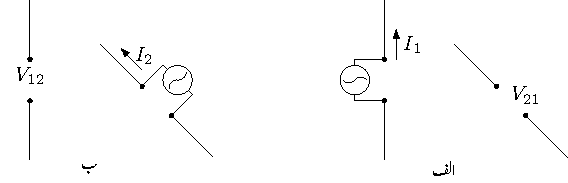
\includegraphics{emtAntennasAndRadiationReciprocity}
\caption{دو اینٹینا کے مابین باہمیت۔}
\label{شکل_اینٹینا_باہمیت}
\end{figure}
اینٹینا کی \اصطلاح{دو طرفہ خاصیت}\فرہنگ{دو طرفہ خاصیت}\فرہنگ{اینٹینا!دو طرفہ خاصیت}\حاشیہب{reciprocity}\فرہنگ{antenna!reciprocity} پر شکل \حوالہ{شکل_اینٹینا_باہمیت} کی مدد سے غور کرتے ہیں۔دونوں اینٹینا کے درمیان غیر متحرک، خطی اور غیر سمتی خطہ پایا جاتا ہے۔شکل-الف میں پہلے اینٹینا کو صفر رکاوٹ اور \عددیء{f} تعدد کے منبع سے طاقت مہیا کی جاتی ہے جس سے پہلے اینٹینا کے داخلی سروں پر \عددیء{I_1} برقی رو اور دوسرے اینٹینا کے کھلے برقی سروں پر برقی دباو \عددیء{V_{21}} پیدا ہوتی ہے۔اگر منبع طاقت کو دوسرے اینٹینا کے ساتھ جوڑا جائے تب دوسرے اینٹینا میں \عددیء{I_2} برقی رو اور پہلے اینٹینا کے کھلے برقی سروں پر \عددیء{V_{12}} برقی دباو پیدا ہو گا۔شکل-ب میں ایسا دکھایا گیا ہے۔چونکہ کسی بھی چار سروں والے برقی دور کا مساوی \عددیء{T} دور بنانا ممکن ہے لہٰذا ان اینٹینا کے چار برقی سروں کے مابین بھی ایسا کرنا ممکن ہو گا۔شکل \حوالہ{شکل_اینٹینا_مساوی_ٹی_دور} میں یہ مساوی دور دکھایا گیا ہے جہاں سے

\begin{figure}
\centering
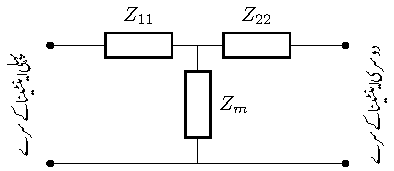
\includegraphics{emtAntennasAndRadiationEquivalentT}
\caption{مساوی $T$ دور۔}
\label{شکل_اینٹینا_مساوی_ٹی_دور}
\end{figure}

\begin{align*}
V_{21}&=I_1 Z_m\\
V_{12}&=I_2 Z_m
\end{align*}
یا
\begin{align}
\frac{V_{21}}{I_1}=\frac{V_{12}}{I_2}=Z_m
\end{align}
لکھا جا سکتا ہے۔دونوں اینٹینا کو  برابر برقی رو \عددیء{(I_1=I_2)} مہیا کرنے کی صورت میں
\begin{align}
V_{21}=V_{12}
\end{align}
ہو گا۔

\ابتدا{قانون}
اینٹینا کی دو طرفہ خاصیت کے تحت اگر کسی ایک اینٹینا کو برقی رو \عددیء{I} مہیا کی جائے جس سے کسی دوسرے اینٹینا میں برقی دباو \عددیء{V} پیدا ہو تب دوسرے اینٹینا کو برقی رو \عددیء{I} فراہم کرنے سے پہلے اینٹینا میں برقی دباو \عددیء{V} پیدا ہو گا۔
\انتہا{قانون}

دونوں اینٹینا کے مابین مشترکہ رکاوٹ \عددیء{Z_m} دونوں اطراف سے برابر ہے۔

\حصہء{نقش}
شکل \حوالہ{شکل_اینٹینا_نقش_ناپ} میں اینٹینا-الف شعاع خارج کر رہی ہے جبکہ اینٹینا-ب اس شعاع کو وصول کر رہی ہے۔اینٹینا-الف ساکن ہے جبکہ اینٹینا-ب اس کے گرد گول دائرے پر گھوم رہی ہے۔اینٹینا-ب پر پیدا برقی دباو، اینٹینا-الف کی نقش دے گی۔اب اگر دائرے پر گھومتی اینٹینا شعاع خارج کرے اور ساکن اینٹینا اس شعاع کو وصول کرے تو اینٹینا کے دو طرفہ خاصیت کے تحت وہی نقش دوبارہ حاصل ہو گا۔یوں کسی بھی اینٹینا کا اخراجی نقش اور وصولی نقش بالکل یکساں ہوتے ہیں۔اینٹینا کی دو طرفہ خاصیت اس کے نقش کے لئے بھی درست ثابت ہوتی ہے۔
\begin{figure}
\centering
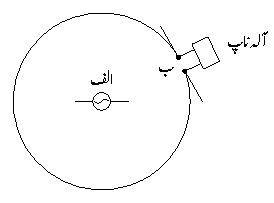
\includegraphics{emtAntennasAndRadiationPatternReciprocity}
\caption{نقش کی ناپ۔}
\label{شکل_اینٹینا_نقش_ناپ}
\end{figure}
\حصہء{سمتیت اور اخراجی رقبہ}
مساوات \حوالہ{مساوات_اینٹینا_سمتیت_کی_ایک_اور_مساوات}
\begin{align}
D=\frac{4\pi}{\iint \limits_{4\pi} P_n(\theta,\phi) \dif \Omega}
\end{align}
کے تحت سمتیت صرف اور صرف نقش پر منحصر ہے اور ہم دیکھ چکے ہیں کہ اینٹینا کا اخراجی نقش اور اس کا وصولی نقش بالکل یکساں ہوتے ہیں لہٰذا اس کی اخراجی سمتیت اور وصولی سمتیت بھی بالکل یکساں ہوں گے۔

اگر اخراجی سمتیت اور  وصولی سمتیت برابر ہوں تب مساوات \حوالہ{مساوات_اینٹینا_سمتیت_مختلف_تعرف}
\begin{align}
D=\frac{4\pi}{\lambda^2} S_{\text{اخراجی}}
\end{align}
کے تحت اخراجی رقبہ اور وصولی رقبہ بھی برابر ہوں گے۔اینٹینا کی دو طرفہ خاصیت سمتیت اور رقبے کے لئے بھی درست ثابت ہوتی ہے۔

\حصہء{اخراجی مزاحمت اور وصولی مزاحمت}
اخراجی اینٹینا کو صرف داخلی برقی سروں سے برقی رو مہیا کی جا سکتی ہے جبکہ وصولی اینٹینا کے تمام جسامت پر برقی دباو پیدا ہوتا ہے جس سے اینٹینا کی برقی رو عموماً اخراجی صورت سے مختلف ہو گی۔

اگر اینٹینا کو مختلف برقی رکاوٹوں کا مجموعہ تصور کیا جائے تب اگرچہ اس کے مختلف حصوں پر برقی رو مختلف ممکن ہے لیکن کسی بھی دو سروں کے مابین رکاوٹ تبدیل نہیں ہوتی۔یوں اینٹینا کے برقی سروں کے مابین برقی رکاوٹ کا دارومدار اینٹینا میں برقی رو کی صورت پر نہیں ہوتی۔اس کا اخراجی رکاوٹ اور وصولی رکاوٹ بالکل برابر ہوتے ہیں۔اینٹینا کی دو طرفہ خاصیت یہاں بھی قابل استعمال ہے۔

\حصہ{جھری اینٹینا}
وسیع موصل چادر میں \عددیء{\tfrac{\lambda}{2}} لمبائی کی جھری شکل \حوالہ{شکل_اینٹینا_جھری_اینٹینا}-الف میں دکھائی گئی ہے۔ اگر \عددیء{a a'} کو ترسیلی تار سے جوڑا جائے تو جھری کے گرد موصل چادر میں برقی رو کی وجہ سے شعاعی اخراج پیدا ہو گی۔جھری کو از خود موصل چادر فرض کرتے  اینٹینا تصور کیا جا سکتا ہے جس کی مدد سے  \اصطلاح{جھری اینٹینا}\فرہنگ{جھری اینٹینا}\فرہنگ{اینٹینا!جھری}\حاشیہب{slot antenna}\فرہنگ{slot antenna} کا میدان حاصل کیا جاتا ہے۔شکل-ب میں اسی \اصطلاح{تکملہ اینٹینا}\فرہنگ{تکملہ اینٹینا}\فرہنگ{اینٹینا!تکملہ}\حاشیہب{complementary antenna}\فرہنگ{complementary antenna} کو دکھایا گیا ہے۔ جھری اینٹینا کو \عددیء{a a'} پر طاقت چوڑائی کے اطراف کے مابین فراہم کی جاتی ہے جبکہ تکملہ اینٹینا کو لمبائی جانب کے اطراف کے مابین طاقت \عددیء{a a'} پر مہیا کی جاتی ہے۔یوں ان کے میدان آپس میں \عددیء{90^{\circ}} پر ہوں\فرہنگ{Booker's theory}\حاشیہب{Booker's theory} گے۔جھری اینٹینا کی اخراجی رکاوٹ \عددیء{Z_{g}} اور تکملہ اینٹینا کی اخراجی رکاوٹ \عددیء{Z_d} کا آپس میں تعلق
\begin{align}
Z_g = \frac{Z_0^2}{4 Z_{d}}
\end{align}
ہے جہاں \عددیء{Z_0=120\pi} خلاء کی قدرتی رکاوٹ ہے۔

\begin{figure}
\centering
\begin{subfigure}{0.4\textwidth}
\centering
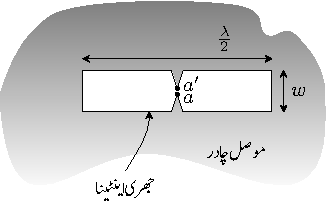
\includegraphics{emtAntennasAndRadiationSlotAntenna}
\caption*{الف: موصل چادر میں جھری بطور اینٹینا کام کرتی ہے۔}
\end{subfigure}%
%
\begin{subfigure}{0.4\textwidth}
\centering
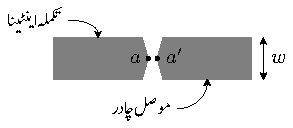
\includegraphics{emtAntennasAndRadiationSlotAntennaComplementary}
\caption*{ب: تکملہ اینٹینا کی مدد سے جھری اینٹینا پر غور کیا جاتا ہے۔}
\end{subfigure}%
\caption{جھری اینٹینا اور اس کا تکملہ اینٹینا۔}
\label{شکل_اینٹینا_جھری_اینٹینا}
\end{figure}

اس طرح جفت قطب کے خصوصیات جانتے ہوئے جھری کے خصوصیات دریافت کئے جا سکتے ہیں۔یوں اگر جھری کی چوڑائی \عددیء{c \ll \lambda} اور اس کی لمبائی \عددیء{\tfrac{\lambda}{2}} کر دی جائے تو تکملہ اینٹینا (صفحہ \حوالہصفحہ{صفحہ_اینٹینا_جفت_قطب_رکاوٹ}) کی اخراجی رکاوٹ \عددیء{Z_d=73+j 42.5}  جانتے ہوئے جھری اینٹینا کی اخراجی رکاوٹ
\begin{align}
Z_g=\frac{377^2}{4 \times (73+j42.5)}=363-j 211 \, \Omega
\end{align}
لکھی جا سکتی ہے۔

\حصہ{پیپا اینٹینا}
شکل \حوالہ{شکل_اینٹینا_پیپا_اینٹینا} میں \اصطلاح{پیپا اینٹینا}\فرہنگ{پیپا اینٹینا}\فرہنگ{اینٹینا!پیپا}\حاشیہب{horn antenna}\فرہنگ{horn antenna} دکھایا گیا ہے جسے بائیں جانب سے مستطیلی ترسیلی تار طاقت مہیا کر رہی ہے۔پیپا اینٹینا کو مستطیل ترسیلی تار کا کھلا منہ تصور کیا جا سکتا ہے۔مستطیلی ترسیلی تار کا منہ بڑھانے سے اینٹینا کی اخراجی سطح بڑھانا مقصد ہے جس سے سمتیت بڑھتی ہے۔اگرچہ پیپا کے منہ پر ہم قدم میدان ہی سے بہتر سمتیت حاصل ہو گی، حقیقت میں ایسا ہم قدم میدان حاصل کرنا ممکن نہیں ہوتا۔ یوں حقیقی اینٹینا میں پیپا کے منہ پر میدان میں فرق کو کسی مخصوص مقدار \عددیء{\delta} سے کم رکھا جاتا ہے۔شکل-ب کو دیکھ کر
  \begin{align*}
\cos \theta&=\frac{l}{l+\delta}\\
\sin \theta&=\frac{h}{2(l+\delta)}\\
\tan \theta&=\frac{h}{2l}
\end{align*}
لکھے جا سکتے ہیں۔کم \عددیء{\delta} کی صورت میں ان مساوات سے
\begin{align}
l&=\frac{h^2}{8 \delta}\\
\theta&=\tan^{-1} \frac{h}{2l}=\cos^{-1}\frac{l}{l+\delta}
\end{align}
لکھا جا سکتا ہے۔برقی میدان \عددیء{h} سمت میں اور مقناطیسی میدان \عددیء{w} سمت میں تصور کرتے ہوئے آگے پڑھیں۔برقی میدان \عددیء{E} کے سطح پر اس فرق کو \عددیء{\delta < \tfrac{\lambda}{5}} رکھا جاتا ہے جس سے پیپے کے منہ پر کل فرق \عددیء{\mp 36^{\circ}} تک محدود رہتا ہے جبکہ مقناطیسی میدان \عددیء{H} کے سطح  پر فرق \عددیء{\delta < \tfrac{3\lambda}{8}} تک محدود رکھا جاتا ہے۔مقناطیسی میدان کے سطح پیپے کے اطراف پر برقی میدان سطح کے متوازی ہونے کی وجہ سے صفر ہوتا ہے لہٰذا میدان میں زیادہ زاویائی فرق سے دور میدان زیادہ متاثر نہیں ہوتا۔

\begin{figure}
\centering
\begin{subfigure}{0.4\textwidth}
\centering
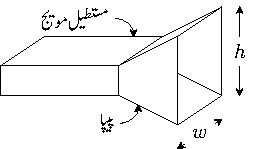
\includegraphics{emtAntennasAndRadiationHornAntenna}
\caption*{الف: پیپا اینٹینا۔}
\end{subfigure}%
%
\begin{subfigure}{0.4\textwidth}
\centering
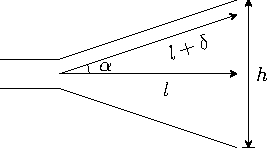
\includegraphics{emtAntennasAndRadiationHornAntennaSideView}
\caption*{ب: پیپا اینٹینا کے اہم ناپ۔}
\end{subfigure}%
\caption{پیپا اینٹینا اور اس کے اہم ناپ۔}
\label{شکل_اینٹینا_پیپا_اینٹینا}
\end{figure}
%===============
\ابتدا{مثال}
شکل میں \عددیء{h=10\lambda} ہے جبکہ ترسیلی تار میں \عددیء{\TE{10}} موج پائی جاتی ہے۔شکل میں \عددیء{}، \عددیء{w} اور نصف زاویے \عددیء{\theta} اور \عددیء{\phi} حاصل کریں۔

حل:
برقی میدان کی سطح پر \عددیء{\delta <\tfrac{\lambda}{5}} لیتے ہوئے 
\begin{align*}
l=\frac{h^2}{8 \delta}=\frac{100 \lambda^2}{8 \times \frac{\lambda}{5}}=62.5 \lambda
\end{align*}
حاصل ہوتا ہے جس سے \عددیء{E} سطح پر 
\begin{align*}
\theta=\tan^{-1}\frac{h}{2l}=\tan^{-1} \frac{10 \lambda}{2\times 62.5 \lambda}=4.6^{\circ}
\end{align*}
حاصل ہوتا ہے۔مقناطیسی میدان پر \عددیء{\delta <\tfrac{3\lambda}{8}} لیتے ہوئے 
\begin{align*}
\phi=\cos^{-1} \frac{62.5\lambda}{62.5\lambda+\frac{3}{8}\lambda}=6.26^{\circ}
\end{align*}
حاصل ہوتا ہے۔پیپے کی چوڑائی
\begin{align*}
w=2 l \tan \phi=2 \times 62.5 \times \lambda \times \tan 6.26^{\circ}=13.7 \lambda
\end{align*}
حاصل ہوتی ہے۔
\انتہا{مثال}
%================

\حصہ{فرائس ریڈار مساوات}
شکل \حوالہ{شکل_اینٹینا_ریڈار_الف} میں \عددیء{S_t} اخراجی رقبے کا ترسیل کنندہ  اور \عددیء{S_w} اخراجی رقبے کا وصول کنندہ اینٹینا آپس میں \عددیء{r} فاصلے پر دکھائے گئے ہیں۔اگر غیر سمتی ترسیل کنندہ  \عددیء{P_t} طاقت کی شعاع خارج کرے تب وصول کنندہ کے قریب اکائی رقبے پر 
\begin{align}
P=\frac{P_t}{4\pi r^2}
\end{align}
کثافت طاقت دستیاب ہو گی جس سے وصول کنندہ
\begin{align}
P_w'=P S_w
\end{align}
طاقت حاصل کر پائے گا۔ترسیلی سطح \عددیء{S_t} کے سمتی ترسیل کنندہ کی سمتیت \عددیء{D=\tfrac{4\pi S_t}{\lambda^2}} ہے لہٰذا اس کی شعاع سے وصول کنندہ
\begin{align}
P_w=D P_w'= \frac{4\pi S_t}{\lambda^2}\frac{P_t S_w}{4\pi r^2}
\end{align}
طاقت حاصل کر پائے گا۔اس مساوات سے
\begin{align}\label{مساوات_اینٹینا_ریڈار_الف}
\frac{P_w}{P_t}=\frac{S_t S_w}{\lambda^2 r^2}
\end{align}
لکھا جا سکتا ہے جہاں کسی بھی دو اینٹینا کے نظام میں مساوات کا دایاں ہاتھ بے بُعد مستقل ہے۔یہ مساوات \اصطلاح{فرائس ترسیلی مساوات}\فرہنگ{فرائس ترسیلی مساوات}\حاشیہب{Friis transmission equation}\فرہنگ{Friis transmission equation} کہلاتی ہے۔
\begin{figure}
\centering
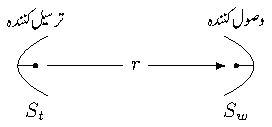
\includegraphics{emtAntennasAndRadiationFriisRadarEquation}
\caption{وصول کردہ طاقت کا انحصار ترسیلی اور وصولی اینٹینا کے اخراجی رقبوں پر ہے۔}
\label{شکل_اینٹینا_ریڈار_الف}
\end{figure}
آئیں اب شکل \حوالہ{شکل_اینٹینا_ریڈار_ب}-الف پر غور کریں  جہاں ترسیل کنندہ اینٹینا شعاع خارج کرتی ہے۔انعکاسی شعاع کو وصول کنندہ اینٹینا وصول کرتی ہے۔ریڈار میں عموماً ایک ہی اینٹینا دونوں کام سرانجام دیتی ہے۔شعاع کا انعکاس ہوا میں اڑتے جہاز سے ممکن ہے۔شکل \حوالہ{شکل_اینٹینا_ریڈار_ب}-ب میں عاکس کو دو اینٹینا کی صورت میں دکھایا گیا ہے جہاں ایک اینٹینا شعاع وصول کرتے ہوئے دوسرے اینٹینا سے واپس خارج کرتا ہے۔یوں مساوات \حوالہ{مساوات_اینٹینا_ریڈار_الف} کو دو مرتبہ استعمال کرتے ہوئے
\begin{align}
\frac{P_w}{P_t}=\frac{S_t S_w S^2_e}{\lambda^4 r^4}
\end{align}

لکھا جا سکتا ہے۔اگر ایک ہی اینٹینا بطور ترسیلی اور وصولی اینٹینا استعمال کیا جائے تب
\begin{align}\label{مساوات_اینٹینا_فرائس_الف}
\frac{P_w}{P_t}=\frac{S_w^2 S_e^2}{\lambda^4 r^4}
\end{align}
لکھا جا سکتا ہے جہاں عاکس کا اخراجی رقبہ \عددیء{S_e} ہے۔

اگر عاکس وسیع جسامت کا ہو اور اس سے انعکاسی موج عین ریڈار کی سمت میں ہو تب عاکس کا اخراجی رقبہ اس کے میکانی رقبے جتنا ہو گا۔عموماً عاکس غیر سمتی اخراج کرتا ہے جس کی وجہ سے اس کا اخراجی رقبہ، اس کے میکانی رقبے سے کم ہوتا ہے۔ایسی صورت میں عاکس کے وصولی رقبے کو \عددیء{\sigma} لکھتے ہوئے مساوات \حوالہ{مساوات_اینٹینا_ریڈار_الف} سے عاکس کی حاصل کردہ طاقت
\begin{align}
\frac{P}{P_t}=\frac{S_t \sigma}{\lambda^2 r^2}
\end{align}
لکھی جائے گی۔یہی طاقت غیر سمتی خارج کی جائے گی۔غیر سمتی اینٹینا کا اخراجی رقبہ \عددیء{S=\tfrac{\lambda^2}{4\pi}} ہوتا ہے۔یہی عاکس کی اخراجی رقبہ لیتے ہوئے مساوات \حوالہ{مساوات_اینٹینا_فرائس_الف} میں \عددیء{S_e^2=S \sigma} لکھتے ہوئے
\begin{align}
\frac{P_w}{P_t}=\frac{S_w^2 S \sigma}{\lambda^4 r^4}
\end{align}
یعنی
\begin{align}
\frac{P_w}{P_t}=\frac{S_w^2 \sigma}{4\pi \lambda^2 r^4}
\end{align}
حاصل ہوتا ہے جہاں \عددیء{\sigma} \اصطلاح{ریڈار رقبہ تراش}\فرہنگ{ریڈار!رقبہ تراش}\فرہنگ{رقبہ! ریڈار رقبہ تراش}\حاشیہب{radar cross section}\فرہنگ{radar cross section} کہلاتا ہے۔یہ \اصطلاح{ریڈار مساوات}\فرہنگ{ریڈار مساوات}\حاشیہب{radar equation}\فرہنگ{radar equation} کہلاتی ہے۔  

بڑی جسامت کی موصل کرہ، جس کا رداس \عددیء{a} ہو،  کی ریڈار رقبہ تراش اس کے میکانی رقبہ تراش \عددیء{\pi a^2} کے برابر ہوتی ہے۔غیر کامل عاکس کی صورت میں ریڈار رقبی تراش نسبتاً کم ہو گا، مثلاً ایک میٹر طول موج پر چاند کا ریڈار رقبہ تراش تقریباً \عددیء{\tfrac{1}{10}} گنا حاصل ہوتا ہے۔ 

\begin{figure}
\centering
\begin{subfigure}{0.4\textwidth}
\centering
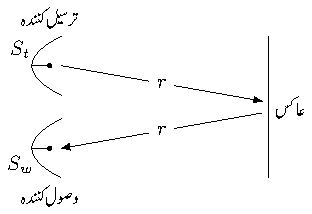
\includegraphics{emtAntennasAndRadiationFriisRadarEquationReflector}
\caption*{الف: عاکس سے انعکاسی موج کی وصولی۔}
\end{subfigure}%
%
\begin{subfigure}{0.4\textwidth}
\centering
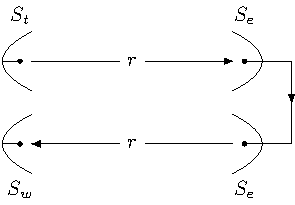
\includegraphics{emtAntennasAndRadiationFriisRadarEquationReflectorAsAntenna}
\caption*{ب: عاکس کو اینٹینا فرض کیا گیا ہے۔}
\end{subfigure}%
\caption{ریڈار اینٹینا شعاع خارج کر کے انعکاسی موج وصول کرتا ہے۔}
\label{شکل_اینٹینا_ریڈار_ب}
\end{figure}
%======================
\ابتدا{مثال}
ایک ٹی وی اسٹیشن موصل زمین پر کھڑے \عددیء{\SI{200}{\meter}} قد کے اینٹینا سے \عددیء{\SI{1}{\kilo \watt}} کی طاقت سے نشریات کرتی ہے۔افقی سطح پر اینٹینا غیر سمتی ہے جبکہ عمودی سمت میں اس کی نصف طاقت چوڑائی \عددیء{10^{\circ}} ہے۔طول موج \عددیء{\SI{1}{\meter}} ہونے کی صورت میں \عددیء{\SI{4}{\kilo\meter}} دور کتنی اونچائی پر اینٹینا بہترین وصولی کر پائے گا۔وصول کردہ طاقت کا بھی تخمینہ لگائیں۔وصولی اینٹینا مندرجہ ذیل فرض کرتے ہوئے حل کریں۔
\begin{itemize}
\item
عمودی قطبی اینٹینا جس کی سمتیت \عددیء{4} کے برابر ہے۔
\item
افقی قطبی اینٹینا جس کی سمتیت \عددیء{4} کے برابر ہے۔
\item
دائری قطبی \عددیء{6} چکر کا پیچ دار اینٹینا جس کا \عددیء{\alpha=12.5^{\circ}} اور چکر کے مابین فاصلہ \عددیء{0.22 \lambda} ہے۔
\end{itemize}

\begin{figure}
\centering
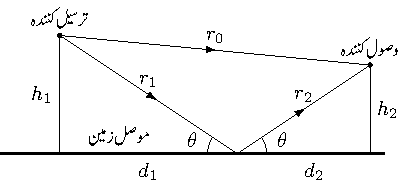
\includegraphics{emtAntennasAndRadiationTVreceptionExample}
\caption{سیدھی آمد موج اور انعکاسی موج کے اثرات۔}
\label{شکل_اینٹینا_سیدھی_آمد_انعکاسی_آمد}
\end{figure}


حل: شکل میں صورت حال دکھائی گئی ہے۔موصل زمین سے انعکاس پر زمین کے متوازی برقی میدان میں \عددیء{180^{\circ}} کی تبدیلی رو نما ہو گی۔یوں اگر وصولی اینٹینا زمین کے بالکل قریب ہو تب افقی قطبی میدان کی صورت میں یہ صفر طاقت وصول کر پائے گا جبکہ عمودی قطبیت کی صورت میں اسے سیدھی رسائی کے علاوہ زمین سے انعکاسی میدان بھی میسر ہو گا۔یوں کل میدان دگنا اور طاقت چار گنا ہو گا۔

شکل \حوالہ{شکل_اینٹینا_سیدھی_آمد_انعکاسی_آمد} کو دیکھتے ہوئے کہہ سکتے ہیں کہ کسی بھی \عددیء{h}  پر اگر
\begin{align}
r_1+r_2-r_0=n\lambda \quad \quad (n=0,1,2,\cdots)
\end{align}
ہو تب افقی قطبی میدان صفر پایا جائے گا جبکہ عمودی قطبی میدان دگنا ہو گا۔اسی طرح جب بھی
\begin{align}
r_1+r_2-r_0=n \frac{\lambda}{2} \quad \quad (n=1,3,5,\cdots)
\end{align}
ہو تب افقی قطبی میدان دگنا اور عمودی قطبی میدان صفر پایا جائے گا۔ان حقائق سے ظاہر ہے کہ زیادہ سے زیادہ افقی قطبی میدان کے دو قریبی نقطوں کے درمیانی نقطے پر زیادہ سے زیادہ عمودی قطبی میدان پایا جاتا ہے۔

بایاں دائری قطبی موج انعکاس کے بعد دایاں دائری قطبی ہوتا ہے۔اسی طرح دایاں دائری قطبی موج انعکاس کے بعد بایاں دائری قطبی ہوتا ہے۔یوں اگر ترسیلی اینٹینا دایاں دائری قطبی ہو تب دایاں دائری قطبی اینٹینا صرف سیدھے آمدی میدان کو وصول کر پائے گا جبکہ بایاں دائری قطبی اینٹینا صرف انعکاسی میدان کو وصول کر پائے گا۔یوں دونوں اقسام کے دائری قطبی اینٹینا اکائی میدان حاصل کریں گے۔ترسیلی اینٹینا بایاں قطبی ہونے کی صورت میں بایاں قطبی وصولی اینٹینا سیدھے آمد میدان کو وصول کرے گا جبکہ دایاں قطبی اینٹینا انعکاسی میدان کو وصول کرے گا۔

افقی اور عمودی قطبی اینٹینوں کی صورت میں وصولی اینٹینا کی اونچائی تبدیل کرنے سے میدان صفر تا دگنا حاصل کرنا ممکن ہے جبکہ دائری قطبی اینٹینا کی صورت میں وصول طاقت کا دارومدار اینٹینا کی اونچائی پر نہیں ہوتا۔دائری اینٹینا ہر صورت اکائی میدان حاصل کرتی ہے۔ 

چونکہ آمدی اور انعکاسی زاویے برابر ہوتے ہیں لہٰذا شکل میں آمدی تکون اور انعکاسی تکون یکساں ہیں۔یوں \عددیء{(r_1+r_2-r_0)} کی قیمت \عددیء{\tfrac{2h_1 h_2}{d}} لکھی جا سکتی ہے۔یوں عمودی قطب میدان کی زیادہ سے زیادہ قیمت
\begin{align*}
h_2=\frac{d \lambda}{2 h_1}=\frac{4\times 10^3 \times 1}{2 \times 200}=\SI{10}{\meter}
\end{align*}
کی صورت میں حاصل ہو گی جس سے افقی قطبی میدان کی زیادہ سے زیادہ قیمت کی اونچائی \عددیء{5}، \عددیء{15}، \عددیء{25}، \عددیء{\cdots} میٹر لکھی جا سکتی ہے۔

فرائس کی مساوات سے، ایک راہ سے موصول طاقت
\begin{align*}
P_w=\frac{P_t A_t A_w}{r^2 \lambda^2}=\frac{10^3\times0.32\times0.91}{16\times 10^6 \times 1}=\SI{18}{\micro \watt}
\end{align*}
حاصل ہوتی ہے جہاں ترسیلی اینٹینا کی سمتیت
\begin{align*}
D=\frac{4\pi}{\theta_{HP} \phi_{HP}}=\frac{4\pi}{\frac{360 \times \pi}{180} \times \frac{10 \times \pi}{180}}= 11.459
\end{align*}
لیتے ہوئے اس کا اخراجی رقبہ 
\begin{align*}
A_t=\frac{\lambda^2}{4\pi} D=\SI{0.91}{\meter \squared}
\end{align*}
اور وصولی اینٹینا کا وصولی رقبہ
\begin{align*}
A_w=\frac{\lambda^2}{4\pi}D=\frac{1^2 \times 4}{4\pi}=\SI{0.32}{\meter\squared}
\end{align*}
لئے گئے ہیں۔سیدھی آمد اور انعکاسی آمد میدان مل کر زیادہ سے زیادہ طاقت \عددیء{4} گنا کر دیتی ہیں۔یوں افقی قطبی اور عمودی قطبی اینٹینا کی صورت میں زیادہ سے زیادہ وصول کردہ طاقت \عددیء{\SI{72}{\micro\watt}} ہو گا جبکہ دونوں صورتوں میں کم سے کم حاصل کردہ طاقت صفر ہو گا۔ 
 

دائری قطبی صورت میں وصولی اینٹینا کی سمتیت
\begin{align*}
D=15 \left(\frac{C}{\lambda}\right)^2\frac{n d}{\lambda}=15 \left(\frac{\frac{0.22}{\tan 12.5^{\circ}}}{1} \right)^2\times \frac{6 \times 0.22}{1}=19.5
\end{align*}
اور وصولی رقبہ
\begin{align*}
A_w=\frac{\lambda^2 D}{4\pi}=\SI{1.55}{\meter\squared}
\end{align*}
ہیں لہٰذا ہر اونچائی پر وصول کردہ طاقت
\begin{align*}
P_w=\frac{1.55}{0.32} \times 18=\SI{87}{\micro \watt}
\end{align*}
ہو گا۔

وصول کردہ طاقت کا تخمینہ لگاتے ہوئے ہم نے اینٹینوں کے درمیان فاصلے کو چار کلو میٹر ہی تصور کیا اگرچہ حقیقی فاصلے قدر مختلف ہیں۔چار کلو میٹر کے فاصلے پر چند میٹر کم یا زیادہ سے حاصل جواب میں کوئی خاص تبدیلی پیدا نہیں ہوتی۔
\انتہا{مثال}
%===========

\حصہ{ریڈیائی دوربین، اینٹینا کی حرارت اور تحلیلی کارکردگی}
کسی بھی برقی مزاحمت \عددیء{R} میں حرارت \عددیء{T} کی وجہ سے آزاد بار حرکت کرتے ہیں جس سے مزاحمت میں \اصطلاح{حراری شور}\فرہنگ{شور!حراری}\فرہنگ{شور!برقی}\حاشیہب{thermal noise}\فرہنگ{thermal noise} پیدا ہوتا ہے۔ایسی مزاحمت کے برقی سروں پر \عددیء{B} تعددی پٹی پر 
\begin{align}\label{مساوات_اینٹینا_طاقت_شور_الف}
W=k B T
\end{align}
\اصطلاح{طاقت شور}\فرہنگ{شور!طاقت}\فرہنگ{طاقت!حراری شور}\حاشیہب{noise power}\فرہنگ{noise!power} پایا جاتا ہے۔اکائی تعددی پٹی پر یوں
\begin{align}
w=kT
\end{align}
طاقت شور پایا جائے گا جہاں
\begin{description}
\جزو{$w$} اکائی تعددی پٹی پر شور کی طاقت، \عددیء{\si{\watt \per \hertz}} 
\جزو{$k$} بولٹزمن کا مستقل، \عددیء{\SI{1.38e-23}{\joule \per \kelvin}}
\جزو{$B$} تعددی پٹی، \عددیء{\si{\hertz}}
\جزو{$T$} مزاحمت کی حتمی حرارت، \عددیء{\si{\kelvin}}
\end{description}
ہیں۔ \عددیء{T} کو \اصطلاح{حرارت شور}\فرہنگ{حرارت!شور}\فرہنگ{شور!حرارت}\حاشیہب{noise temperature}\فرہنگ{noise!temperature} کہا جاتا ہے۔برابر تعددی پٹی پر برابر طاقت شور پایا جاتا ہے۔

اگر برقی مزاحمت \عددیء{R} کے برابر اخراجی مزاحمت \عددیء{(R_{\text{اخراجی}}=R)} کے اینٹینا کے برقی سروں پر طاقت شور ناپی جائے تو یہ مزاحمت پر ناپی گئی طاقت شور سے مختلف ہو گی۔اینٹینا کے سروں پر طاقت شور، خلاء کے اس خطے کی حرارت \عددیء{T} سے پیدا شور ہو گا جہاں سے اینٹینا طاقت وصول کر رہا ہو۔اس طاقت شور کا اینٹینا کی حرارت سے کوئی تعلق نہیں۔یوں اینٹینا کو بطور \اصطلاح{بعید پیما حرارت}\فرہنگ{بعید پیما حرارت}\فرہنگ{حرارت!بعید پیما}\حاشیہب{remote temperature sensor}\فرہنگ{temperature sensor!remote} استعمال کیا جا سکتا ہے۔

ایک سنٹی میٹر طول موج کے ریڈیائی دوربین کی مرکز نگاہ  آسمان کے ایسے خطوں پر رکھی جا سکتی ہے جہاں حتمی حرارت \عددیء{\SI{0}{\kelvin}} کے قریب قریب ہوتی ہے۔ایسی صورت میں طاقت شور آسمان کی حرارت سے پیدا ہو گا نا کہ اینٹینا کے حرارت سے جو \عددیء{\SI{300}{\kelvin}} کے لگ بھگ  ہو گی۔ریڈیائی دوربین کی طاقت شور فی تعدد
\begin{align}
w=k T_A  \quad \quad (\si{\watt \per \hertz})
\end{align}
لکھی جاتی ہے جہاں \عددیء{T_A} اینٹینا کی حراری شور ہے جسے عموماً \اصطلاح{حرارت اینٹینا}\فرہنگ{حرارت!اینٹینا}\فرہنگ{اینٹینا!حرارت}\حاشیہب{antenna temperature}\فرہنگ{antenna!temperature} یا اخراجی مزاحمت کی حرارت کہا جاتا ہے۔حرارت اینٹینا وہ خطہ کرتی ہے جس پر اینٹینا کے نقش کی نظر ہو۔یوں اینٹینا کی مدد سے دور آسمان  کے خطوں کی حرارت ناپنا ممکن ہے۔ہم نے اس پورے بحث میں یہ فرض کر رکھا ہے کہ اینٹینا بے ضیاع ہے اور یہ آسمان کی طرف نظر رکھے ہوئے ہے۔یوں انعکاسی شعاع اور ثانوی شعاع کو رد کیا گیا ہے۔

ریڈیائی دوربین کو استعمال کرتے ہوئے  کثافت طاقت شور فی تعدد
\begin{align}
p=\frac{w}{S_e}=\frac{k T_A}{S_e} \quad \quad (\si{\watt \per \meter \squared \per\hertz})
\end{align} 
کا استعمال زیادہ سودمند ثابت ہوتا ہے جسے پوئنٹنگ سمتیہ فی تعدد تصور کیا جا سکتا ہے۔ 

اگر ہمیں منبع شور کی زاویائی وسعت \عددیء{\Omega_M} معلوم ہو اور یہ \عددیء{\Omega_A} کی نسبت سے کم ہو تب منبع کی حرارت
\begin{align}\label{مساوات_اینٹینا_ریڈیائی_حرارت}
\frac{T_A}{T_M}=\frac{\Omega_M}{\Omega_A}
\end{align}
سے حاصل کی جا سکتی ہے۔یاد رہے کہ \عددیء{T_A} کا اینٹینا کی حرارت سے کوئی تعلق نہیں۔

%===========
\ابتدا{مثال}
مریخ\فرہنگ{مریخ}\حاشیہب{Mars}\فرہنگ{Mars} پر مرکز نگاہ رکھتے ہوئے \عددیء{\SI{15}{\meter}} لمبی ریڈیائی دوربین کی اینٹینا حرارت \عددیء{\SI{31.5}{\milli\meter}} طول موج پر \عددیء{\SI{0.24}{\kelvin}} ناپی جاتی ہے۔اینٹینا پر مریخ \عددیء{0.005^{\circ}} زاویہ بناتا ہے اور اینٹینا کا نصف طاقت زاویہ \عددیء{0.116^{\circ}} ہے۔مریخ کی حرارت دریافت کریں۔

حل:مساوات \حوالہ{مساوات_اینٹینا_ریڈیائی_حرارت} سے مریخ کی حرارت
\begin{align*}
T_M=\frac{\Omega_A}{\Omega_M}T_A \approx \frac{0.116^2}{\pi (0.005^2\!/\!4)} 0.24=\SI{164}{\kelvin}
\end{align*}
حاصل ہوتی ہے۔
\انتہا{مثال}
%===========

\حصہ{حرارت نظام اور  حرارت بعید}
حرارت اینٹینا سے اس خطے کی حرارت حاصل کی جا سکتی ہے جس پر اینٹینا کا مرکز نگاہ ہو۔یوں اینٹینا کو بعید پیما حرارت استعمال کیا جا سکتا ہے۔ایک سنٹی میٹر طول موج کے ریڈیائی دوربین کی نگاہ، ستاروں سے خالی آسمان کے خطے پر رکھتے ہوئے انتہائی کم اینٹینا حرارت  حاصل کی جا سکتی ہے۔آسمان کو دیکھتے ہوئے کم تر حرارت \عددیء{\SI{3}{\kelvin}} حاصل ہوتی جو کائنات کی \اصطلاح{ابتدائی دھماکے}\فرہنگ{ابتدائی دھماکا}\فرہنگ{دھماکا!ابتدائی}\حاشیہب{big bang}\فرہنگ{big bang} کی \اصطلاح{بقیہ حرارت}\فرہنگ{بقیہ حرارت}\فرہنگ{حرارت!بقیہ}\حاشیہب{residual temperature}\فرہنگ{residual temperature}\فرہنگ{temperature!residual} ہے۔اگر اینٹینا کے سامنے ستارہ موجود ہو تب بقیہ حرارت سے زیادہ حرارت ناپی جائے گی۔ایک میٹر طول موج پر ہماری کہکشاں کی حرارت کئی ہزار کیلون ناپی جاتی ہے۔ہم \اصطلاح{حراری}\فرہنگ{حراری}\حاشیہب{thermal} شور کی حرارت ناپنے کی بات کر رہے ہیں۔یہ کامل اخراجی-وصولی خاصیت کے جسم کی حرارت ہے۔ایسے جسم کو  \اصطلاح{سیاہ جسم}\فرہنگ{سیاہ جسم}\حاشیہب{blackbody}\فرہنگ{blackbody} کہا جاتا ہے۔یوں اگر اینٹینا کی پوری وصولی نقش کے خطے میں گرم کوئلے یا سیاہ دھات کا کرہ پایا جائے، تو اینٹینا سے کرہ کی ناپی گئی حرارت وہی ہو گی جو \اصطلاح{تھرمامیٹر}\فرہنگ{تھرمامیٹر}\حاشیہب{thermometer}\فرہنگ{thermometer} سے ناپی جائے گی۔اس کے  برعکس ترسیلی اینٹینا کی ناپی گئی اینٹینا حرارت غیر یقینی طور پر زیادہ حاصل ہوتی ہے۔   

مثال کے طور پر  اگر قریب ریڈیو اسٹیشن کی نشریات، \عددیء{\SI{10}{\meter\squared}} وصولی رقبے اور \عددیء{\SI{10}{\kilo\hertz}} تعددی پٹی کے وصولی اینٹینا کے قریب \عددیء{\SI{10}{\micro\volt\per\meter}} کا میدان پیدا کرے تو وصولی اینٹینا کی کل وصول کردہ طاقت
\begin{align*}
W=\frac{E^2}{Z_0} S_e=\frac{10^{-10}}{377} \times 10=\SI{2.65}{\pico \watt}
\end{align*}
ہو گی جسے مساوات \حوالہ{مساوات_اینٹینا_طاقت_شور_الف} میں پر کرتے ہوئے
\begin{align*}
T=\frac{W}{k B}=\frac{2.65\times 10^{-12}}{1.38\times 10^{-23}\times 10^4}=\SI{1.9e7}{\kelvin}
\end{align*}
حاصل ہوتی ہے۔اس مثال میں آپ نے دیکھا کہ صرف \عددیء{\SI{10}{\micro\volt\per\meter}} کا میدان  \عددیء{\SI{1.9e7}{\kelvin}} کی اینٹینا حرارت پیدا کر سکتا ہے۔یہ اتنی بڑی مقدار ہے کہ اس کی موجودگی میں بقایا نظام کی حرارت، جسے \اصطلاح{حرارت نظام}\فرہنگ{حرارت!نظام}\فرہنگ{نظام!حرارت}\حاشیہب{system temperature}\فرہنگ{temperature!system} پکارا جاتا ہے، کو نظر انداز کیا جا سکتا ہے۔البتہ، ریڈیائی دوربین اتنی کم طاقت کے اشارات پر کام کرتے ہیں کہ ان میں حرارت نظام انتہائی اہم ہوتا ہے۔اس کا اندازہ آپ یوں کر سکتے ہیں کہ ریڈیائی دوربین کے استعمال میں کثافت طاقت فی ہرٹز کی اکائی \اصطلاح{جانسکی}\فرہنگ{جانسکی}\حاشیہب{Jansky}\فرہنگ{Jansky} ہے جہاں \عددیء{\SI{1}{Ja}=\SI{e-26}{\watt\per\meter\squared\per\hertz}} کے برابر ہے۔

\newpage
\حصہء{سوالات}

\ابتدا{سوال}
غیر سمتی اینٹینا \عددی{E=\frac{25 I}{r}} میدان پیدا کرتی ہے جہاں اینٹینا کا داخلی موثر برقی رو \عددی{I} اور اینٹینا سے فاصلہ \عددی{r} ہے۔اس اینٹینا کی اخراجی مزاحمت حاصل کریں۔

جواب:\عددی{\SI{20.8}{\ohm}}
\انتہا{سوال}
%=======================
\ابتدا{سوال}
اینٹینا کی شعاع \عددی{0<\theta<30^{\circ}}، \عددی{0<\phi<2\pi} خطے میں یکساں میدان پیدا کرتی ہے جبکہ \عددی{30^{\circ}<\theta<180^{\circ}} خطے میں میدان صفر کے برابر ہے۔ الف) اینٹینا کا اخراجی ٹھوس زاویہ \عددی{\Omega_A} حاصل کریں۔ ب) شعاع کی سمتیت \عددی{D} دریافت کریں۔

جوابات: \عددی{\SI{0.842}{\steradian}}، \عددی{14.9}
\انتہا{سوال}
%=====================
\ابتدا{سوال}

اینٹینا کی شعاع \عددی{0<\theta<60^{\circ}}، \عددی{0<\phi<2\pi} خطے میں یکساں میدان پیدا کرتی ہے جبکہ \عددی{60^{\circ}<\theta<180^{\circ}} خطے میں میدان صفر کے برابر ہے۔ الف) اینٹینا کا اخراجی ٹھوس زاویہ \عددی{\Omega_A} حاصل کریں۔ ب) شعاع کی سمتیت \عددی{D} دریافت کریں۔ پ) اینٹینا کا اخراجی رقبہ \عددی{A_e} حاصل کریں۔ ت) اینٹینا کا داخلی موثر برقی رو \عددی{\SI{12}{\ampere}} ہونے کی صورت میں اینٹینا سے \عددی{\SI{164}{\meter}} کے فاصلے پر موثر برقی 
میدان \عددی{\SI{7}{\volt\per\meter}} ہے۔ اینٹینا کا اخراجی مزاحمت \عددی{R_{\text{اخراجی}}} دریافت کریں۔



جوابات: \عددی{\SI{3.142}{\steradian}}، \عددی{4}، \عددی{0.318\lambda^2}، \عددی{\SI{76.3}{\ohm}}
\انتہا{سوال}
%===================
\ابتدا{سوال}
اینٹینا کی شعاع \عددی{45^{\circ}<\theta<60^{\circ}}، \عددی{0^{\circ}<\phi<120^{\circ}} خطے میں یکساں ہے۔بقایا خطے میں میدان صفر کے برابر ہے۔اینٹینا سے \عددی{\SI{1000}{\meter}} کے فاصلے پر اس خطے میں \عددی{\SI{2}{\volt\per\meter}} برقی میدان حاصل کرنے کی خاطر \عددی{\SI{4}{\ampere}} موثر داخلی برقی رو درکار ہے۔ اینٹینا کی اخراجی مزاحمت \عددی{R_{\text{اخراجی}}} دریافت کریں۔

جواب:\عددی{\SI{288}{\ohm}}
\انتہا{سوال}
%=================
\ابتدا{سوال}
اینٹینا کی مرکزی شعاع  \عددی{0^{\circ}<\theta<45^{\circ}} خطے میں یکساں پائی جاتی ہے جبکہ اس کی ثانوی شعاع \عددی{120^{\circ}<\theta<180^{\circ}} خطے میں یکساں پائی جاتی ہے۔میدان \عددی{\phi} کے ساتھ تبدیل نہیں ہوتا۔مرکزی شعاع میں میدان ثانوی شعاع کے میدان کے چار گنا ہے۔ الف) اینٹینا کی سمتیت \عددی{D} دریافت کریں۔ب) مرکزی شعاع میں اینٹینا سے \عددی{\SI{350}{\meter}} فاصلے پر \عددی{E_{\text{موثر}}=\SI{6}{\volt\per\meter}} برقی میدان کے حصول کے لئے اینٹینا کو \عددی{\SI{6}{\ampere}}  موثر داخلی برقی رو مہیا کیا جاتی ہے۔اینٹینا کی اخراجی مزاحمت \عددی{R_{\text{اخراجی}}} دریافت کریں۔

جوابات:\عددی{D=6.17}، \عددی{\SI{662}{\ohm}}
\انتہا{سوال}
%======================
\ابتدا{سوال}
دو عدد غیر سمتی، ہم قدم منبع کے درمیان فاصل \عددی{2\lambda} ہے۔ الف) نقش کے صفر حاصل کریں۔ ب) نقش کی چوٹیاں حاصل کریں۔

جوابات:الف) \عددی{\mp 41.4^{\circ}}، \عددی{\mp 75.5^{\circ}}، \عددی{\mp 104.5^{\circ}}، \عددی{\mp 138.6^{\circ}}؛ ب) \عددی{0^{\circ}}، \عددی{\mp 60^{\circ}}، \عددی{\mp 90^{\circ}}، \عددی{\mp 120^{\circ}}، \عددی{180^{\circ}}
\انتہا{سوال}
%=====================
%======================
\ابتدا{سوال}
دو عدد غیر سمتی، منبع کے درمیان فاصل \عددی{\tfrac{3\lambda}{2}} ہے جبکہ ان میں زاویائی فرق \عددی{180^{\circ}} ہے۔ الف) نقش کے صفر حاصل کریں۔ ب) نقش کی چوٹیاں حاصل کریں۔

جوابات:الف) \عددی{\mp 90^{\circ}}، \عددی{\mp 48.2^{\circ}}، \عددی{\mp 131.8^{\circ}}؛ ب) \عددی{0^{\circ}}، \عددی{\mp 70.5^{\circ}}، \عددی{\mp 109.5^{\circ}}
\انتہا{سوال}
%=====================
\ابتدا{سوال}
چار رکنی قطار میں غیر سمتی،  یکساں طاقت کے منبع پائے جاتے ہیں۔قطار میں ہر دو قریبی منبع میں \عددیء{\delta} زاویائی فرق پایا جاتا ہے۔منبع کے درمیان فاصلہ نصف طول موج سے کم \عددی{d<\tfrac{\lambda}{2}} ہے۔زیادہ سے زیادہ میدان \عددی{\theta=45^{\circ}} پر  اور نقش کا صفر \عددی{\theta=90^{\circ}} پر حاصل کرنے کے لئے درکار \عددی{\delta} اور \عددی{d} حاصل کریں۔ 

جوابات:\عددی{\delta=-90^{\circ}}، \عددی{d=0.354\lambda}
\انتہا{سوال}
%==========================
\ابتدا{سوال}
گھریلو ریڈیو سے \عددی{\SI{585}{\kilo\hertz}} تعدد کی نشریات سنی جا رہی ہے۔ الف) ریڈیو اینٹینا کو غیر سمتی تصور کرتے ہوئے اس کا اخراجی رقبہ دریافت کریں۔ ب) گھر سے ریڈیو اسٹیشن کا فاصلہ \عددی{\SI{10}{\kilo\meter}} جبکہ اسٹیشن کی اخراجی طاقت \عددی{\SI{5}{\kilo\watt}} کی صورت میں ریڈیو کتنی طاقت وصول کر پاتا ہے۔اسٹیشن کی اخراج غیر سمتی تصور کریں۔ پ) ریڈیو کی داخلی مزاحمت \عددی{\SI{300}{\ohm}} ہے۔ریڈیو کو صرف \عددی{\SI{1}{\micro\volt}} موثر داخلی اشارہ درکار ہے۔درکار داخلی طاقت کی قیمت حاصل کریں۔  

جوابات:\عددی{\SI{20928}{\meter\squared}}، \عددی{\SI{83.3}{\milli\watt}}، \عددی{\SI{3.33}{\femto\watt}}
\انتہا{سوال}
%=======================
\ابتدا{سوال}
\عددیء{1.5 \lambda} لمبے خطی اینٹینا کا اخراجی مزاحمت حاصل کریں۔ایسا کرنے کی خاطر آپ کو صفحہ \حوالہصفحہ{جدول_اینٹینا_عددی_اخراجی_مزاحمت} پر دیے جدول \حوالہ{جدول_اینٹینا_عددی_اخراجی_مزاحمت} کے طرز کا جدول حاصل کرنا ہو گا۔

جواب: \عددیء{\SI{100}{\ohm}}
\انتہا{سوال}
%==================
\ابتدا{سوال}
یکساں غیر سمتی منبع پر مبنی قطار میں ارکان کے درمیان \عددیء{d=\tfrac{\lambda}{4}} ہے۔مرکزی شعاع \عددیء{\theta=30^{\circ}} پر حاصل کرنے کی خاطر ارکان کے مابین زاویائی فرق \عددیء{\delta} حاصل کریں۔ 

جواب: \عددیء{\SI{1.36}{\radian}}
\انتہا{سوال}
%===============
\ابتدا{سوال}
تداخل پیما میں  جفت قطب کے مابین فاصلہ \عددیء{10\lambda} ہونے کی صورت میں پہلے صفر چوڑائی حاصل کریں۔

جواب: \عددیء{5.7^{\circ}}
\انتہا{سوال}
%================
\ابتدا{سوال}
خلاء میں دو مصنوعی سیاروں  کے درمیان \عددی{\SI{2e8}{\meter}} کا فاصلہ ہے۔یہ آپس میں \عددی{\SI{2.5}{\giga\hertz}} تعدد پر اشارات کا تبادلہ  کرتے ہیں۔دونوں سیارے \عددی{D=1500} سمتیت  کے اینٹینا استعمال کرتے ہیں۔اطلاعات صحیح موصول ہونے کے لئے ضروری ہے کہ حاصل کردہ اشارے کی طاقت  برقی شور سے قدر زیادہ ہو۔ یوں ضروری ہے کہ حاصل کردہ برقی اشارے کی طاقت کم از کم \عددی{\SI{1}{\pico\watt}} ہو۔ اخراجی اینٹینا کی درکار طاقت حاصل کریں۔

جواب:\عددی{\SI{195}{\watt}}
\انتہا{سوال}
%==============
